\documentclass[12pt, oneside]{report}

\usepackage[left=2.5cm, top=2.5cm, bottom=2.5cm, right=2.5cm]{geometry}

\usepackage[backend=bibtex,style=numeric,sorting=none]{biblatex}
\bibliography{bibliography}

\usepackage[utf8]{inputenc}
\usepackage[T1]{polski}
\usepackage[polish,english]{babel}
\selectlanguage{polish}
\usepackage{amsmath}
\usepackage{svg}
\usepackage{pdfpages}
\usepackage{float}
\usepackage{subcaption}

\begin{document}
\thispagestyle{empty}
\begin{titlepage}
    \begin{center}

           \Large
	\textbf{Uniwersytet Jagielloński w Krakowie}\vspace{0.2cm}\\ Wydział Fizyki, Astronomii i Informatyki Stosowanej
               \vspace*{1cm}

         \vspace{3cm}
         \Large
          \textbf{Jakub Wida}\\\vspace{0.5cm}
         \normalsize Nr albumu: 1113470\\
             \vspace{2cm}
        \Huge
        \textbf{Random Sequential Adsorption of particles built of disks using GPU}

        \vspace{1.5cm}
        \normalsize
        Praca magisterska\\
        na kierunku Informatyka Stosowana\\ \vspace{0.15cm}

        \vfill
        \vspace{2cm}
       \begin{minipage}{1\textwidth}
\begin{flushright}
Praca wykonana pod kierunkiem\\
dr. hab. Michała Cieśli\\
z Zakładu Fizyki Statystycznej
\end{flushright}
\end{minipage}

        \vspace{2cm}
        \begin{center}
      Kraków 2019
        \end{center}
    \end{center}
\end{titlepage}

\newpage
 \thispagestyle{empty}
\vspace{2.5cm}
\begin{flushleft}
\large \textbf{Oświadczenie autora pracy}\vspace{0.6cm}\\
\end{flushleft}

\noindent Świadom odpowiedzialności prawnej oświadczam, że niniejsza praca dyplomowa została napisana przeze mnie samodzielnie i nie zawiera treści uzyskanych w sposób niezgodny z obowiązującymi przepisami.\\

\noindent Oświadczam również, że przedstawiona praca nie była wcześniej przedmiotem procedur związanych z uzyskaniem tytułu zawodowego w wyższej uczelni.
\vspace{2cm}
\begin{center}
\begin{tabular}{lr}
................................~~~~~~~~~~~~~~~~~~~~~~~~~~~~~~~~~~~~~~&
.......................................... \\
{~~~~Kraków, dnia} & {Podpis autora pracy~~~~}
\end{tabular}
\end{center}
\vspace{5cm}
\begin{flushleft}
\large \textbf{Oświadczenie kierującego pracą}
\end{flushleft}

\noindent Potwierdzam, że niniejsza praca została przygotowana pod moim kierunkiem i~kwalifikuje się do przedstawienia jej w postępowaniu o nadanie tytułu zawodowego.
\vspace{2cm}
\begin{center}
\begin{tabular}{lr}
................................~~~~~~~~~~~~~~~~~~~~~~~~~~~~~~~~~~~~~~&
............................................ \\
{~~~~Kraków, dnia} & {Podpis kierującego pracą~~}
\end{tabular}
\end{center}
\vfill


%INTRODUCTION ====================================================

\selectlanguage{english}

\chapter*{Abstract}
The implementation of a Random Sequential Adsorption algorithm for polydisks has been being proposed, evaluated and examined. The new algorithm was created, expanding a previous, CPU-level parallel solution. It has been implemented in Python language using PyCUDA package, in order to utilise GPU for calculations. The algorithm has been evaluated and compared to the existing solution. The execution time of the sequential and parallel parts of the proposed algorithm was examined.

\selectlanguage{polski}
{\let\clearpage\relax\chapter*{Streszczenie}}
Zaproponowano implementację algorytmu Losowej Sekwencyjnej Generacji kształtów, dla układów dysków. Algorytm powstał na podstawie istniejących rozwiązań zapewniających równoległe wykonanie na poziomie wątków procesora. Nowy algorytm został zaimplementowany z użyciem języka Python i pakietu PyCUDA, celem wykorzystania do obliczeń kart graficznych. Nowa i poprzednia implementacja zostały porównane względem wydajności. Proponowany algorytm został szczegółowo przebadany pod kątem czasu wykonania jego poszczególnych części.
\selectlanguage{english}

%TABLE OF CONTENTS ====================================================

\tableofcontents
\newpage

%ACTUAL THESIS: INTRO ====================================================

%2-4 pages
\chapter{Problem Overwiev}
\section {Random Sequential Adsorption}

Random Sequential Adsorption is a stochastic process, that can be described as sequential insertion of given shapes onto an empty, limited, euclidean space. The shapes are inserted sequentially at random positions. If the new shape overlaps any of the already inserted shapes, it is then rejected. The shapes are generated until no more can be inserted to the packing. \newline
The shapes and the space may be defined as having one or more dimensions, with any kind of inserted shape type. The shapes may be generated with random coordinates within given dimensions, as well as random rotation - although this may be optional \cite{zhang,feder}.

\subsection {Shape Types}

The previously studied shapes include rectangles, squares and other polygons, as well as cubes and hypercubes. Commonly studied shapes include disks and spheres, and their equivalents in up to eight dimensions. Other studies involved spheroids, hyperdisks and disk polymers. In case of non spherical shapes, the shape angle can be randomly generated \cite{zhang}.

\subsection {Applications}

The Random Sequential Adsorption can be applied to multiple problems. The process as well as the generated shapes can be used to model a variety of phenomena. These include the ion implantation in semiconductors, structure of the cement paste, particles in cell membranes, protein adsorption and settlement of animal territories \cite{zhang}. In general, it can be used to model densly, yet randomly packed particles.\newline \newline
A significant example is the Poisson Disk Sampling. It is a type of random distribution of points within space. The generated points are no closer to each other, than a given distance. The Poisson Disk Sampling can be simulated with the use of RSA algorithms generating circles or spheres. \newline
This distribution is used in computer graphics for rendering, texture generation, and more. In ray tracing, it is used to create soft shadows, motion blur and the depth of field. In physics, it can be used for mesh generation, interpolation and process modeling. In some cases, the generated meshes have improved quality and are generated more robustly \cite{ebeida}.

\subsection {Challenges}

While the principle behind the RSA algorithms is simple, the execution of it's naive implementations will commonly lead to problems. The shapes are generated randomly, and rejected if they overlap already existing ones. The more shapes are already in the packing, the bigger the chance that a new shape will be rejected. This causes the execution time to grow. Morevoer, it is not known when the packing generation should be stopped. The goal of many approaches is to propose an algorithm that will be able to quickly generate shapes within given space, and have clear end conditions signifying a fully saturated state.

\subsection {Goals}

In this case, the goal involved improving the execution time of the already existing algorithms, by utilising the GPU. Both the pre-existing algorithm as well as the proposed modification are described in the following sections.


%ACTUAL THESIS: ALGORITHM OVERWIEV ====================================================

%5-15 pages
\chapter{Polydisk RSA Algorithm}

\section {Voxel-Based Algorithm}

The basic algorithm, used in multiple RSA applications, involves the use of voxels. The voxels are defined as subspaces of the packing area, that initially cover it entirely. After insertion of some shapes, the voxels may be removed if no more figures can be inserted within them. Developing an algorithm for "voxel rejection" is the main concern of those undertakings. Only within the non-removed voxels the shapes can be generated. If the number of shapes that are rejected grows above the given treshold, the voxels are split and then, in some cases, rejected. The splitting process divides the voxel into a number of new voxels, each half it's size in every dimension. The new voxels cover completely the area of their predecessors. If all voxels are removed, the system is saturated. An example of such algorithm, using the two dimensional circles as shapes is demonstrated in the figures \ref{VoxelCircleRSApdff}, \ref{VoxelCircleRSApdfExamples}.

\begin{figure}[H]

  \centering
	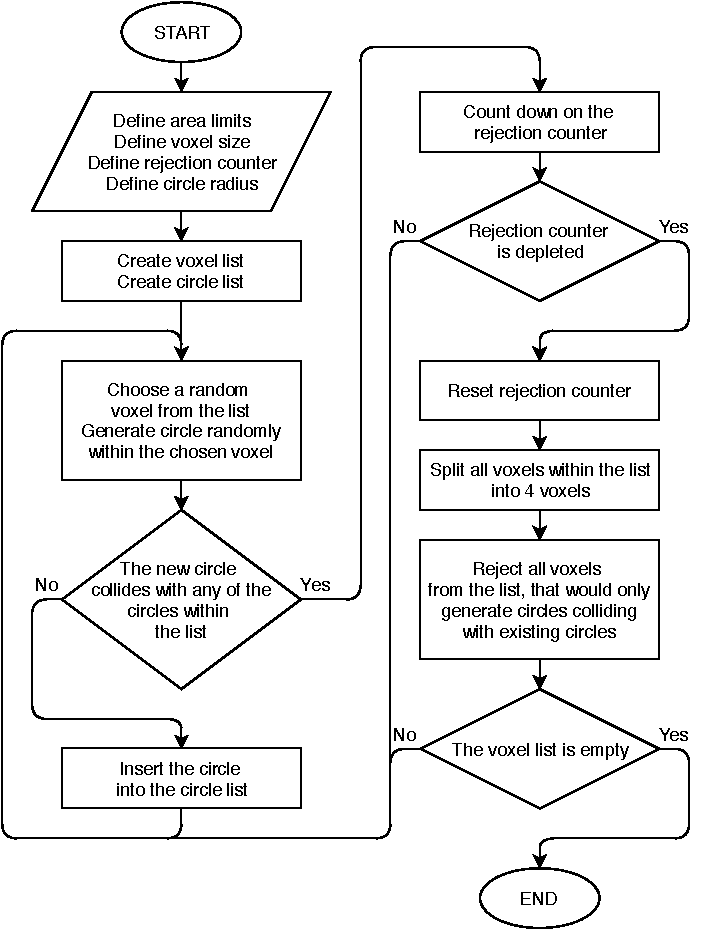
\includegraphics{Images/2dCircleRSA/VoxelCircleRSA.pdf}
  \caption{The flowchart of simple 2D RSA algorithm, using circles. \newline
		This algorithm can be expanded to remove voxels after every successful figure insertion, or to split voxels at a different condition.}

	\label{VoxelCircleRSApdff}
\end{figure}

\begin{figure}[H]
  \centering

  \begin{subfigure}[b]{0.3\linewidth}
    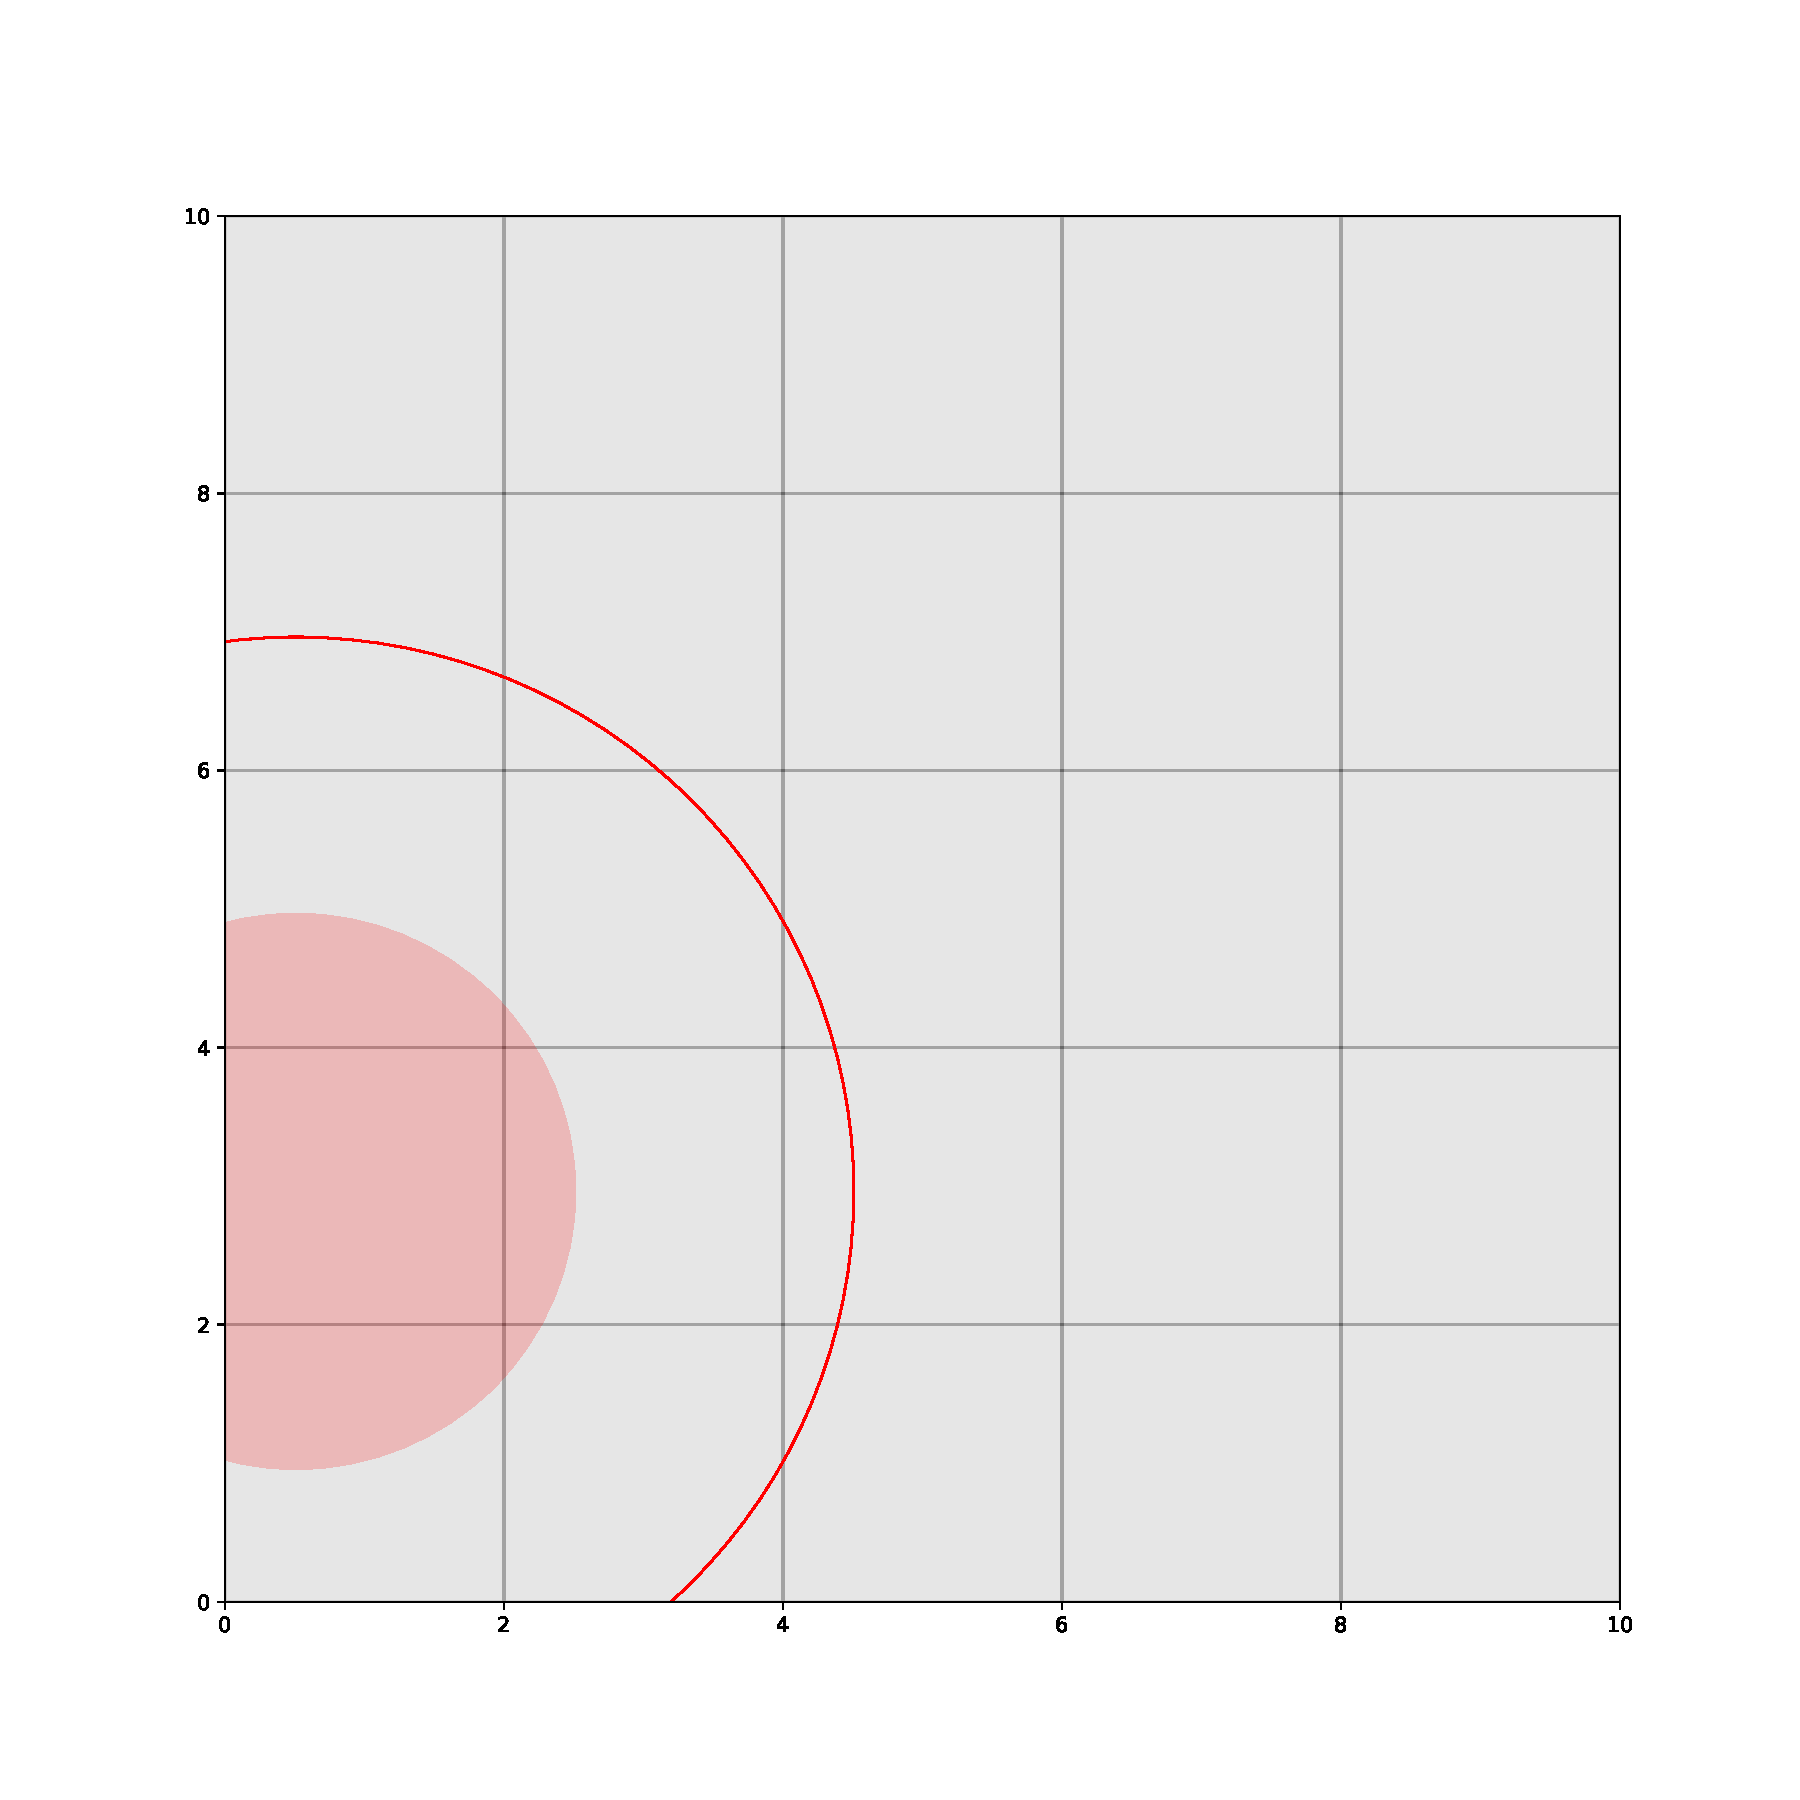
\includegraphics[width=\linewidth]{Images/2dCircleRSA/fig1.pdf}
    \caption{}
  \end{subfigure}
  \begin{subfigure}[b]{0.3\linewidth}
    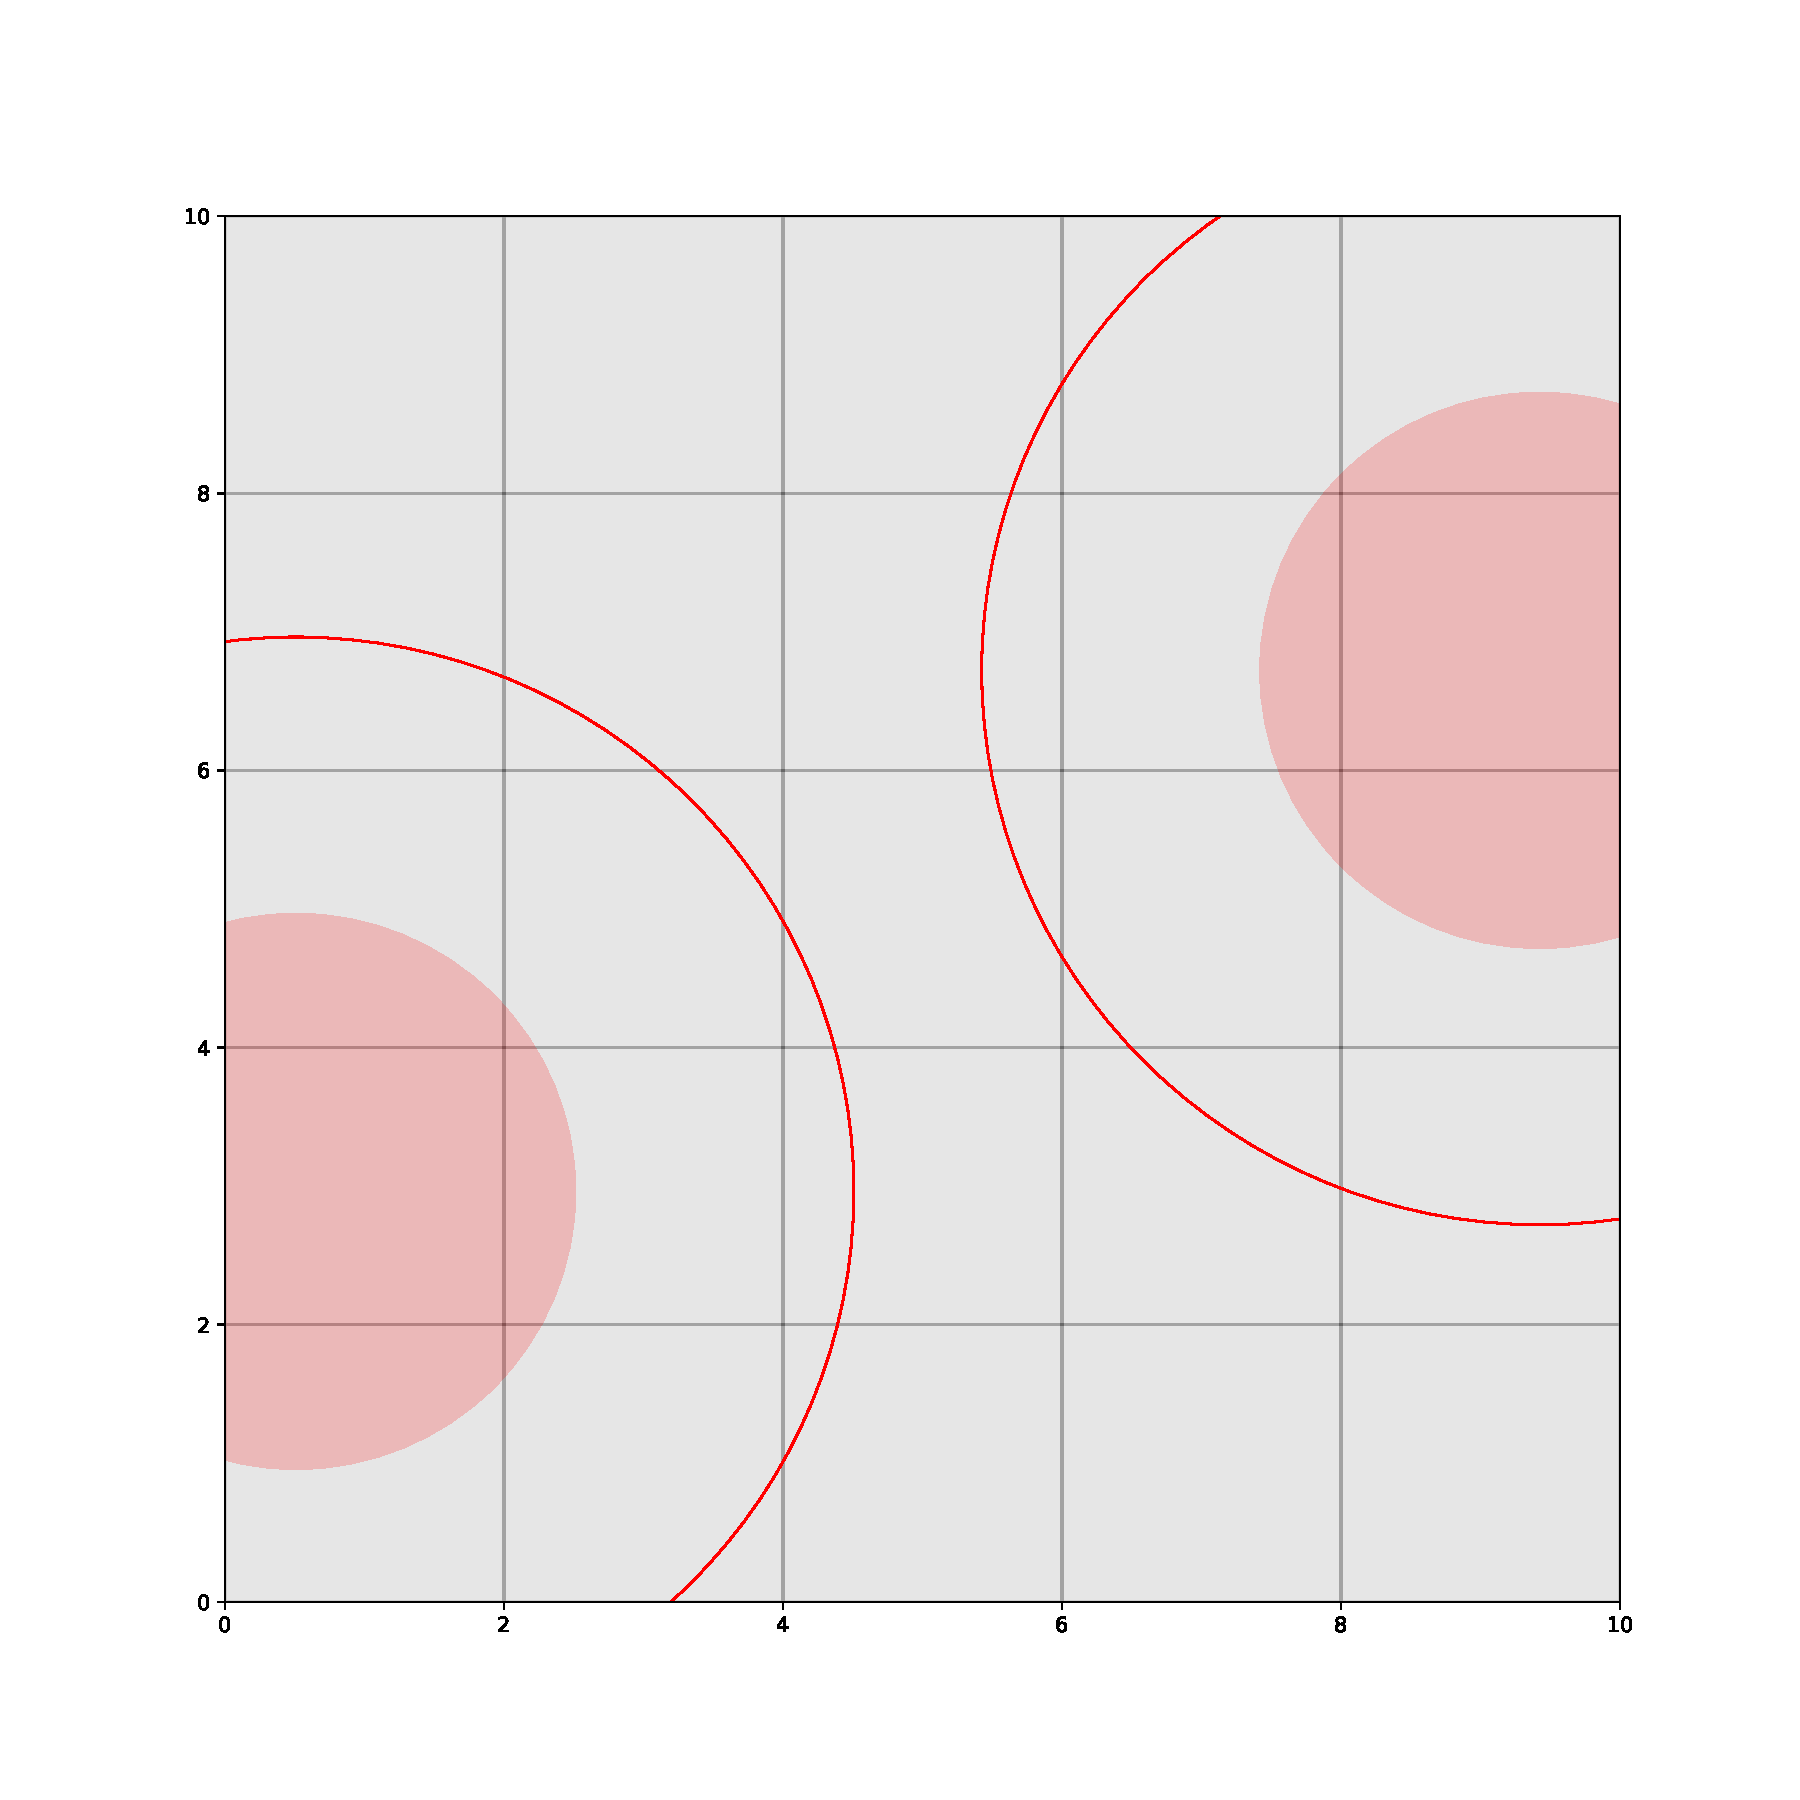
\includegraphics[width=\linewidth]{Images/2dCircleRSA/fig2.pdf}
    \caption{}
  \end{subfigure}
  \begin{subfigure}[b]{0.3\linewidth}
    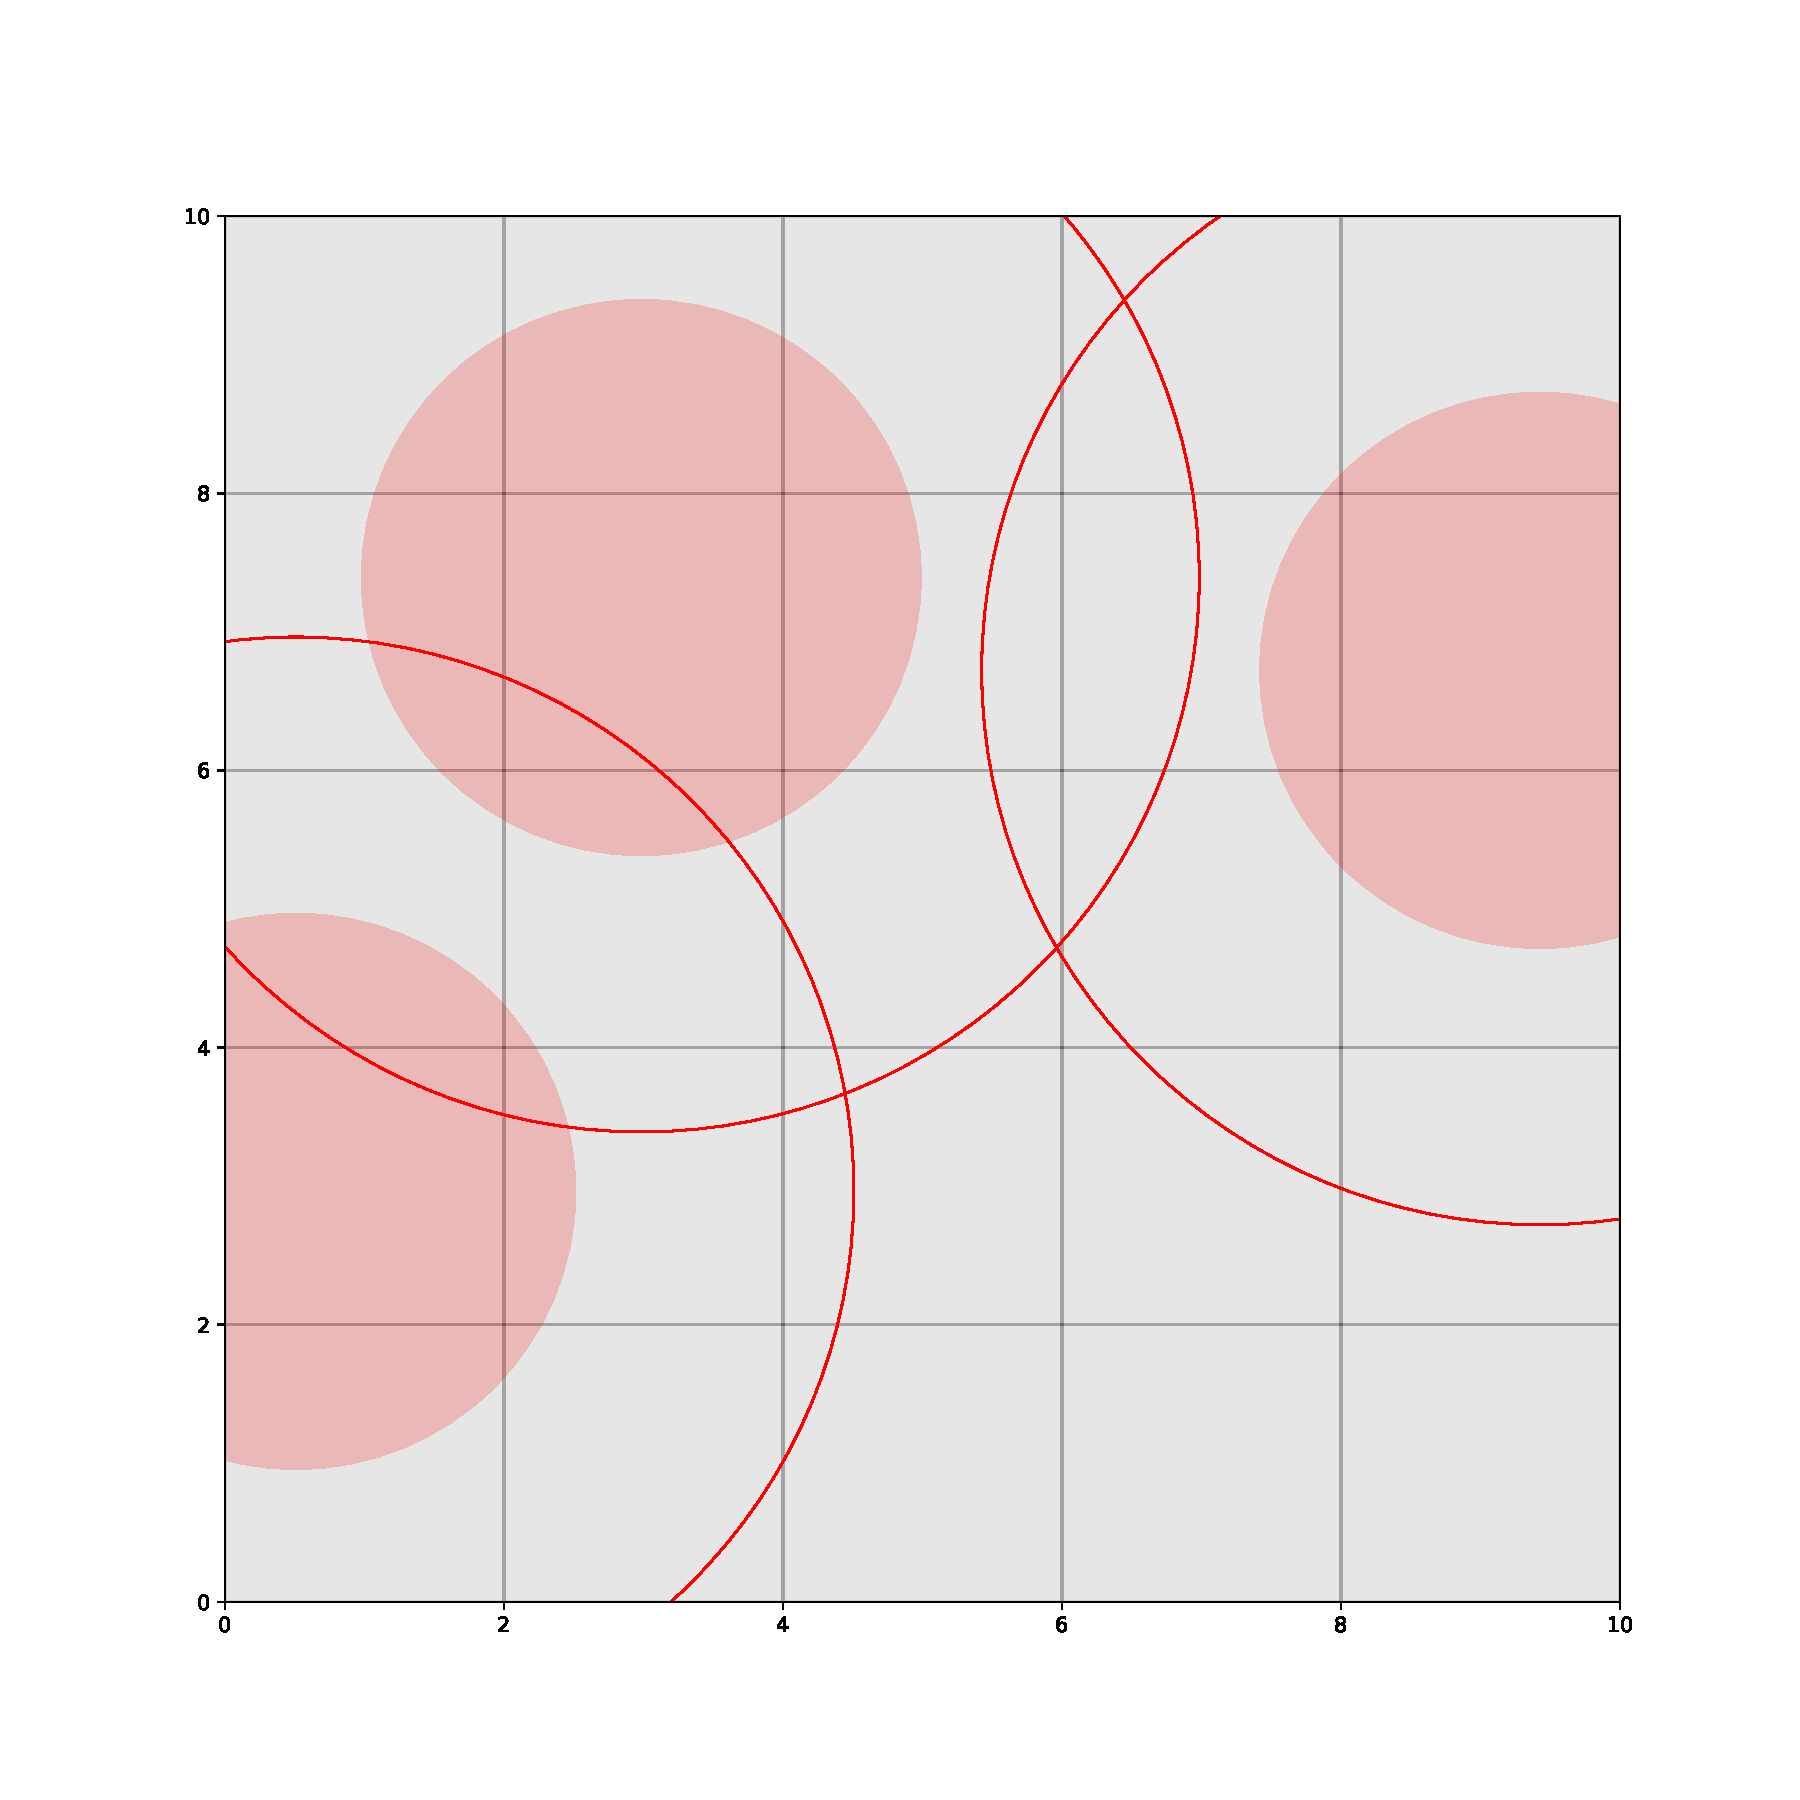
\includegraphics[width=\linewidth]{Images/2dCircleRSA/fig3.pdf}
    \caption{}
  \end{subfigure}

  \begin{subfigure}[b]{0.3\linewidth}
    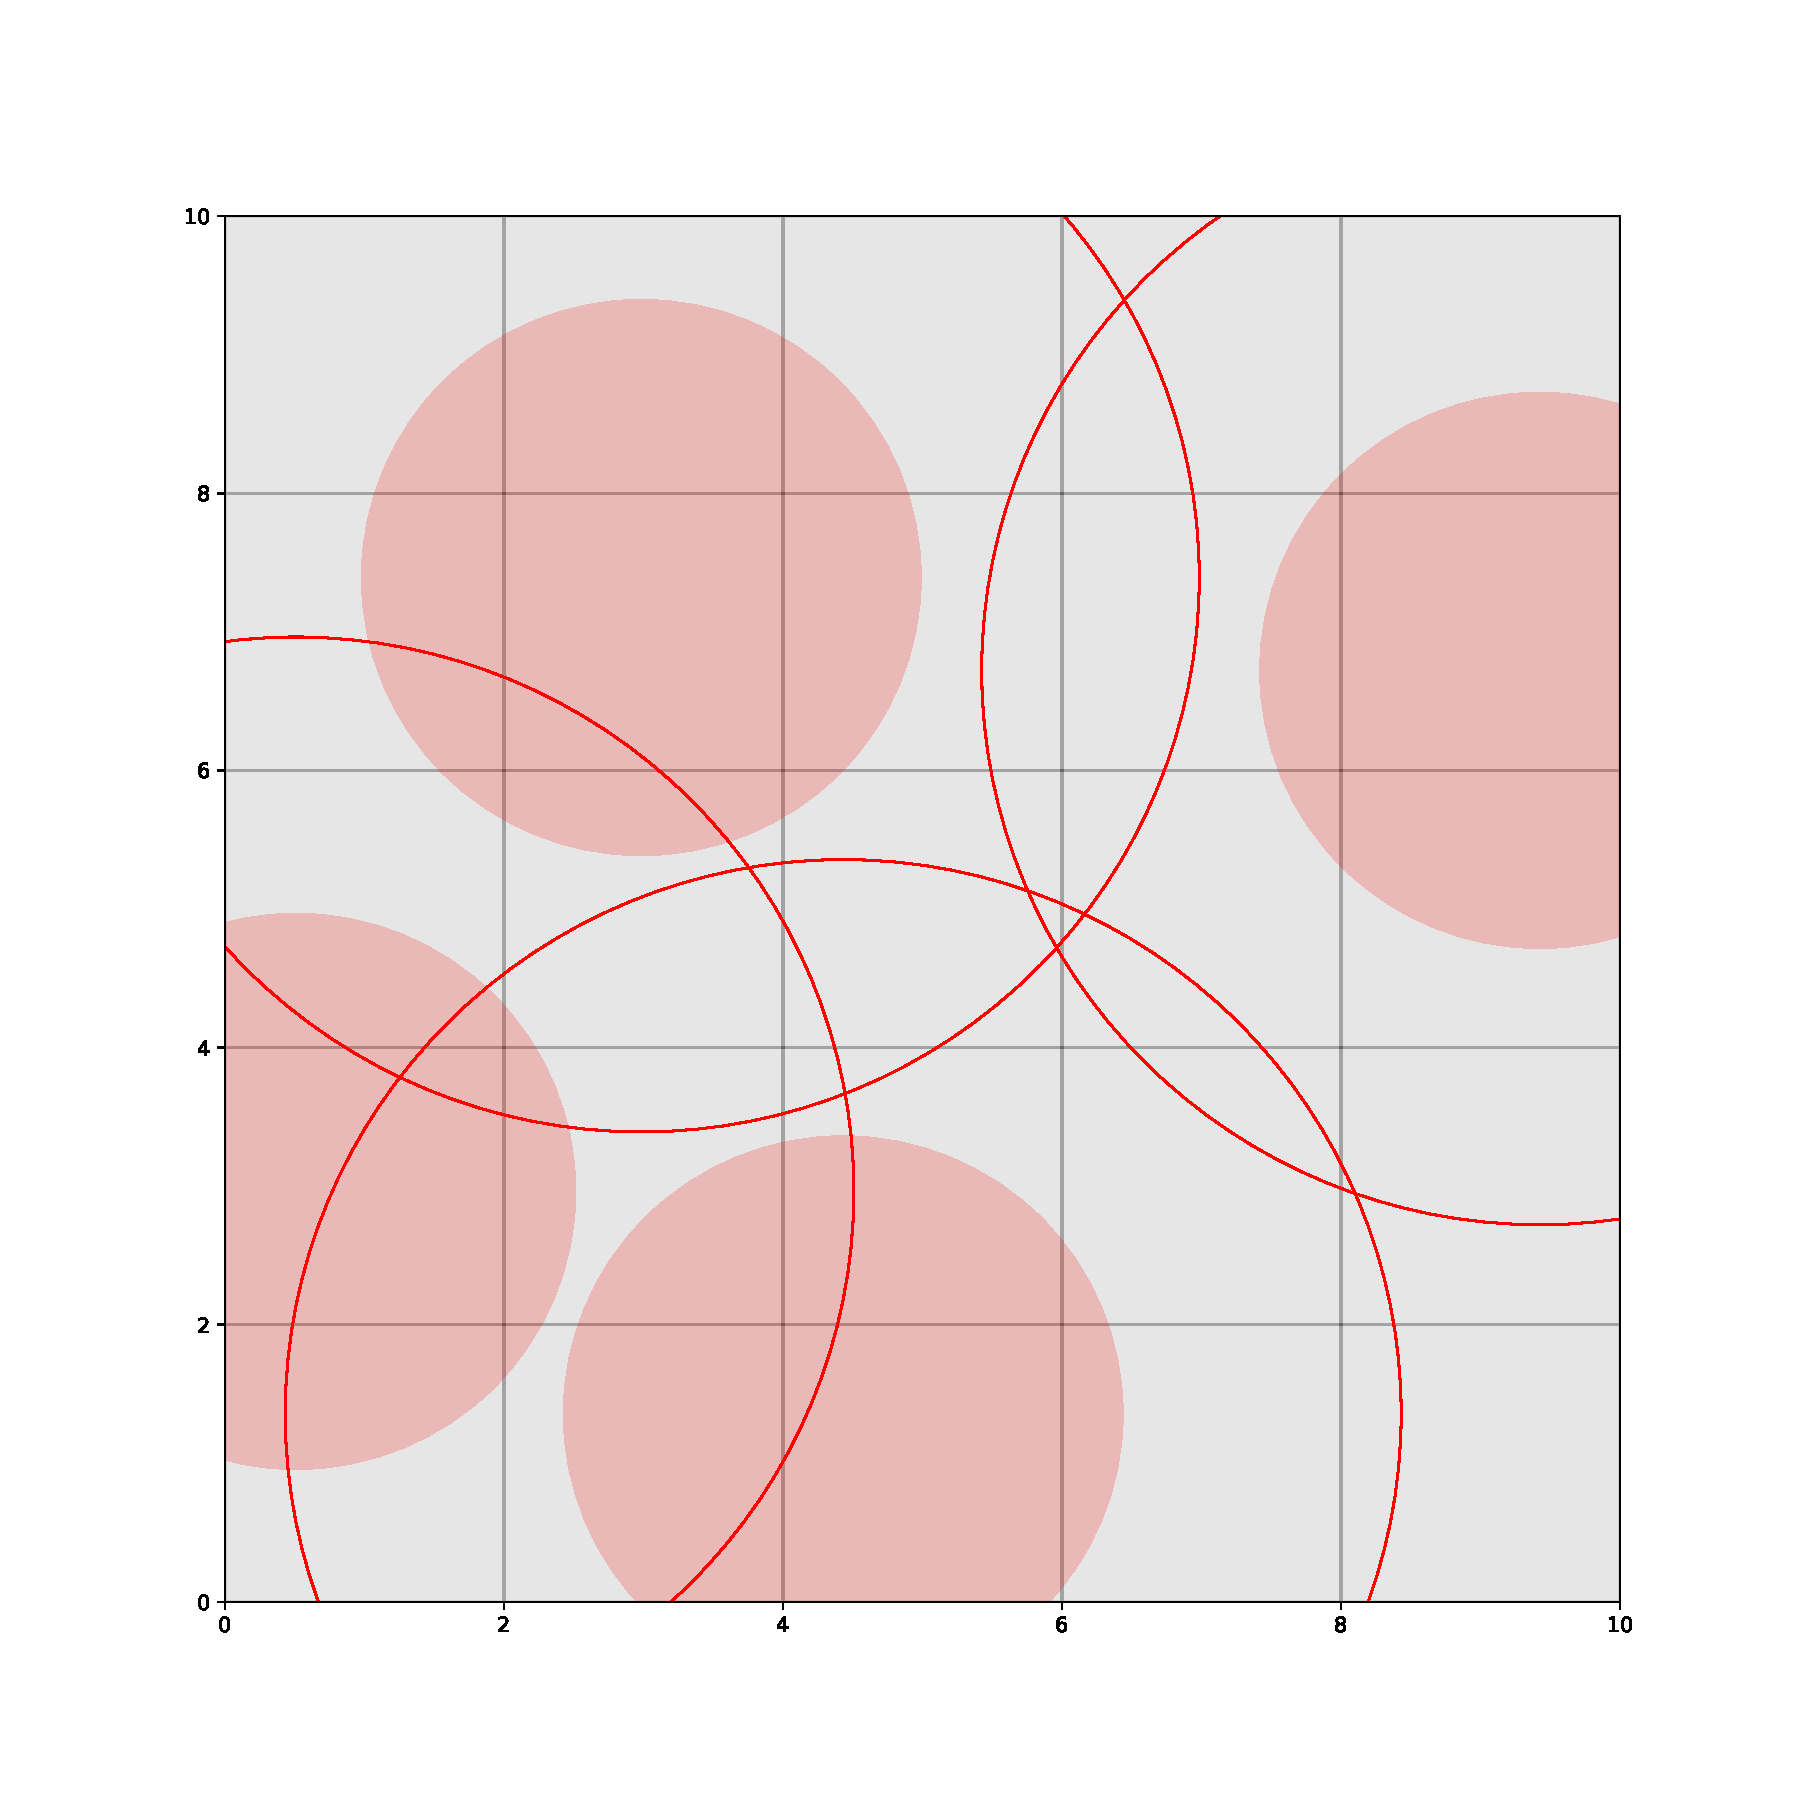
\includegraphics[width=\linewidth]{Images/2dCircleRSA/fig4.pdf}
    \caption{}
  \end{subfigure}
  \begin{subfigure}[b]{0.3\linewidth}
    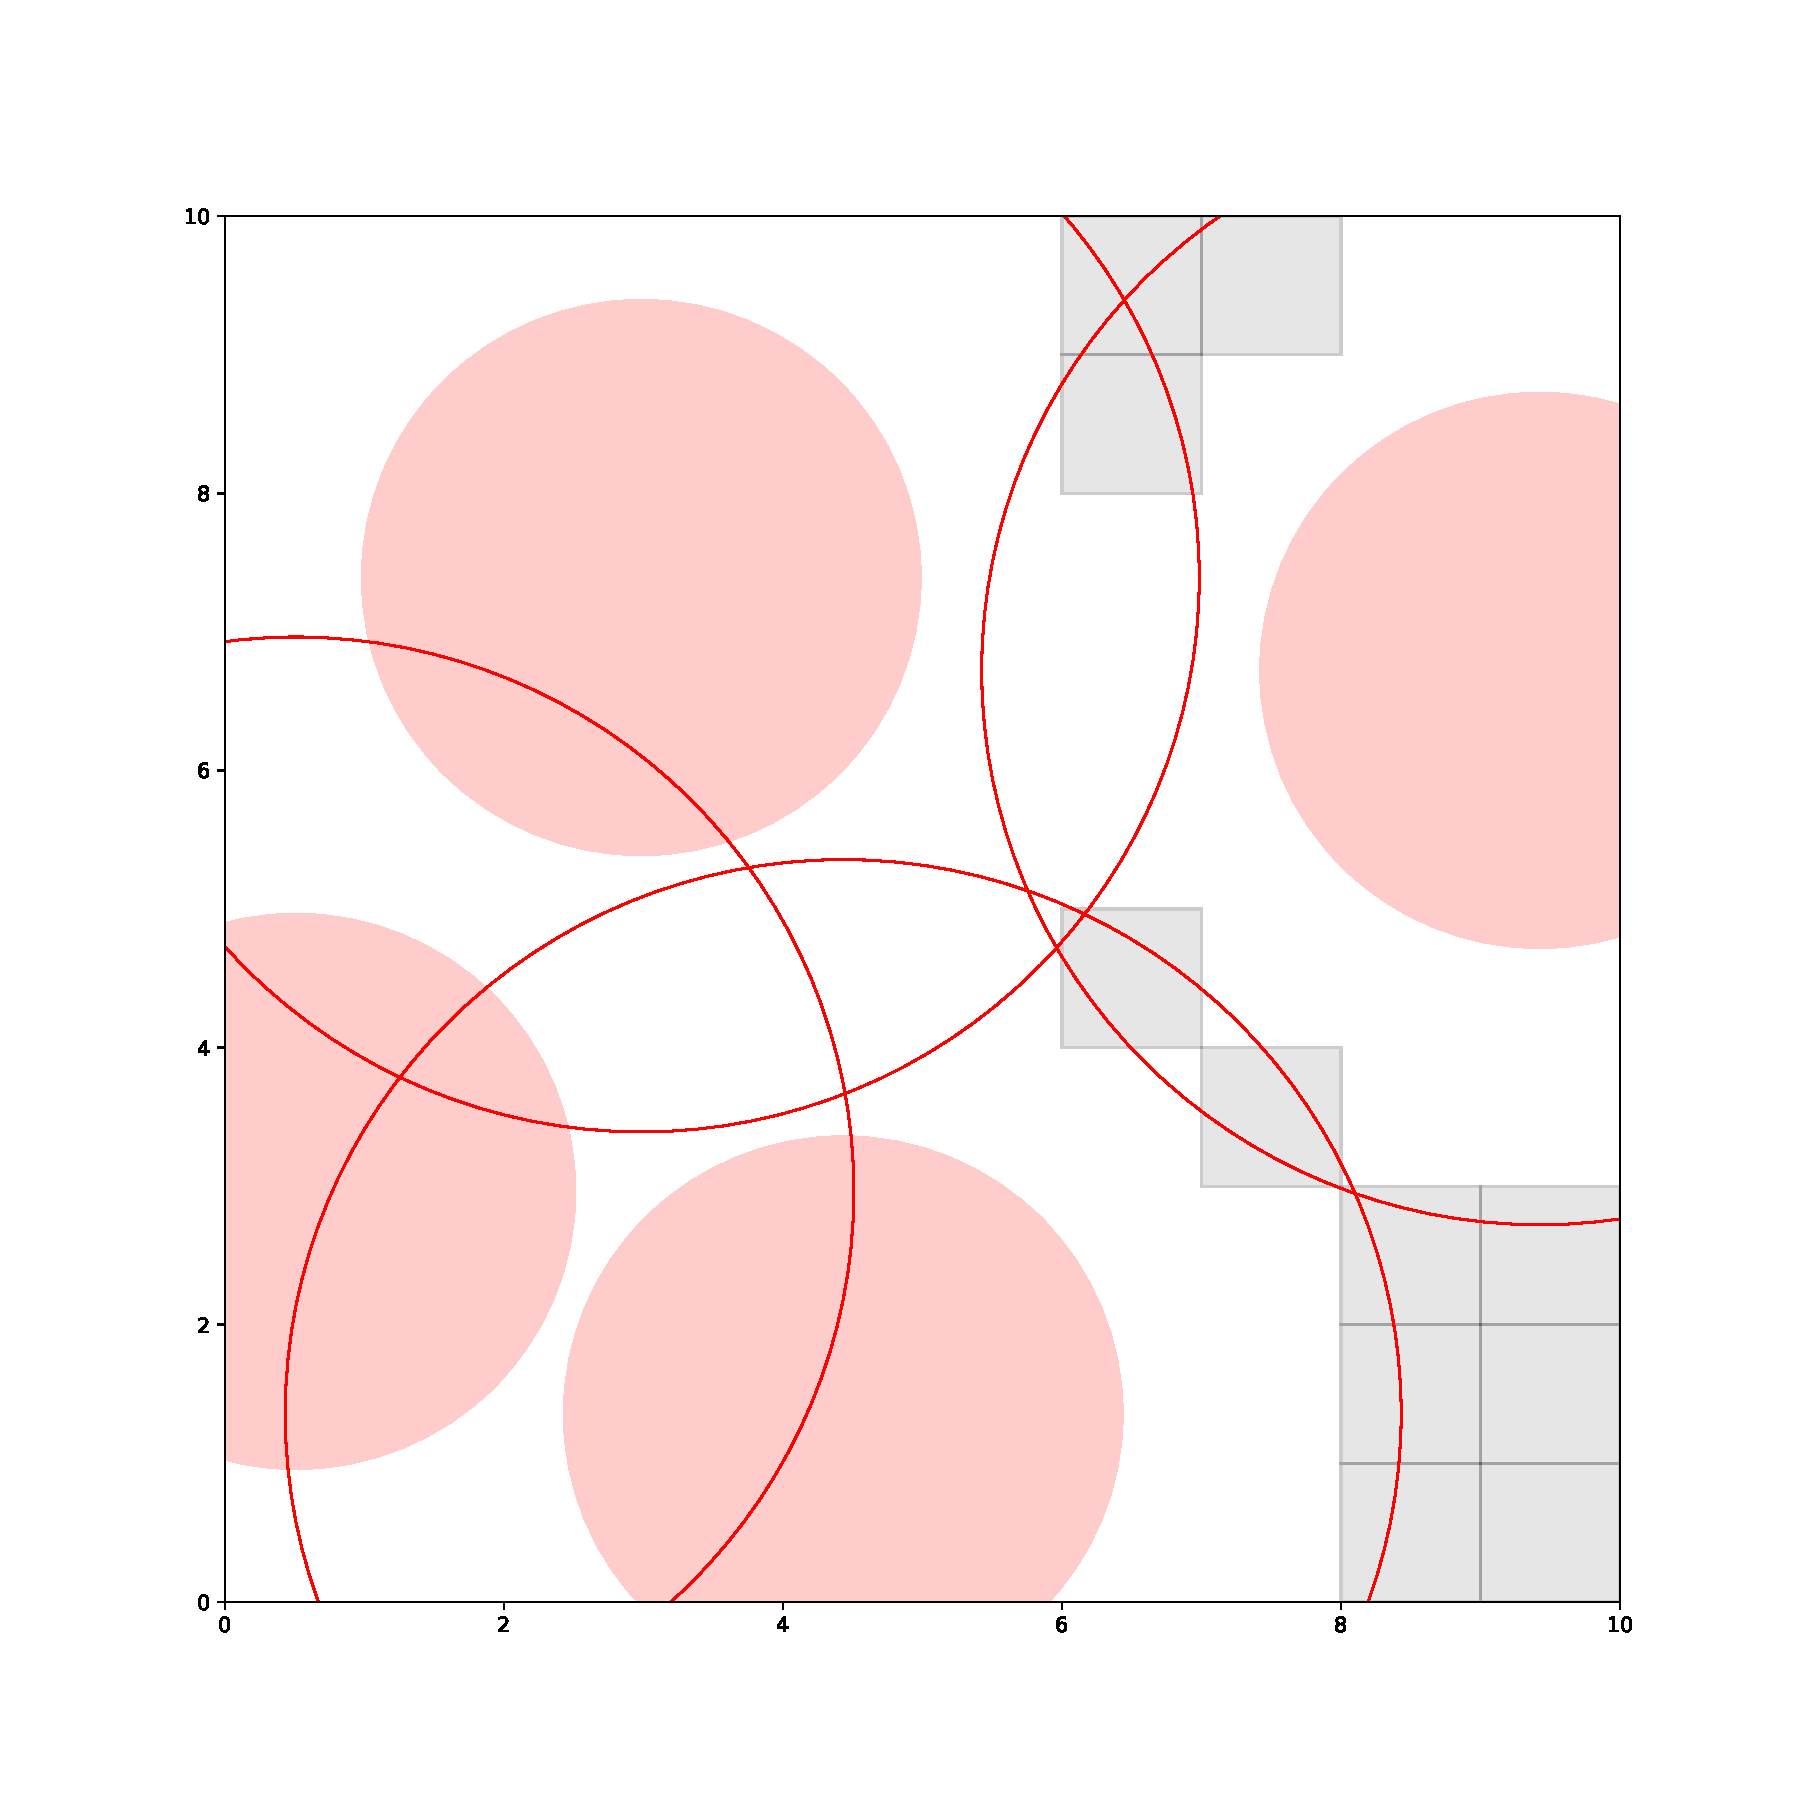
\includegraphics[width=\linewidth]{Images/2dCircleRSA/fig5.pdf}
    \caption{}
  \end{subfigure}
  \begin{subfigure}[b]{0.3\linewidth}
    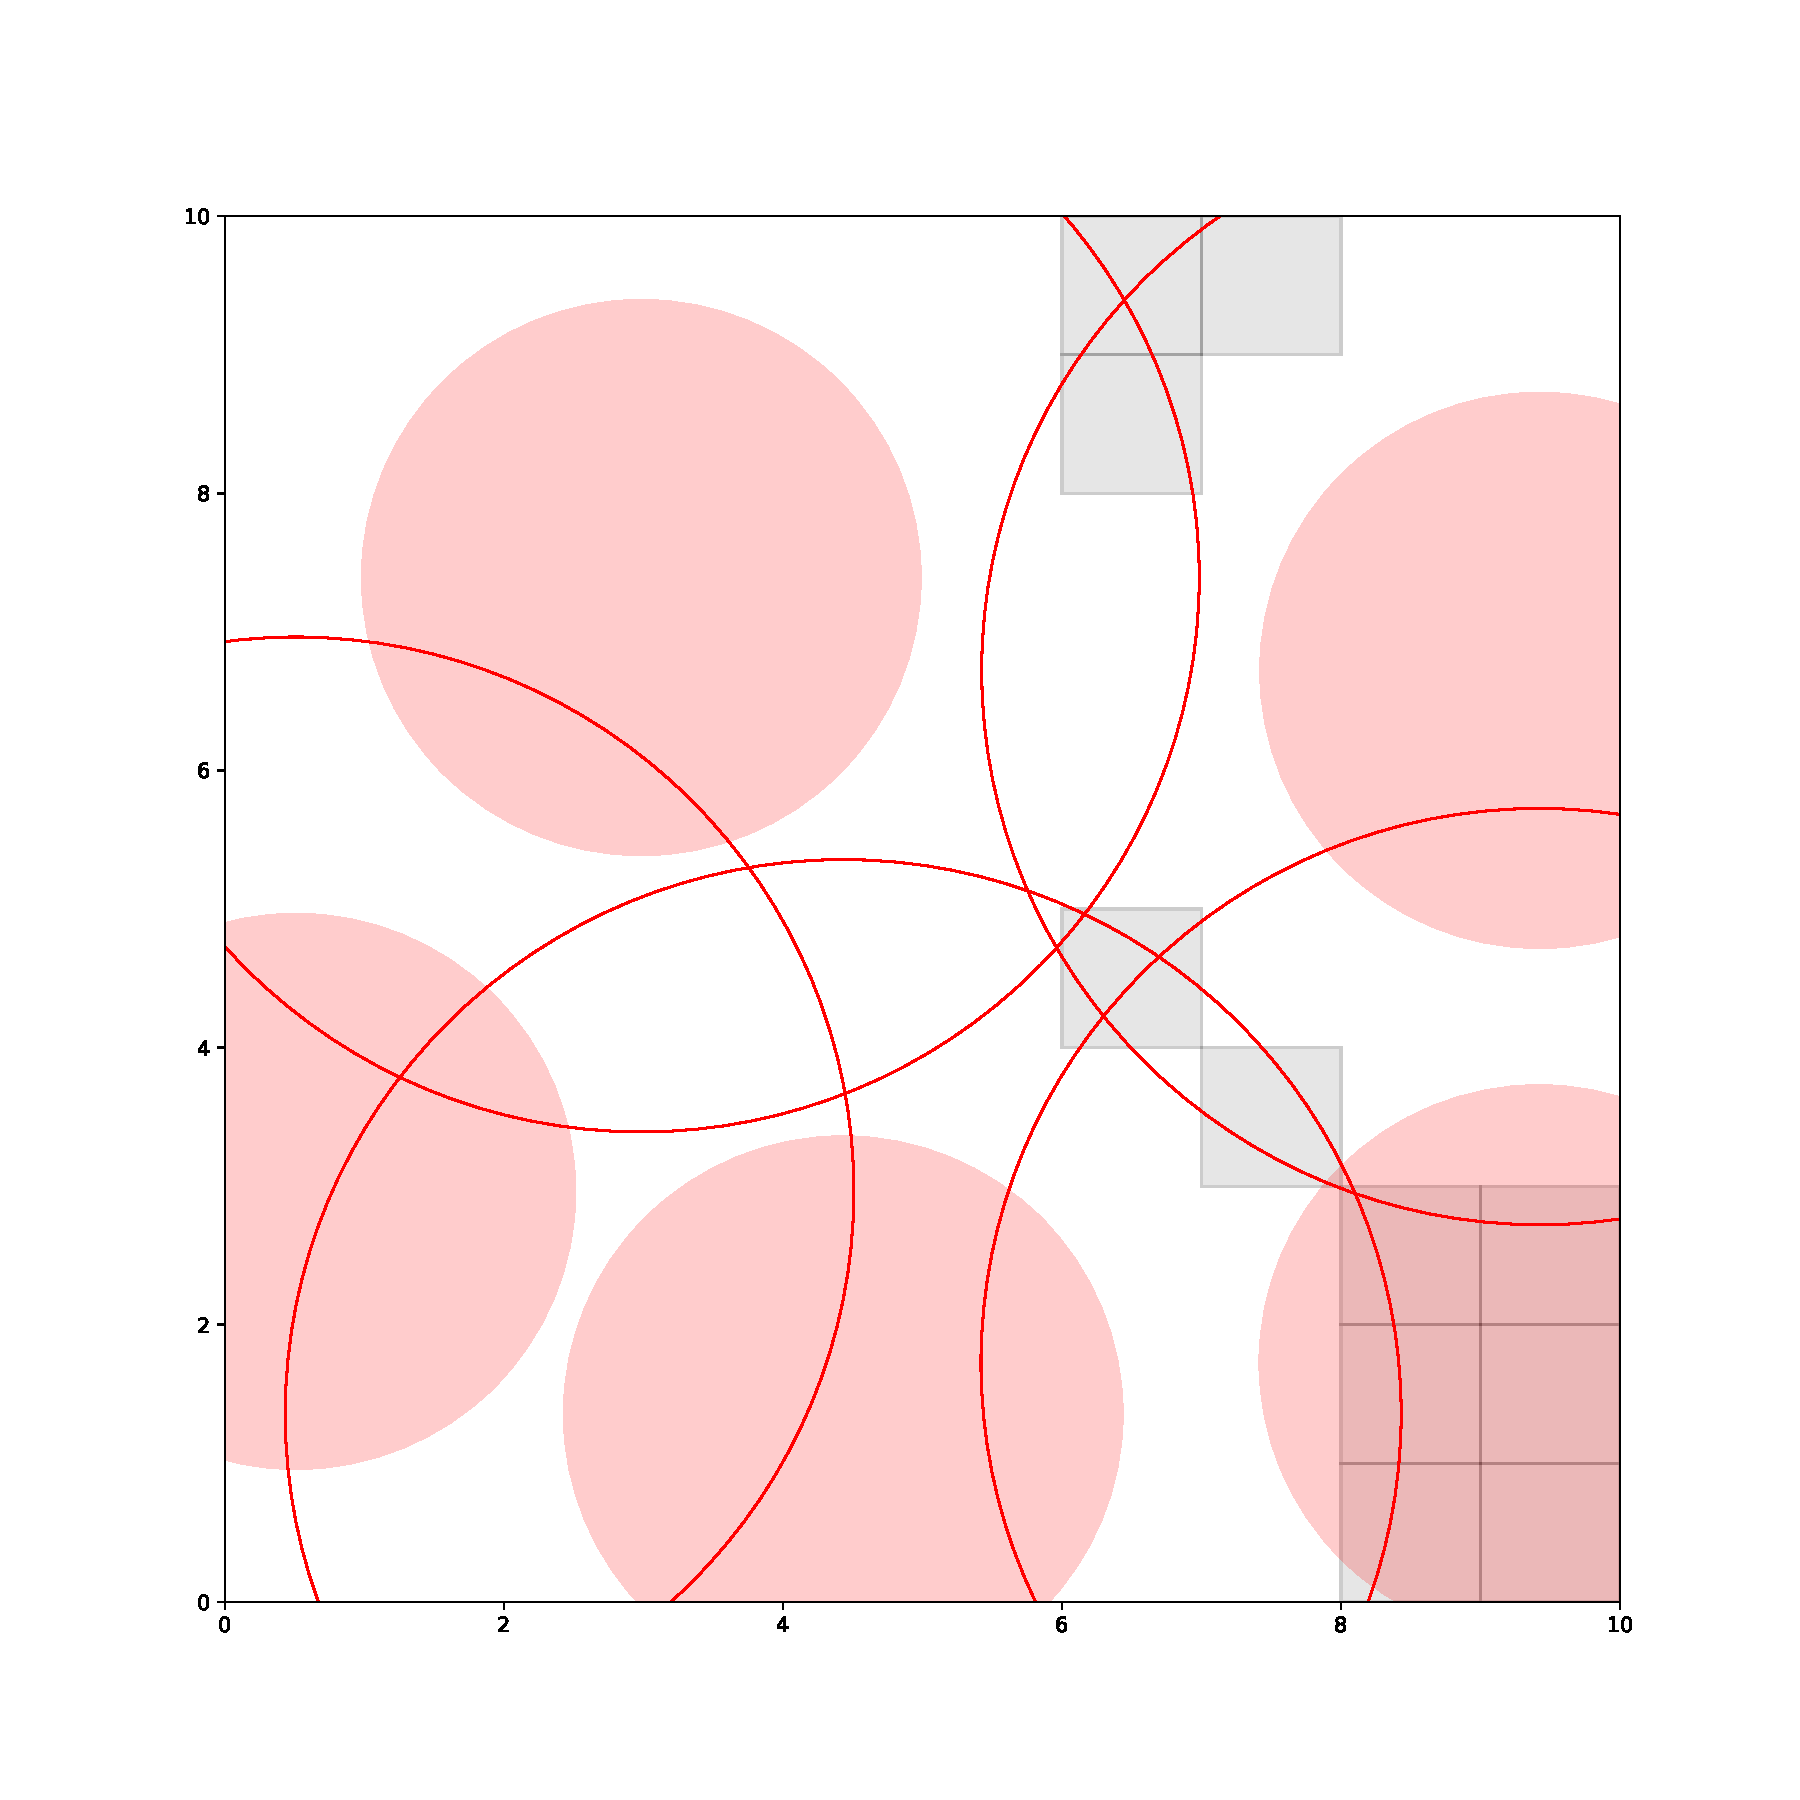
\includegraphics[width=\linewidth]{Images/2dCircleRSA/fig6.pdf}
    \caption{}
  \end{subfigure}

  \begin{subfigure}[b]{0.3\linewidth}
    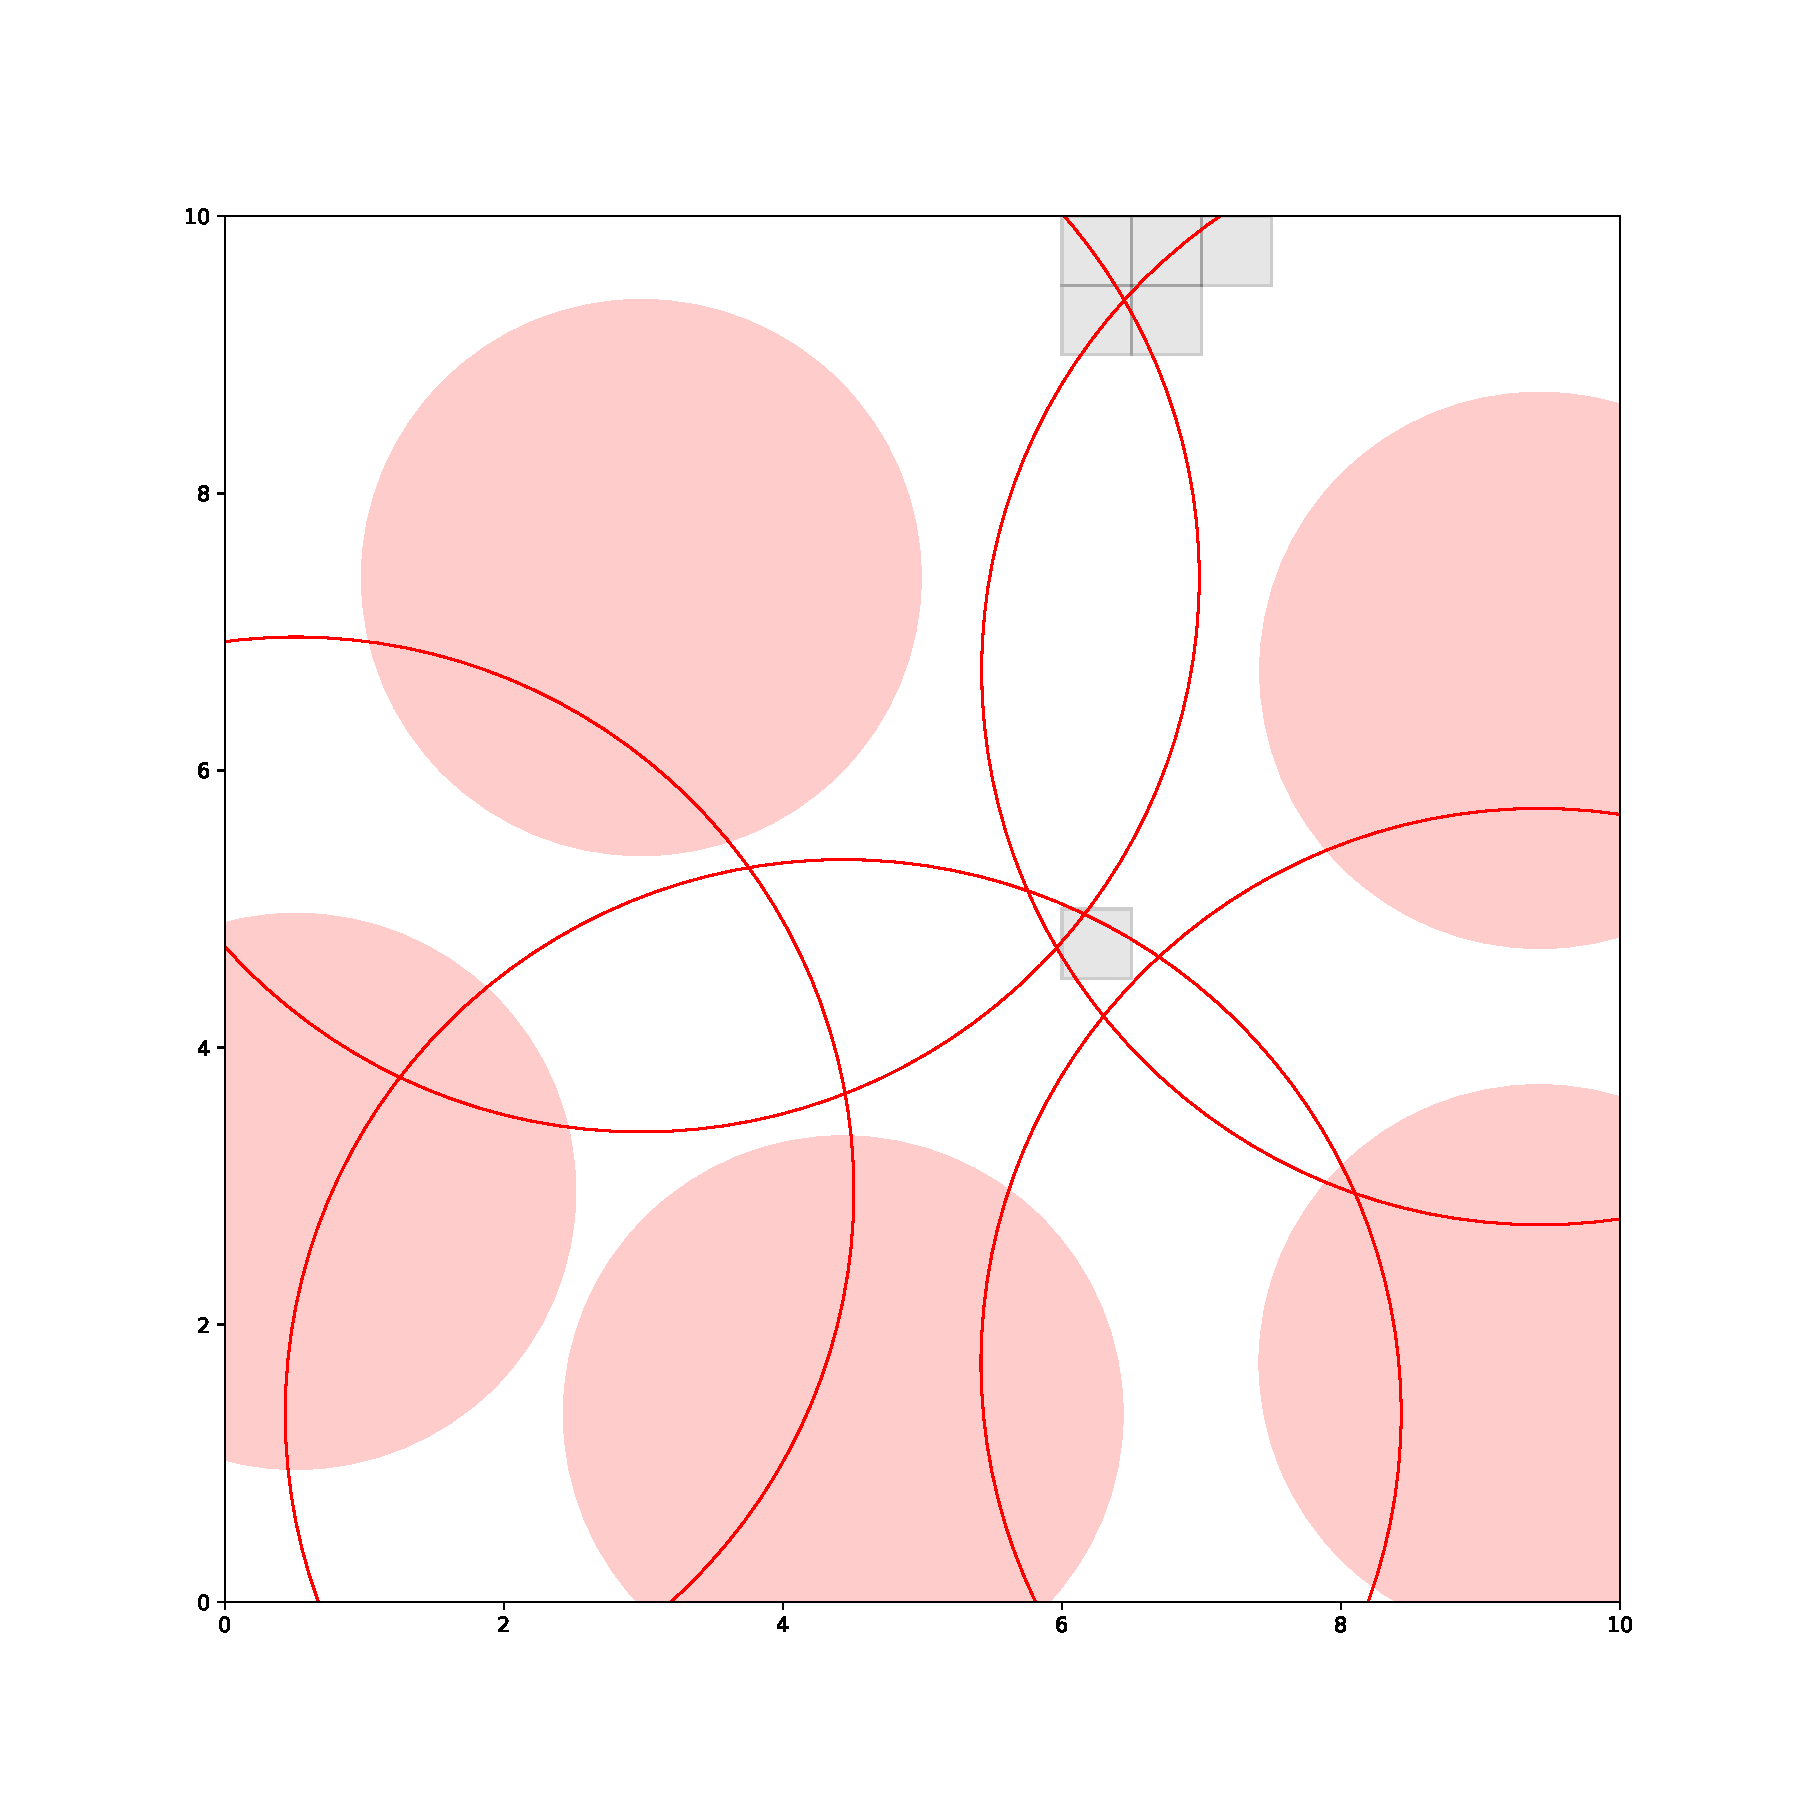
\includegraphics[width=\linewidth]{Images/2dCircleRSA/fig7.pdf}
    \caption{}
  \end{subfigure}
  \begin{subfigure}[b]{0.3\linewidth}
    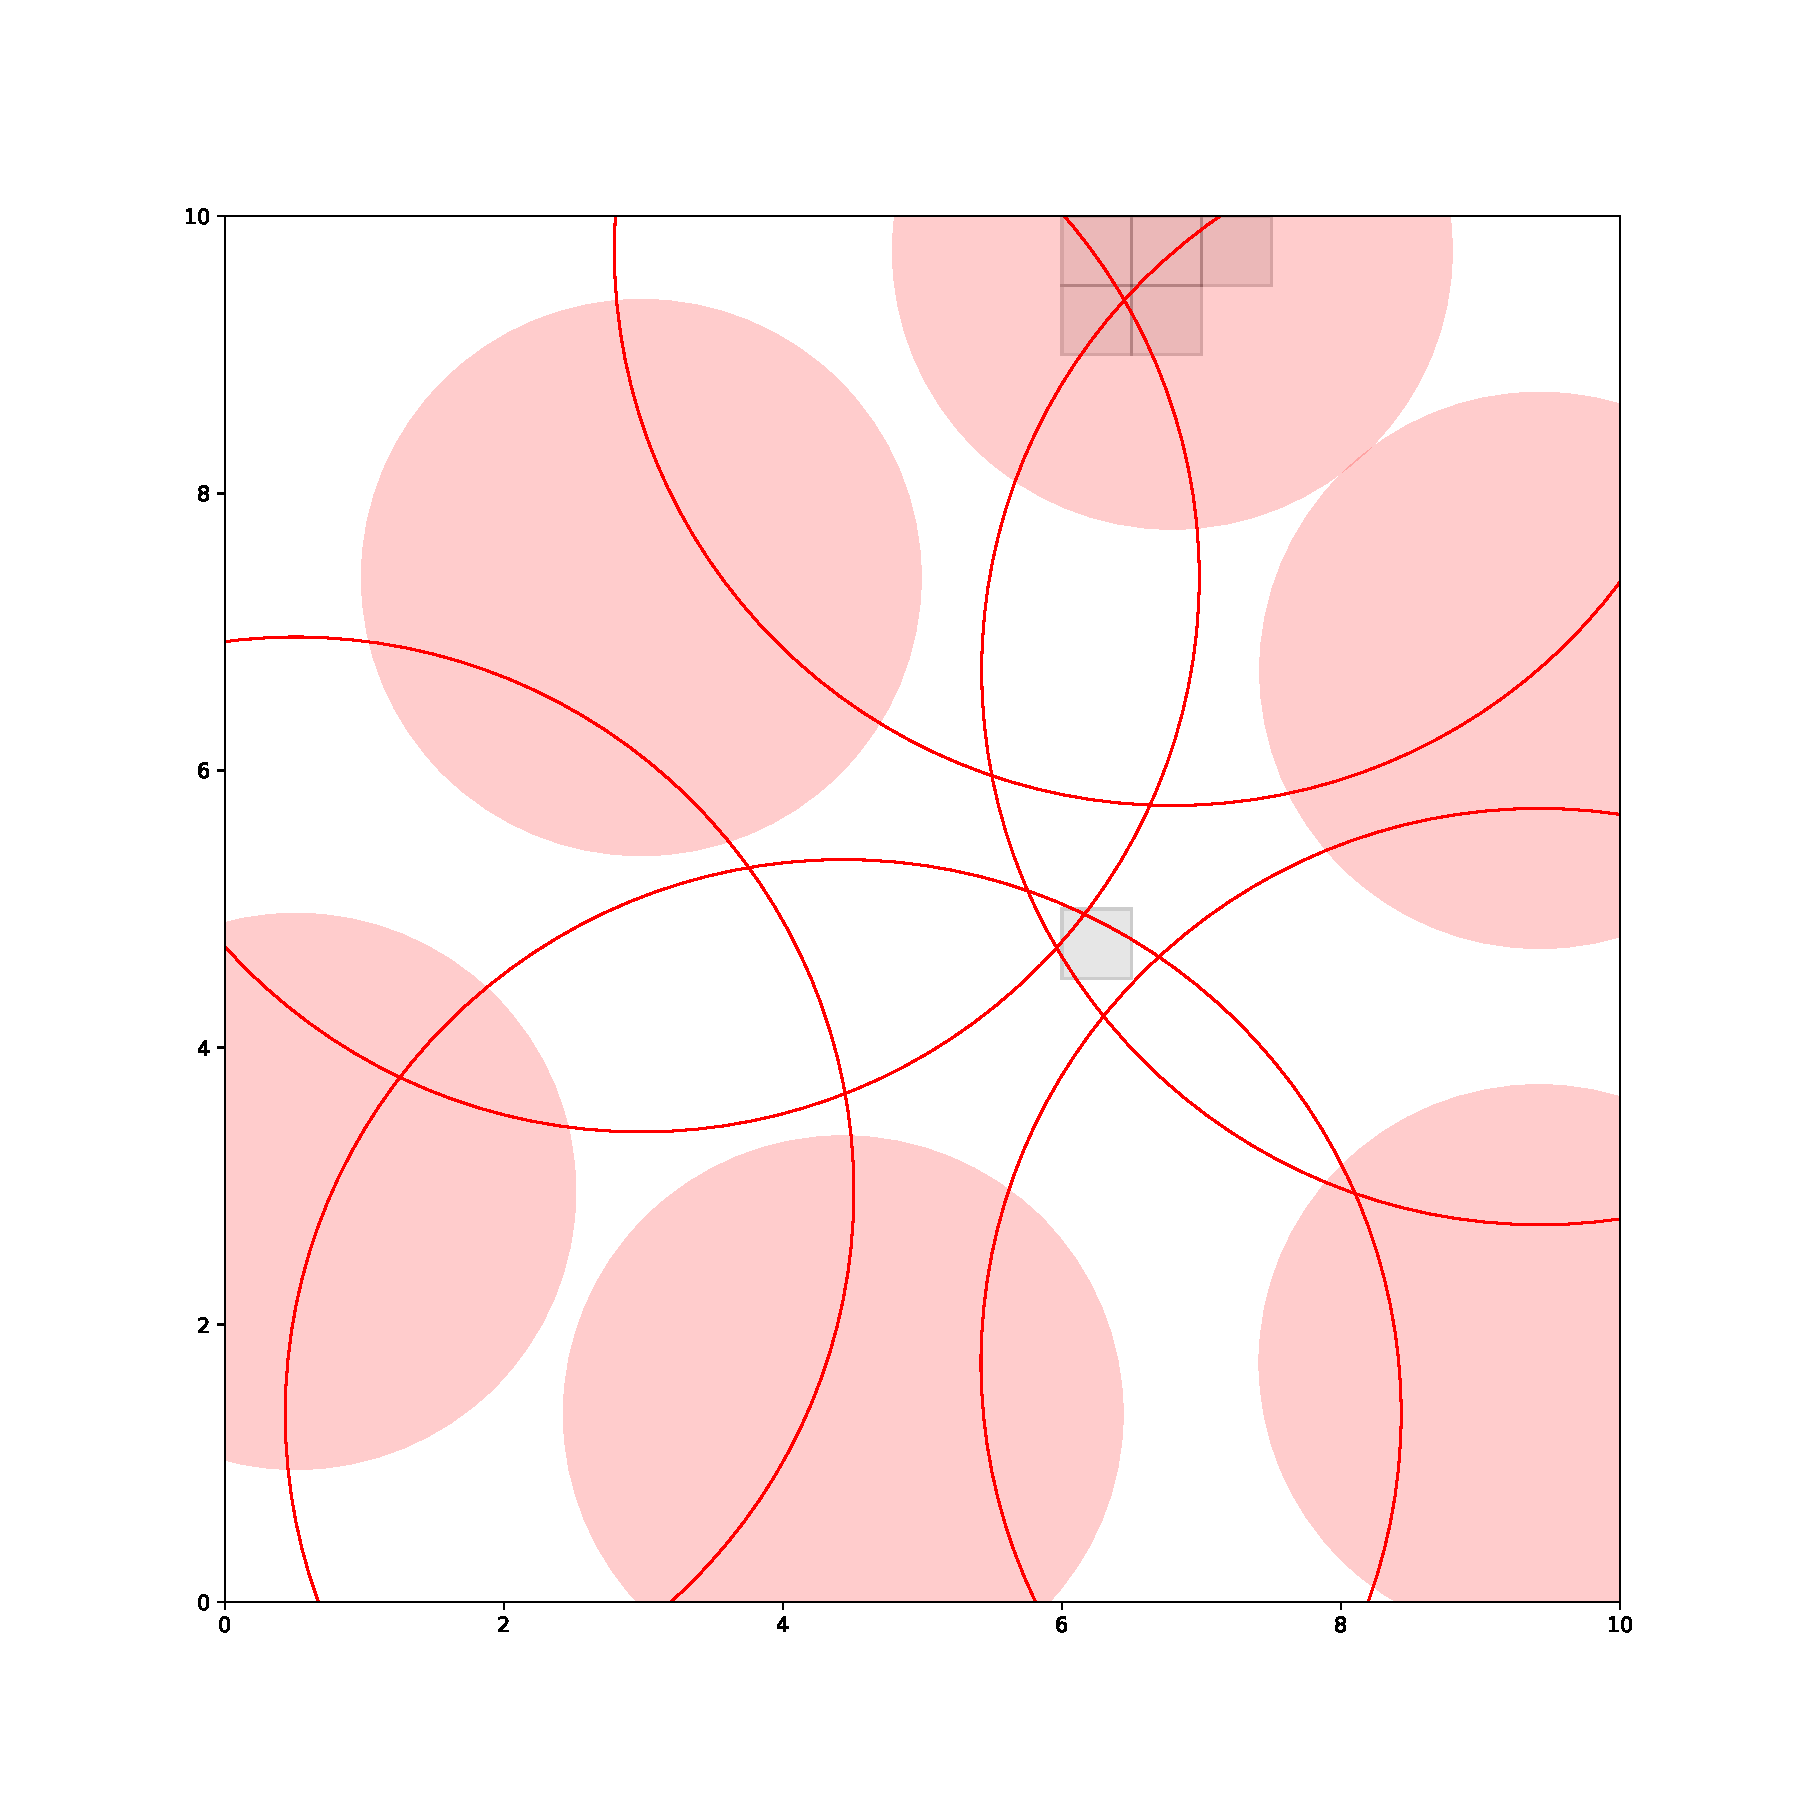
\includegraphics[width=\linewidth]{Images/2dCircleRSA/fig8.pdf}
    \caption{}
  \end{subfigure}
  \begin{subfigure}[b]{0.3\linewidth}
    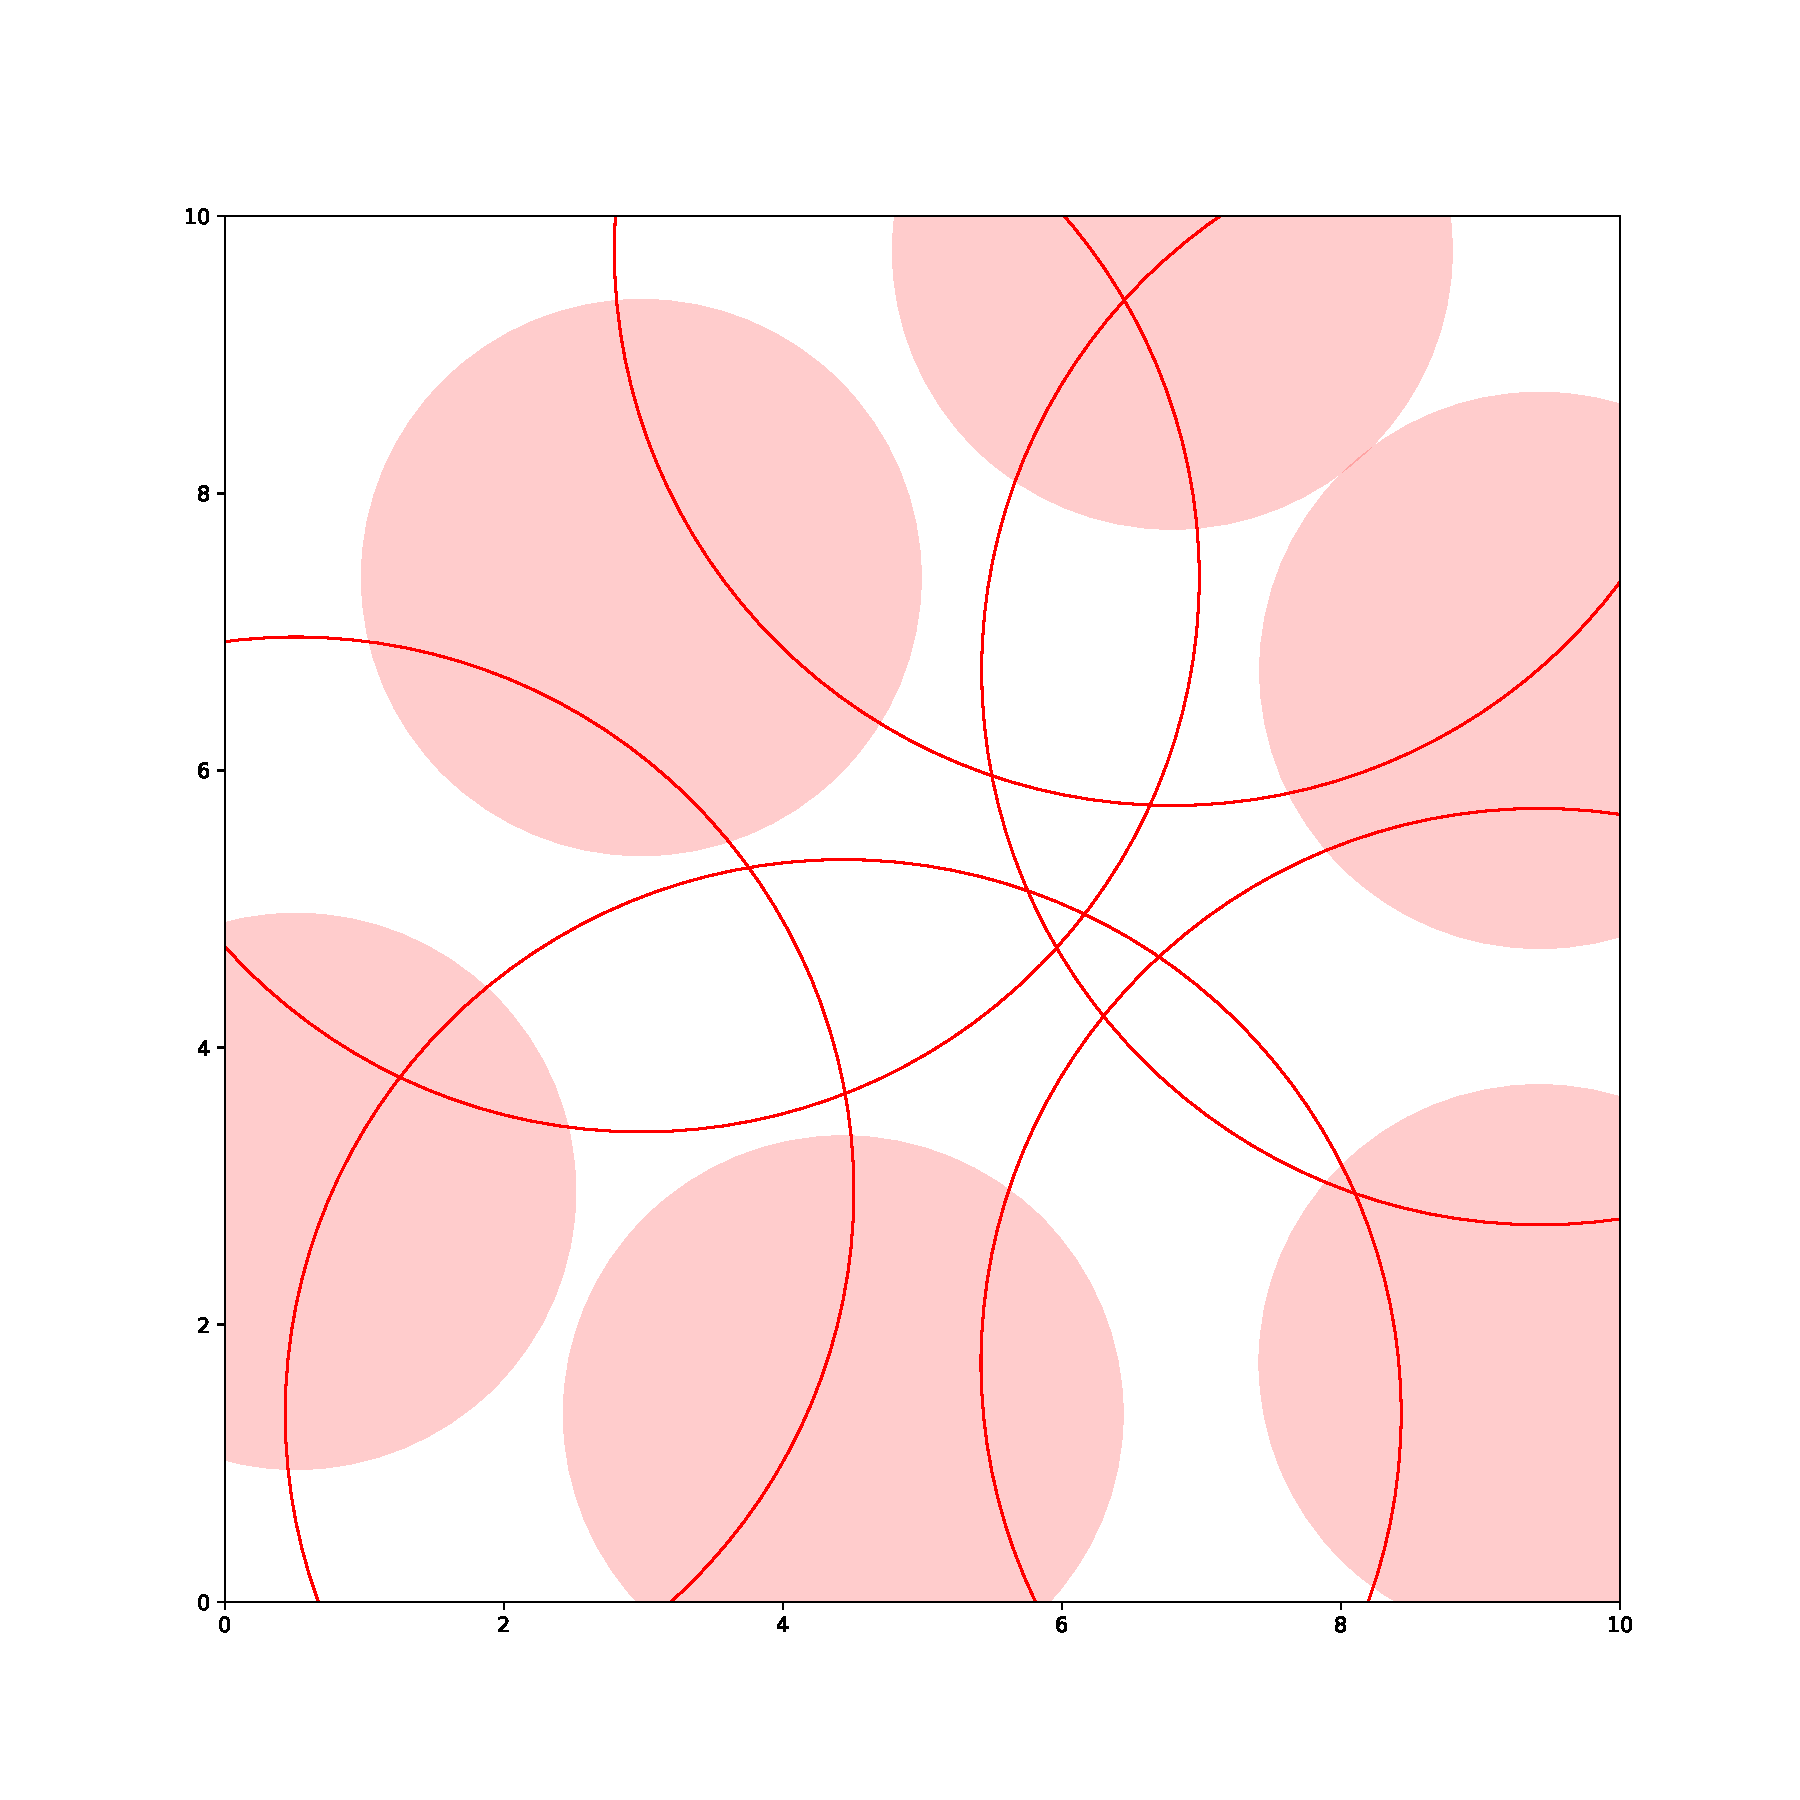
\includegraphics[width=\linewidth]{Images/2dCircleRSA/fig9.pdf}
    \caption{}
  \end{subfigure}

  \caption{The figures illustrate a simple run of the described simple 2D RSA algorithm. \newline
		The packing size is 10.0 by 10.0, the inserted circles have the radius of 2.0. The initial voxel side length is 2.0. After 10 failed attempts at inserting the circle, the voxels are split and rejected.\newline
		The figures \textit{a,b,c,d} show the insertion of the first four circles. The figure \textit{e} illustrates the effect of the voxel subdivision and rejection. Following figures illustrate next iterations of circle insertions, voxel divisions and removals, and finally, at figure \textit{i}, completely saturated system with no remaining voxels. \newline
		The voxels are rejected if they lie entirely within the double radius of any circle. In such case any new circle, with it's center within the voxel, would collide with the evaluated circle. This doubled radius is marked here as a solid red outline.}
  \label{VoxelCircleRSApdfExamples}
\end{figure}


\section {Additional Functionalities}

The previously described algorithm holds a basic structure, which is used in the expanded implementations. However, there are several features added in order to improve it's functionality and execution time. These features are listed below.

\subsection{Periodic Boundary Conditions}

The Periodic Boundary Conditions is a special behavior of the packing space. If a shape is placed nearby the edge of given space, the shapes placed at the opposite edge collide with it. They behave as if the opposite edge of the space would be a continuation of this edge. The periodic boundary conditions serve to improve packing efficiency, and remove edge-related artifacts. In essence, the periodic boundary conditions 'simulate' an infinite area, and thus may be helpful to model surfaces of greater area than the provided space \cite{ciesla_mziff}.

\begin{figure}[H]
  \centering

  \begin{subfigure}[b]{0.4\linewidth}
    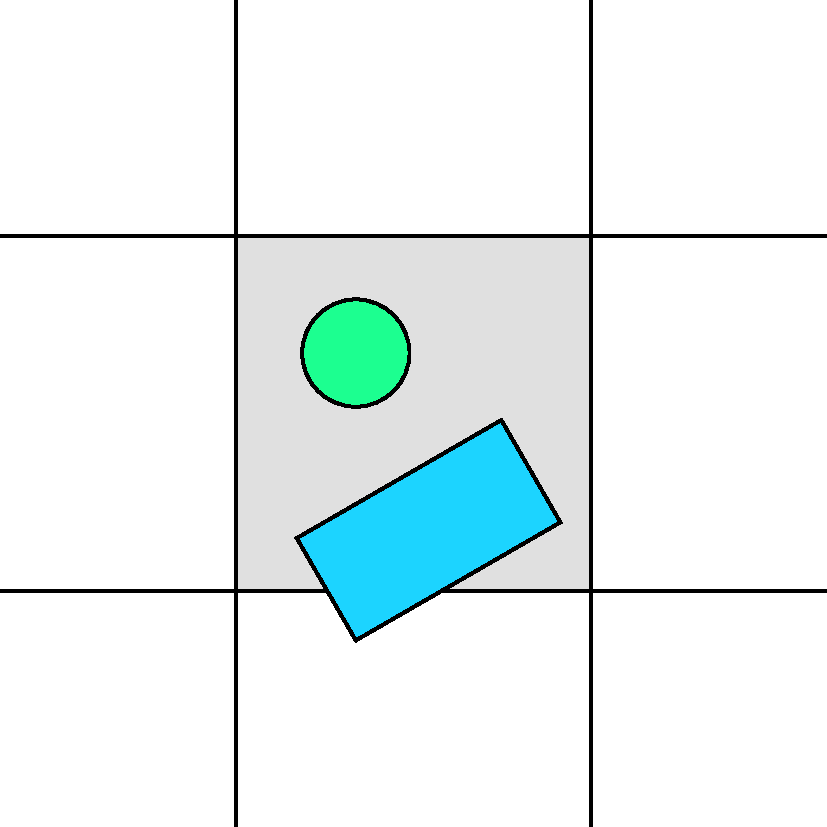
\includegraphics[width=\linewidth,height=\linewidth]{Images/CieslaAlgorithm/pec1.pdf}
    \caption{Without the periodic boundary conditions}
  \end{subfigure}
  \begin{subfigure}[b]{0.4\linewidth}
    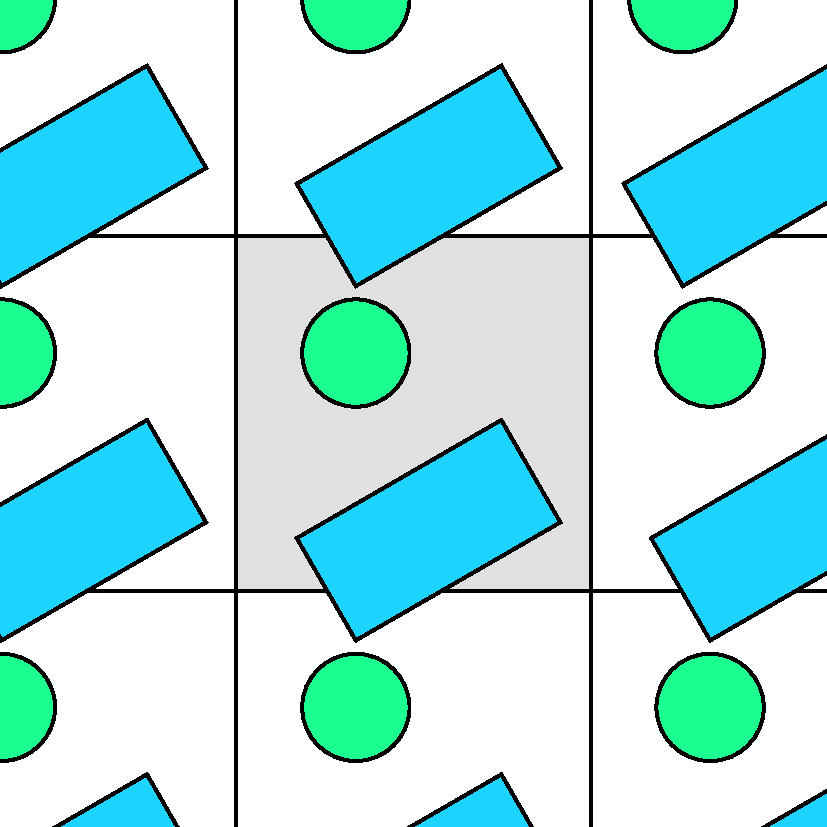
\includegraphics[width=\linewidth,height=\linewidth]{Images/CieslaAlgorithm/pec2.pdf}
    \caption{With the periodic boundary conditions}
  \end{subfigure}

\caption{The figure demonstrates the function of periodic boundary conditions, on a square space.}
\end{figure}

\subsection{Adjacency Matrix}

During the execution of the algorithm, the function determining if two shapes collide, is executed at two points. First, when the shape is inserted, it is determined if it collides with any already existing shape. The second time, it is when the voxel is rejected - it must be checked against all shapes, until one that would cause it's rejection is found. \newline
It is possible to limit the executions of these functions to a far lesser number. The space can be divided into a number of rectangular cells, containing shapes and voxels. It is then only necessary to check collisions between the shapes that belong to the same, or neighboring cells, to determine if they overlap each other. The minimal width of the cell must be equal to the radius of the shape's minimal bounding cirlce. \newline
Also, the periodic boundary conditions can be easily implemented using this solution. The content of cells from one edge can be referenced while investigating the opposite edge of the space.


\begin{figure}[H]
  \centering

  \begin{subfigure}[b]{0.4\linewidth}
    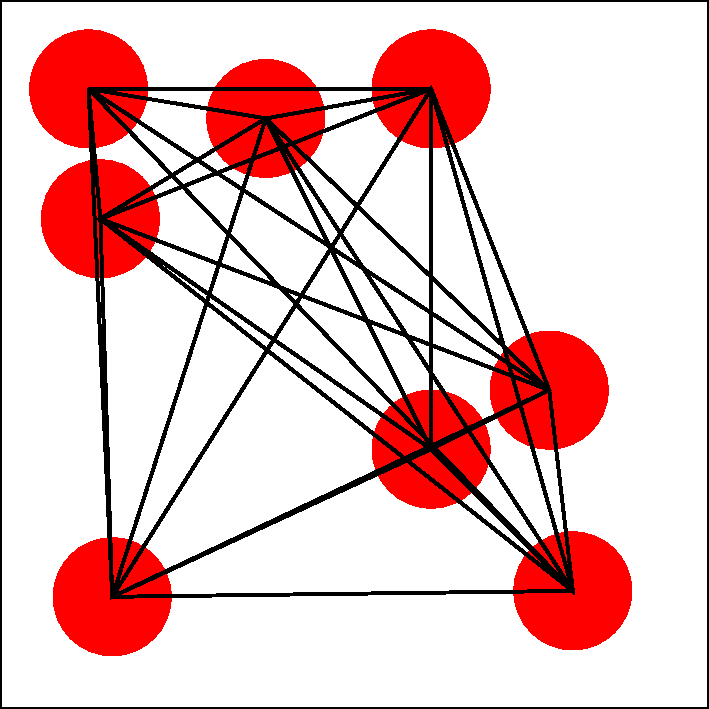
\includegraphics[width=\linewidth,height=\linewidth]{Images/CieslaAlgorithm/adjmatrix0.pdf}
    \caption{}
		\label{adjmatrix_label0}
  \end{subfigure}
  \begin{subfigure}[b]{0.4\linewidth}
    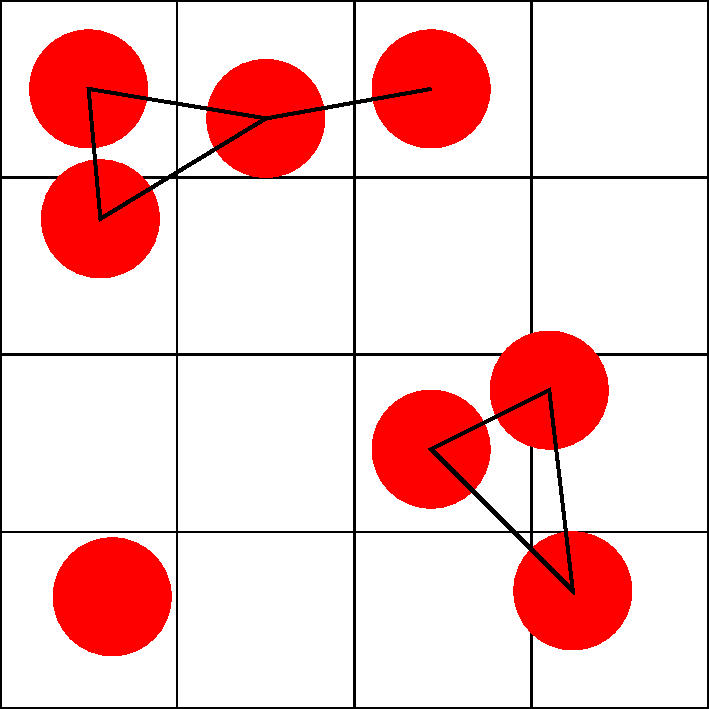
\includegraphics[width=\linewidth,height=\linewidth]{Images/CieslaAlgorithm/adjmatrix1.pdf}
    \caption{}
		\label{adjmatrix_label1}
  \end{subfigure}

\caption{The figures demonstrate the collision checks performed on a set of shapes with (\textit{b}) and without (\textit{a}) an adjacency matrix. The collision checks are represented by lines connecting the circle centers. The circle belongs to a cell, if it's center lies within it.}
\end{figure}

\subsection{Polydisk Shape Collision}

The algorithm uses a shape, consisting of a list of disks with given radiuses, and a relative position to an arbitrary center. It is relatively easy to check if two such shapes collide. \newline
If two disks collide, the distance between their centers is lesser or equal to the sum of their radiuses. Two polydisks will overlap, if any of the circles within one of them, will collide with any circle of the other.

\subsection{Polydisk Voxel Rejection}

The much more complex problem is the voxel rejection. The first issue is that since the shapes can have a different angle, this needs to be implemented in the voxel's structure - the solution was to add a third dimension, representing the available angles in which the shapes may appear. \newline \newline
The voxel is rejected if no new shapes can be inserted within it, at any position or angle. This happens if there exists at least one shape in the packing, that would overlap any new polydisk within the voxel. It is enough that one circle of these pre-existing polydisks would overlap any circle from a virtually inserted shape \cite{ciesla}. \newline \newline
The voxel is represented by coordinates:
\begin{equation*}
(x,y,\alpha)
\end{equation*}
Where $x,y$ are it's carthesian position, while $\alpha$ represents it's orientation. \newline
The voxel's spatial size is represented by $\Delta r$ and angular by $\Delta \alpha$ \newline
The position of the virtually inserted disk is represented by:
\begin{equation*}
(x+f_x \cdot \Delta r, y + f_y \cdot \Delta r, \alpha + f_{\alpha} \cdot \Delta \alpha)
\end{equation*}
where $f_x,f_y,f_{\alpha}$ are any numbers in range $(0,1]$. \newline
A disk, belonging to a pre-existing particle has radius: $r$ and position: $(x_0,y_0)$. The distance between the disk and the virtual disk is described as: \newline
\begin{equation*}
d(f_x,f_{\alpha})=d_x(f_x,f_{\alpha})+d_y(f_y,f_{\alpha})
\end{equation*}
where: \newline
\begin{equation*}
d_x(f_x,f_{\alpha})=[x+f_x \cdot \Delta r + R_i \cdot cos(\alpha_i+f_alpha \cdot \Delta \alpha)-x_0]^2
\end{equation*}
\begin{equation*}
d_y(f_y,f_{\alpha})=[x+f_y \cdot \Delta r + R_i \cdot sin(\alpha_i+f_alpha \cdot \Delta \alpha)-y_0]^2
\end{equation*}
where $R_i, \alpha_i$ are the length and angle of the vector pointing to $i$'th circle in a virtual molecule. \newline
If the maximal value of $d(f_x,f_{\alpha})$ is smaller than $(R_i + r)^2$ the shapes will always collide. \newline
In order to find the maximum of $d_x(f_x,f_{\alpha})$ the range of the $x$ coordinate of the $i$'th disk of the virtually inserted shape must be determined, with an analogous action performed for $d_y(f_y,f_{\alpha})$. The range for the $x$ coordinate is:
\begin{equation*}
[x + R_i \cdot \min_{f_{\alpha} \in [0,1)} cos(\alpha_i + f_{\alpha} \cdot \Delta \alpha), x + \Delta r + R_i \cdot \max_{f_{\alpha} \in [0,1)} cos(\alpha_i + f_{\alpha} \cdot \Delta \alpha)]
\end{equation*}
where the maximum of trigonometric function is: $max (cos(\alpha), cos(\alpha + \Delta_{\alpha})) $ or
$1$ if $ \alpha<0<\alpha + \Delta \alpha $ or $ \alpha< 2 \pi <\alpha + \Delta \alpha$.
The maximum distance is obtained by comparing $x_0$ with both ends of this interval. \newline


\begin{figure}[H]
  \centering
	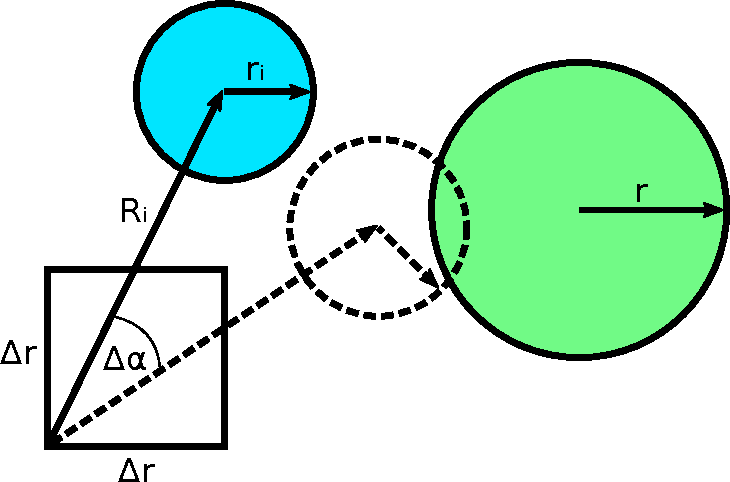
\includegraphics[width=0.7\textwidth,keepaspectratio]{Images/CieslaAlgorithm/drawing.pdf}
	\caption{The green disk is a part of a polydisk already placed within the packing, while the blue disk represents one from a virtual, inserted shape. If at every position and angle within the voxel, the distance between the circle centers is less than the sum of their radiuses, the voxel will be rejected. In this example, the voxel remains active.}
	\label{CieslaAlgorithmDemo}
\end{figure}

\section{Further Development}

The goal of this thesis was to create a GPU-parallel implementation of the algorithm described in this chapter. The algorithm was supposed to generate shapes in the same way as the sequential implementation, but with shorter execution times. \newline
Having the available algorithm for sequential execution, the main challenge consisted of modifying it to enable a highly parallel execution using the GPU. It is described in the following chapter.



\chapter{Proposed Algorithm}

\section {Parallel Application}
The proposed algorithm is expands upon the previously described sequential implementation, in order to utilise the GPU capabilities. It executes some parts sequentially, as it was not possible to parallelise it entirely.

\subsection{Block Diagram}

\begin{figure}[H]
  \centering
	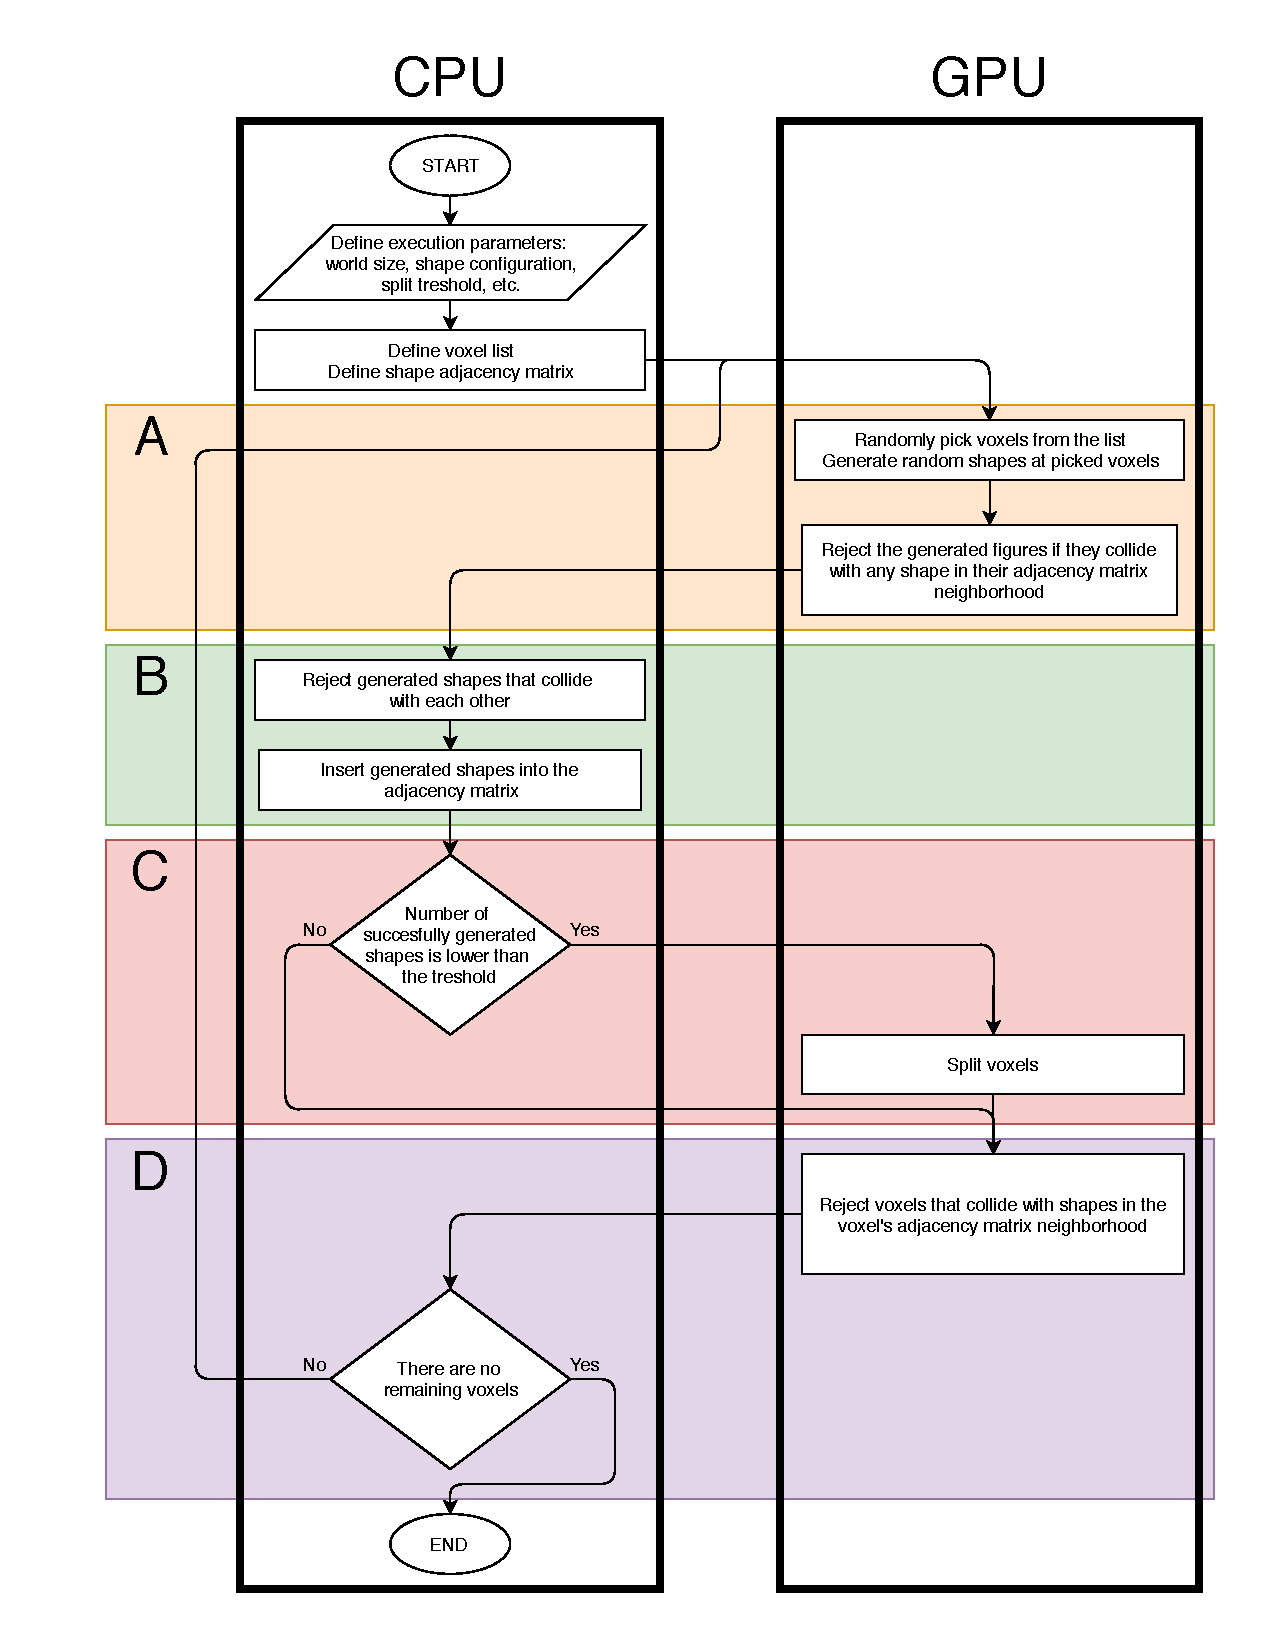
\includegraphics[width=0.9\textwidth,height=0.9\textheight,keepaspectratio]{Images/GPURSA/GPUDiagram1.pdf}
	\caption{This flowchart represents the proposed parallel algorithm. \newline
		Blocks on the right, within the 'GPU' column are executed in parallel, while those on the left are executed sequentially}
	\label{GPURSABlockDiagramPdf}
\end{figure}

\section {Implementation}

The implementation of the algorithm involved several challenges. It necessitated the use of programming tools capable of utilising the GPU processing. Also, a number of smaller auxillary tasks needed to be implemented as well, such as visualisation, optimisation of the shapes, etc.

\subsection{PyCuda}

The Python programming language was chosen to implement these tasks. The ease of writing code, as well as the vast choice of available libraries were deemed crucial in implementing the algorithm. While, as an interpreted language, Python may lack some execution speed, as compared to C or C++, it can partially bridge that gap using the dedicated mathematical libraries such as NumPy. Also, the main acceleration would come from using the parallel approach by utilising the GPU \cite{numpy}. \newline
However, the Python interpreter has no built-in implementation of GPU parallelism, and must rely on external libraries to perform these operations. The library chosen for this task was PyCuda. This library enables the use of Nvidia CUDA's capabilities, simultaneously wrapping parts of it's execution into Python functions. While, it only provides functionalities for initialising the CUDA execution and some basic array operations in Python, it still greately simplifies the code as compared to pure C/C++ implementation. Any more complex parallel code must be written in CUDA C. As such, the code for the algorithm was divided into two parts, where all parallel operations were written in C using CUDA library, while all sequential implementation used Python with PyCuda to initialise and communicate with the GPU-parallel part \cite{pycuda}.


\subsection{Step-by-step Examination}

\subsubsection{Initialisation}

The starting parameters of the algorithm include:
\begin{itemize}
  \item \textbf{The shape configuration} (circle positions and radiuses relative to the shape origin).
  \item \textbf{Number of added shapes} per iteration.
  \item Adjacency matrix \textbf{cell size} (must be greater than the shape size).
  \item \textbf{World size} (in number of adjacency matrix cells).
	\item \textbf{Voxel split treshold} - the proportion of added shapes that were rejected that would trigger the voxel split.
\end{itemize}
As these parameters are set, a number of additional functions are executed. The shape area is being calculated, and the shape itself is being optimised. The latter involves re-calculating the origin of the shape, so that it's bounding circle is the smallest. These functions are auxillary to the main algorithm.
\newline
During the initialisation, there are created the data structures used throught the further execution. These involve:
\begin{itemize}
  \item \textbf{The shape array}: An array with shape: $3 \times N$, where N is the number of shapes in the packing. Every row has the shape's coordinates (x,y) and it's angle.
  \item \textbf{The neighborhood matrix}: The 3D array with shape: $CX \times CY \times SPN$ where CX and CY are the world dimensions in numbers of cells, while SPN is the theoretical maximum of shapes per $3 \times 3$ cells (overestimated approximate). Such groupings of cells are here referred to as the "neighborhoods", and they contain the indexes of shapes that may collide with a shape in a given adjacency matrix cell. This data structure serves as the adjacency matrix.
  \item \textbf{The voxel array}: Similar to the shape array, it contains the spatial and angular positions of the existing voxels.
\end{itemize}
Additionally, there are set variables that are subject to change: the \textbf{current voxel spatial size} and the \textbf{current voxel angular size}. Initially, the voxels are cell-sized, with the angular size of $2 \pi$
Finally, the CUDA parallel execution is initialised, and it's pseudorandom generator is seeded with the current time.

\subsubsection{Part A: Shape generation}

\begin{figure}[H]
  \centering
	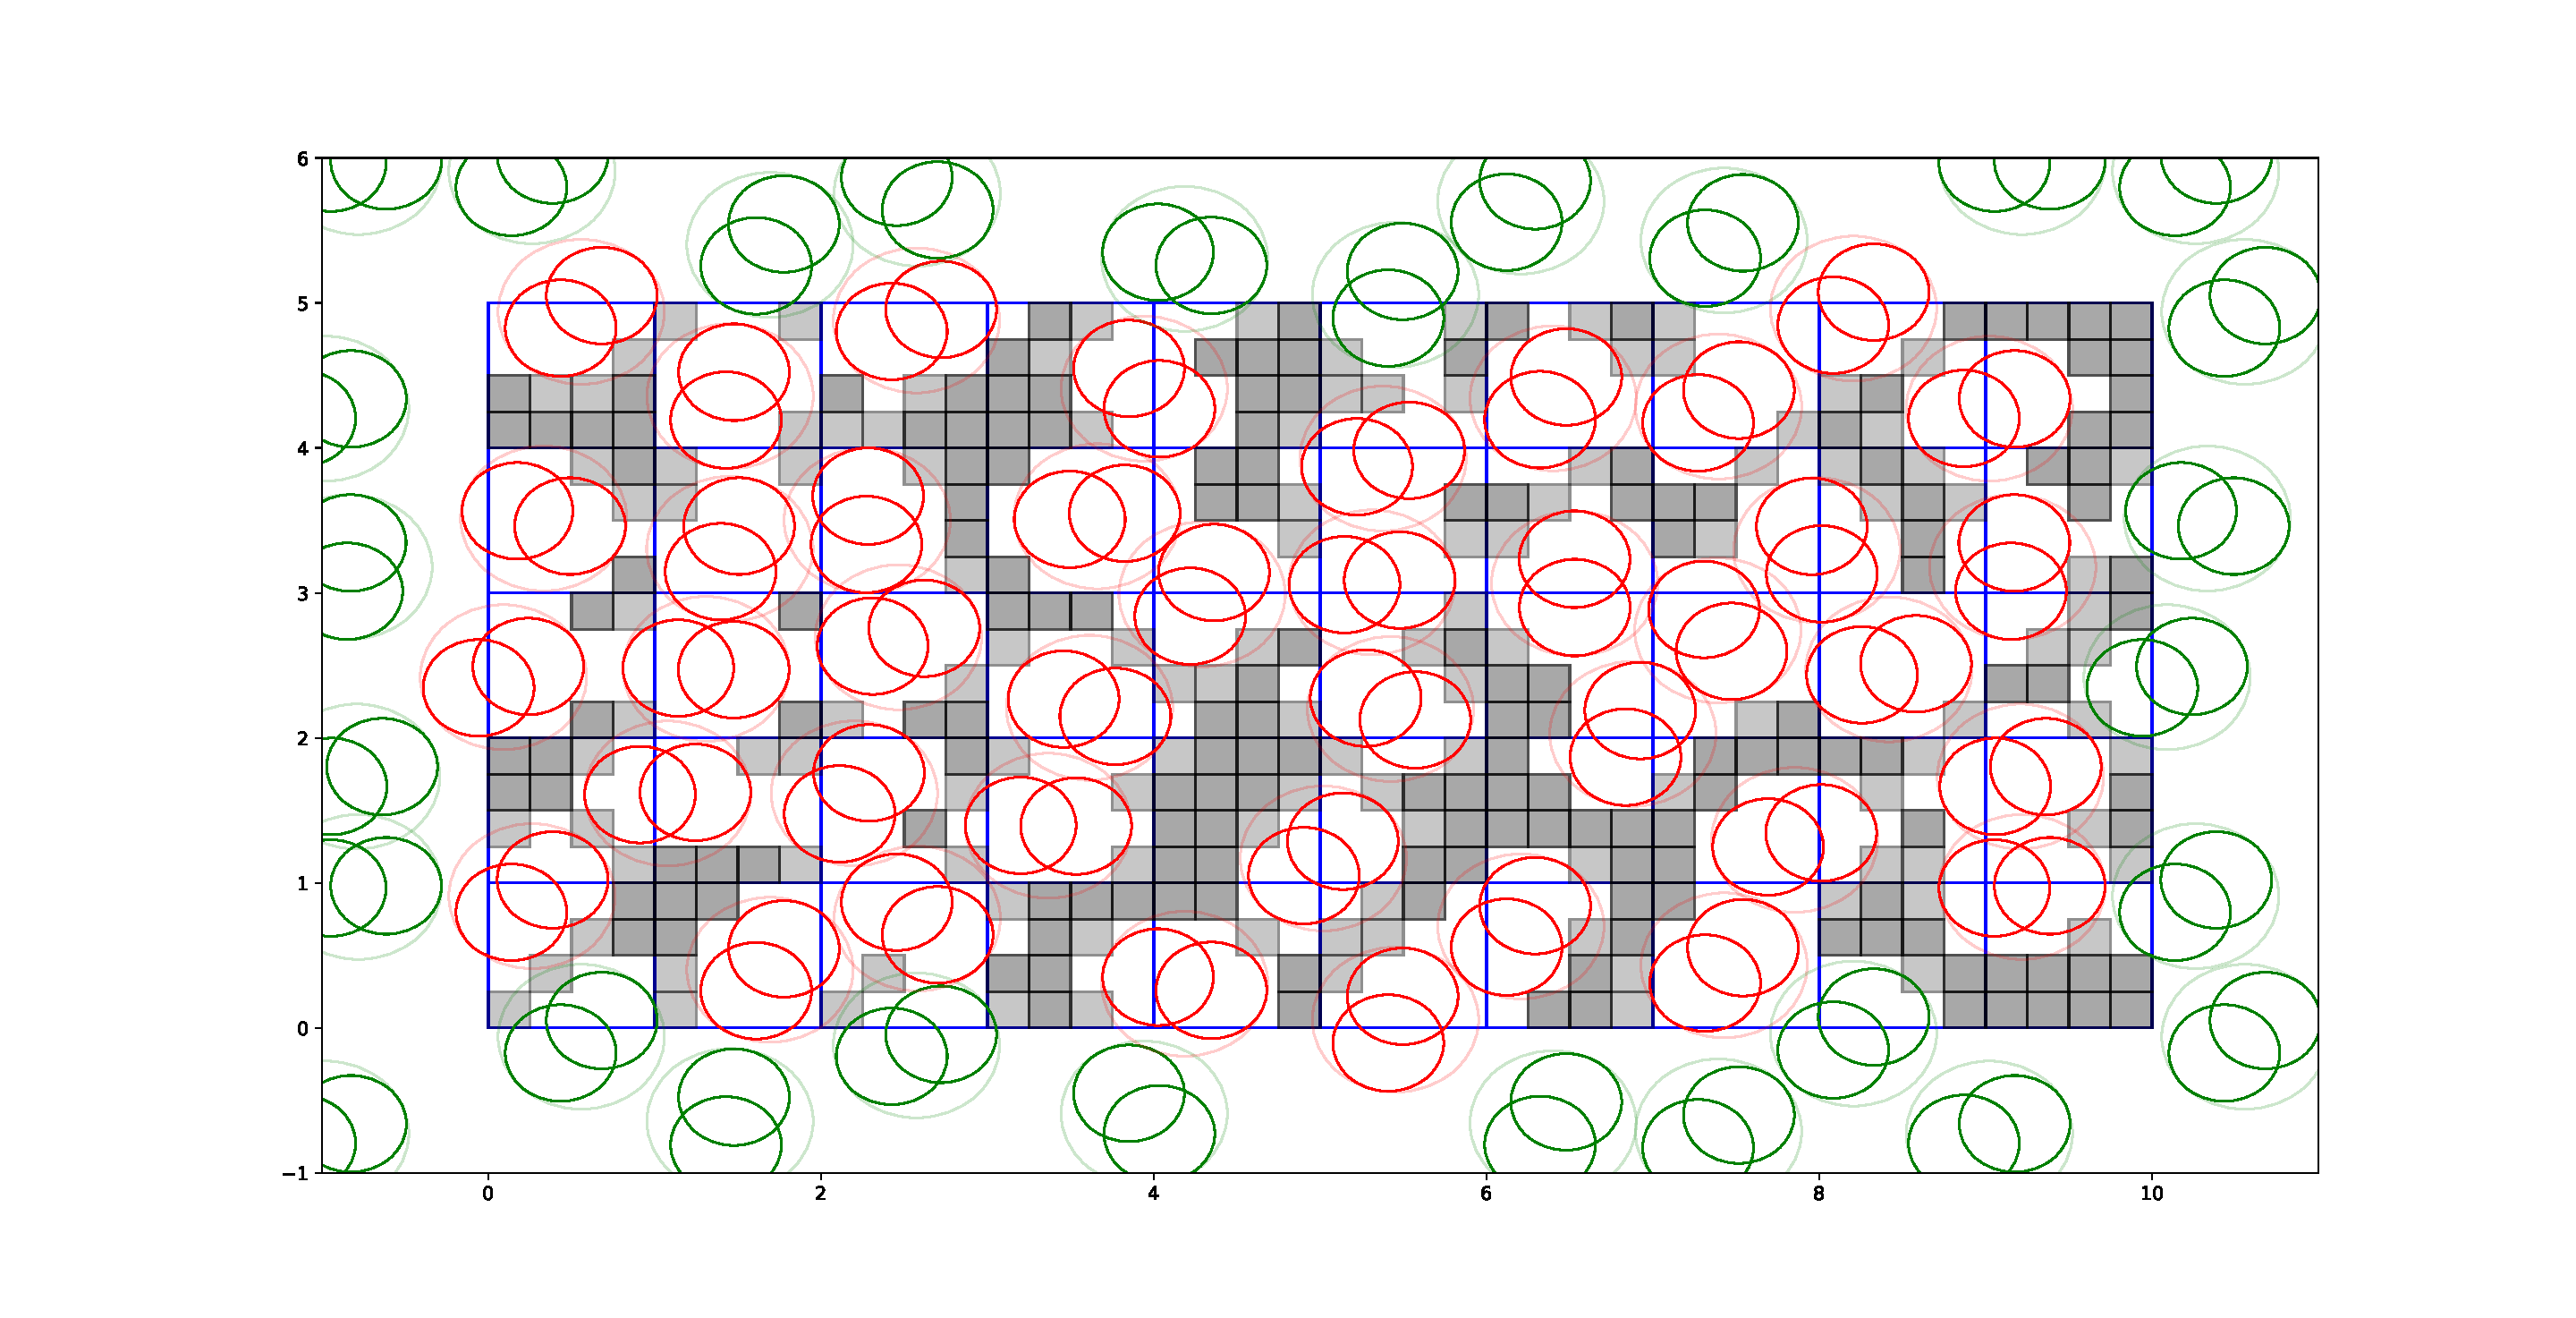
\includegraphics[width=0.9\textwidth,keepaspectratio]{Images/GPURSA/Figure_1.pdf}
	\caption{The packing after several iterations, before generating a new set of shapes.\newline
	The existing shapes are marked in red. The shapes appearing at the edges, as a part of periodic boundary conditons are green. The faint circles around the shapes are their bounding circles. The empty, blue squares represnt the cells of the adjacency matrix. The gray, partially translucent squares represent the voxels. The darker squares represent multiple voxels with different angle ranges occupying the same coordinates.}
	\label{GPURSA_Process_1}
\end{figure}

%MAY BE GOTTEN RID OF START
\begin{figure}[H]
  \centering
	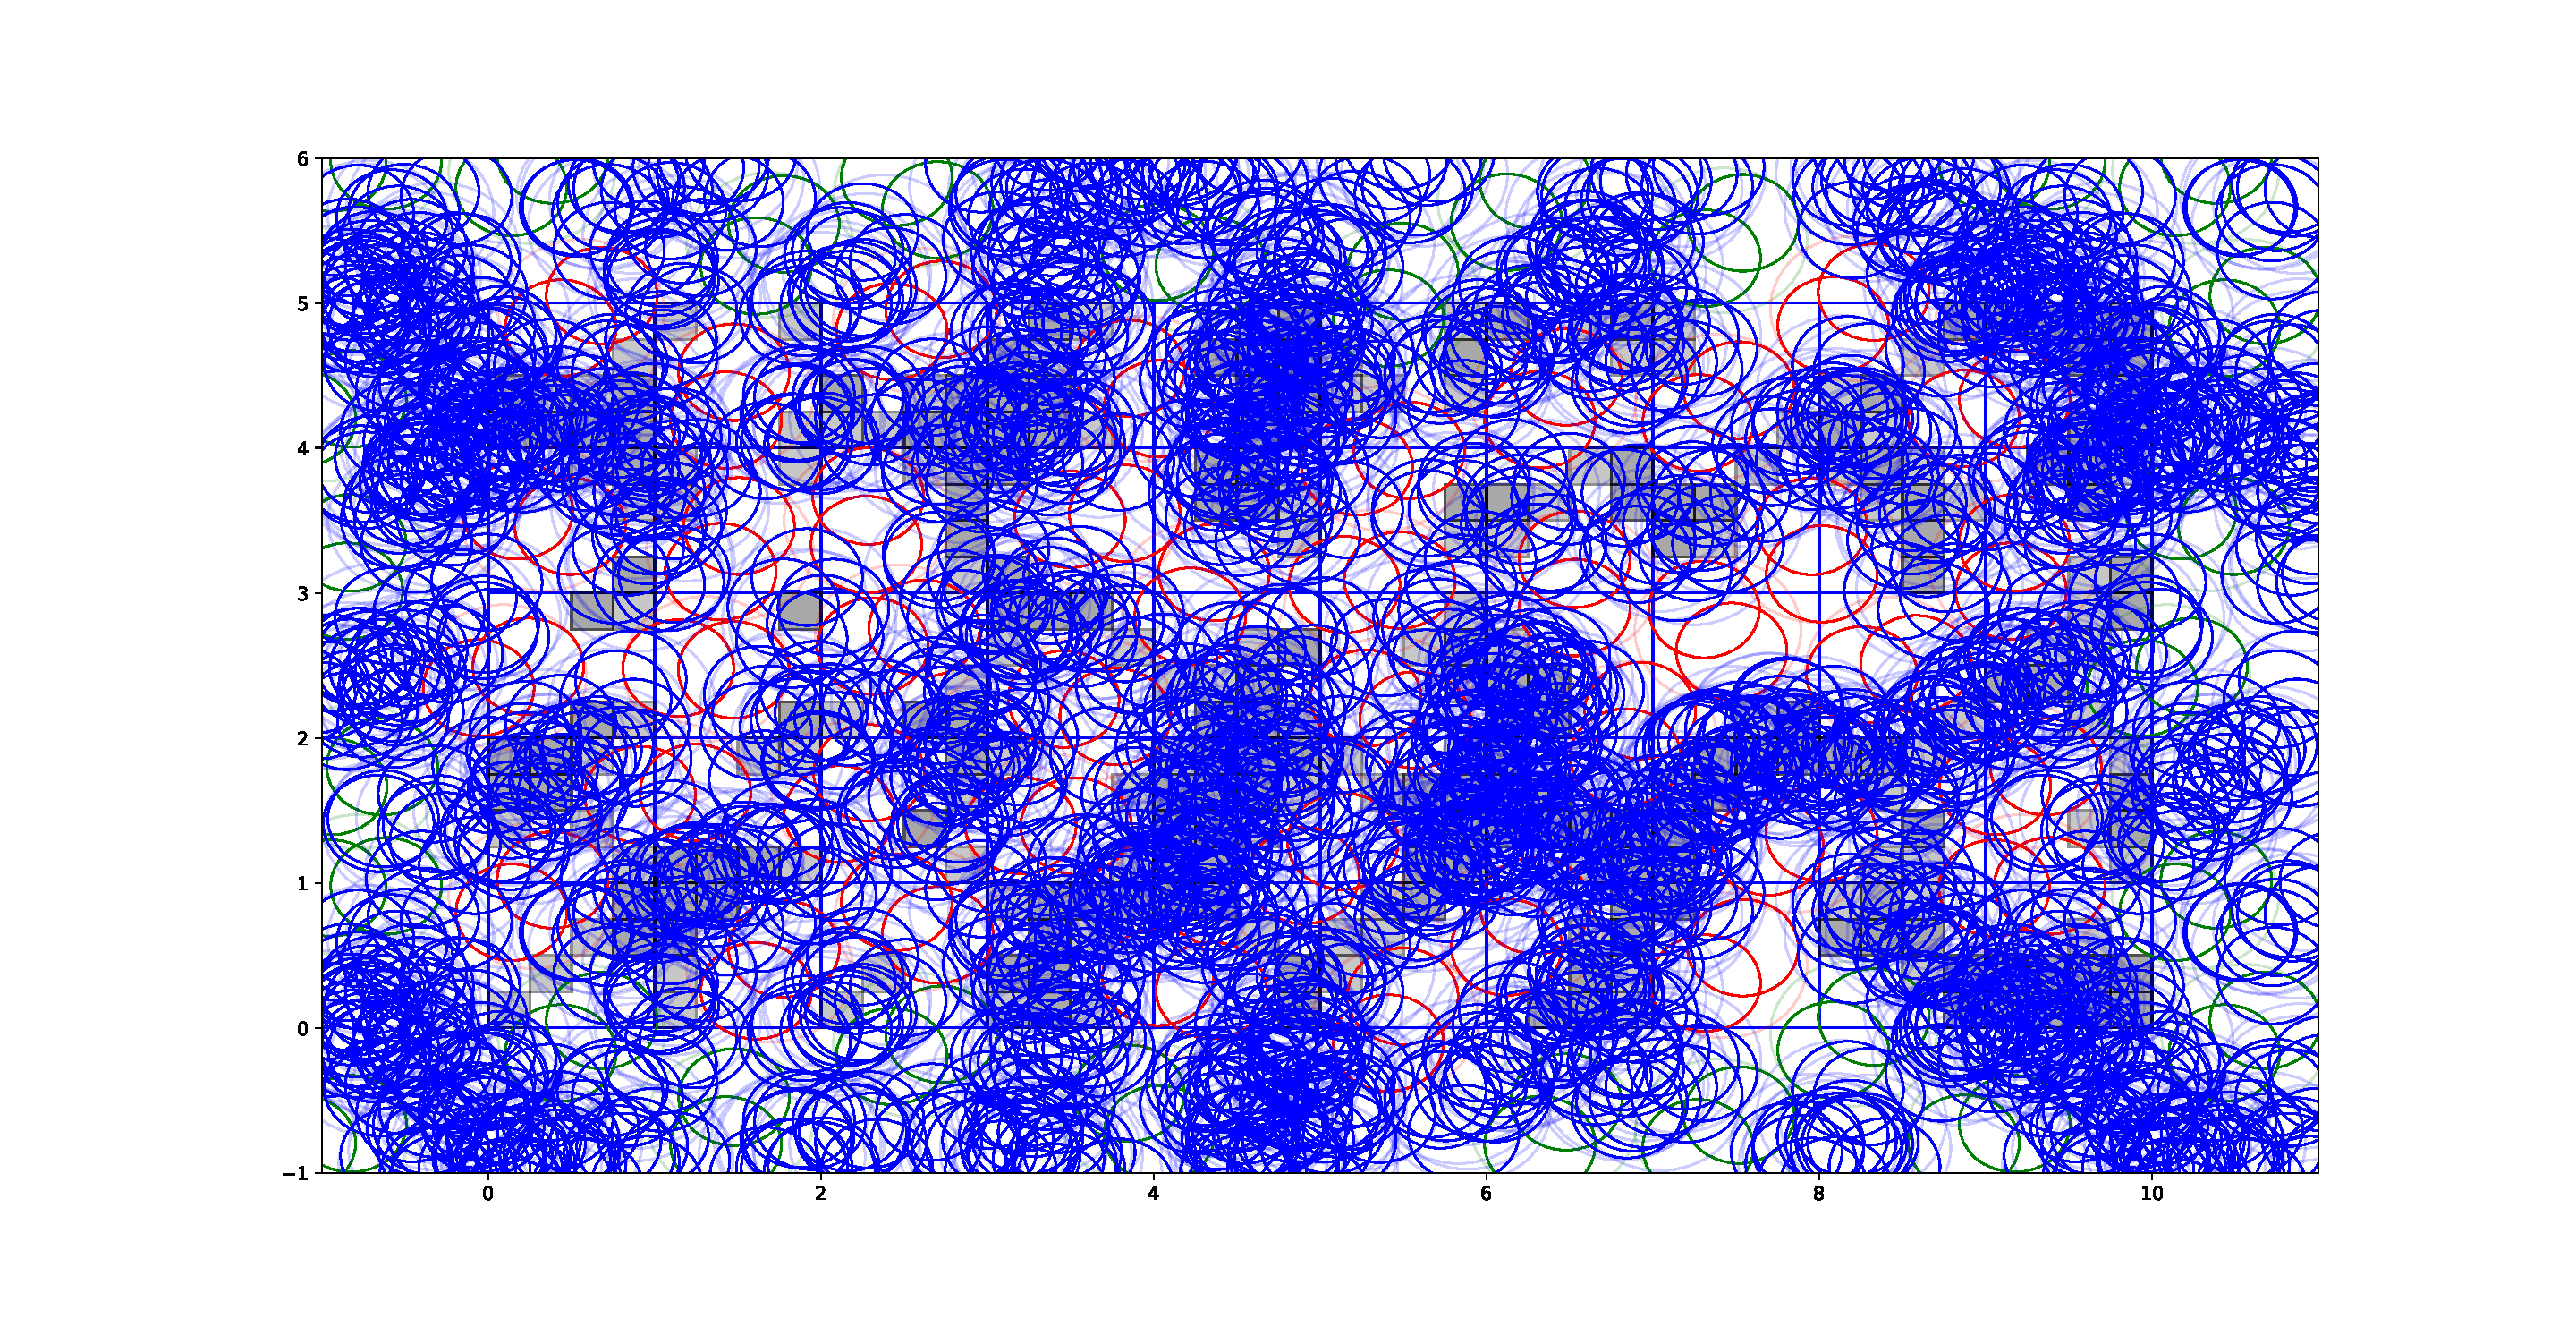
\includegraphics[width=0.9\textwidth,keepaspectratio]{Images/GPURSA/Figure_2.pdf}
	\caption{The packing after shape generation. The mass of new shapes (blue) cluttering the packing was generated randomly at existing voxels.}
	\label{GPURSA_Process_1}
\end{figure}
%MAY BE GOTTEN RID OF END

This part is executed entirely in parallel. \newline
In this part, an additional array, \textbf{the added shape array} is created. It will be later merged with \textbf{the shape array}. \newline
A number of CUDA threads is created, equal to \textbf{the number of added shapes}. Every thread randomly picks a voxel from the \textbf{the voxel array}. A shape is generated with it's poisition and angle within the voxel. The resulting shapes are put into the \textbf{the added shape array}.

\subsubsection{Part B: Shape rejection against pre-existing shapes}

\begin{figure}[H]
  \centering
	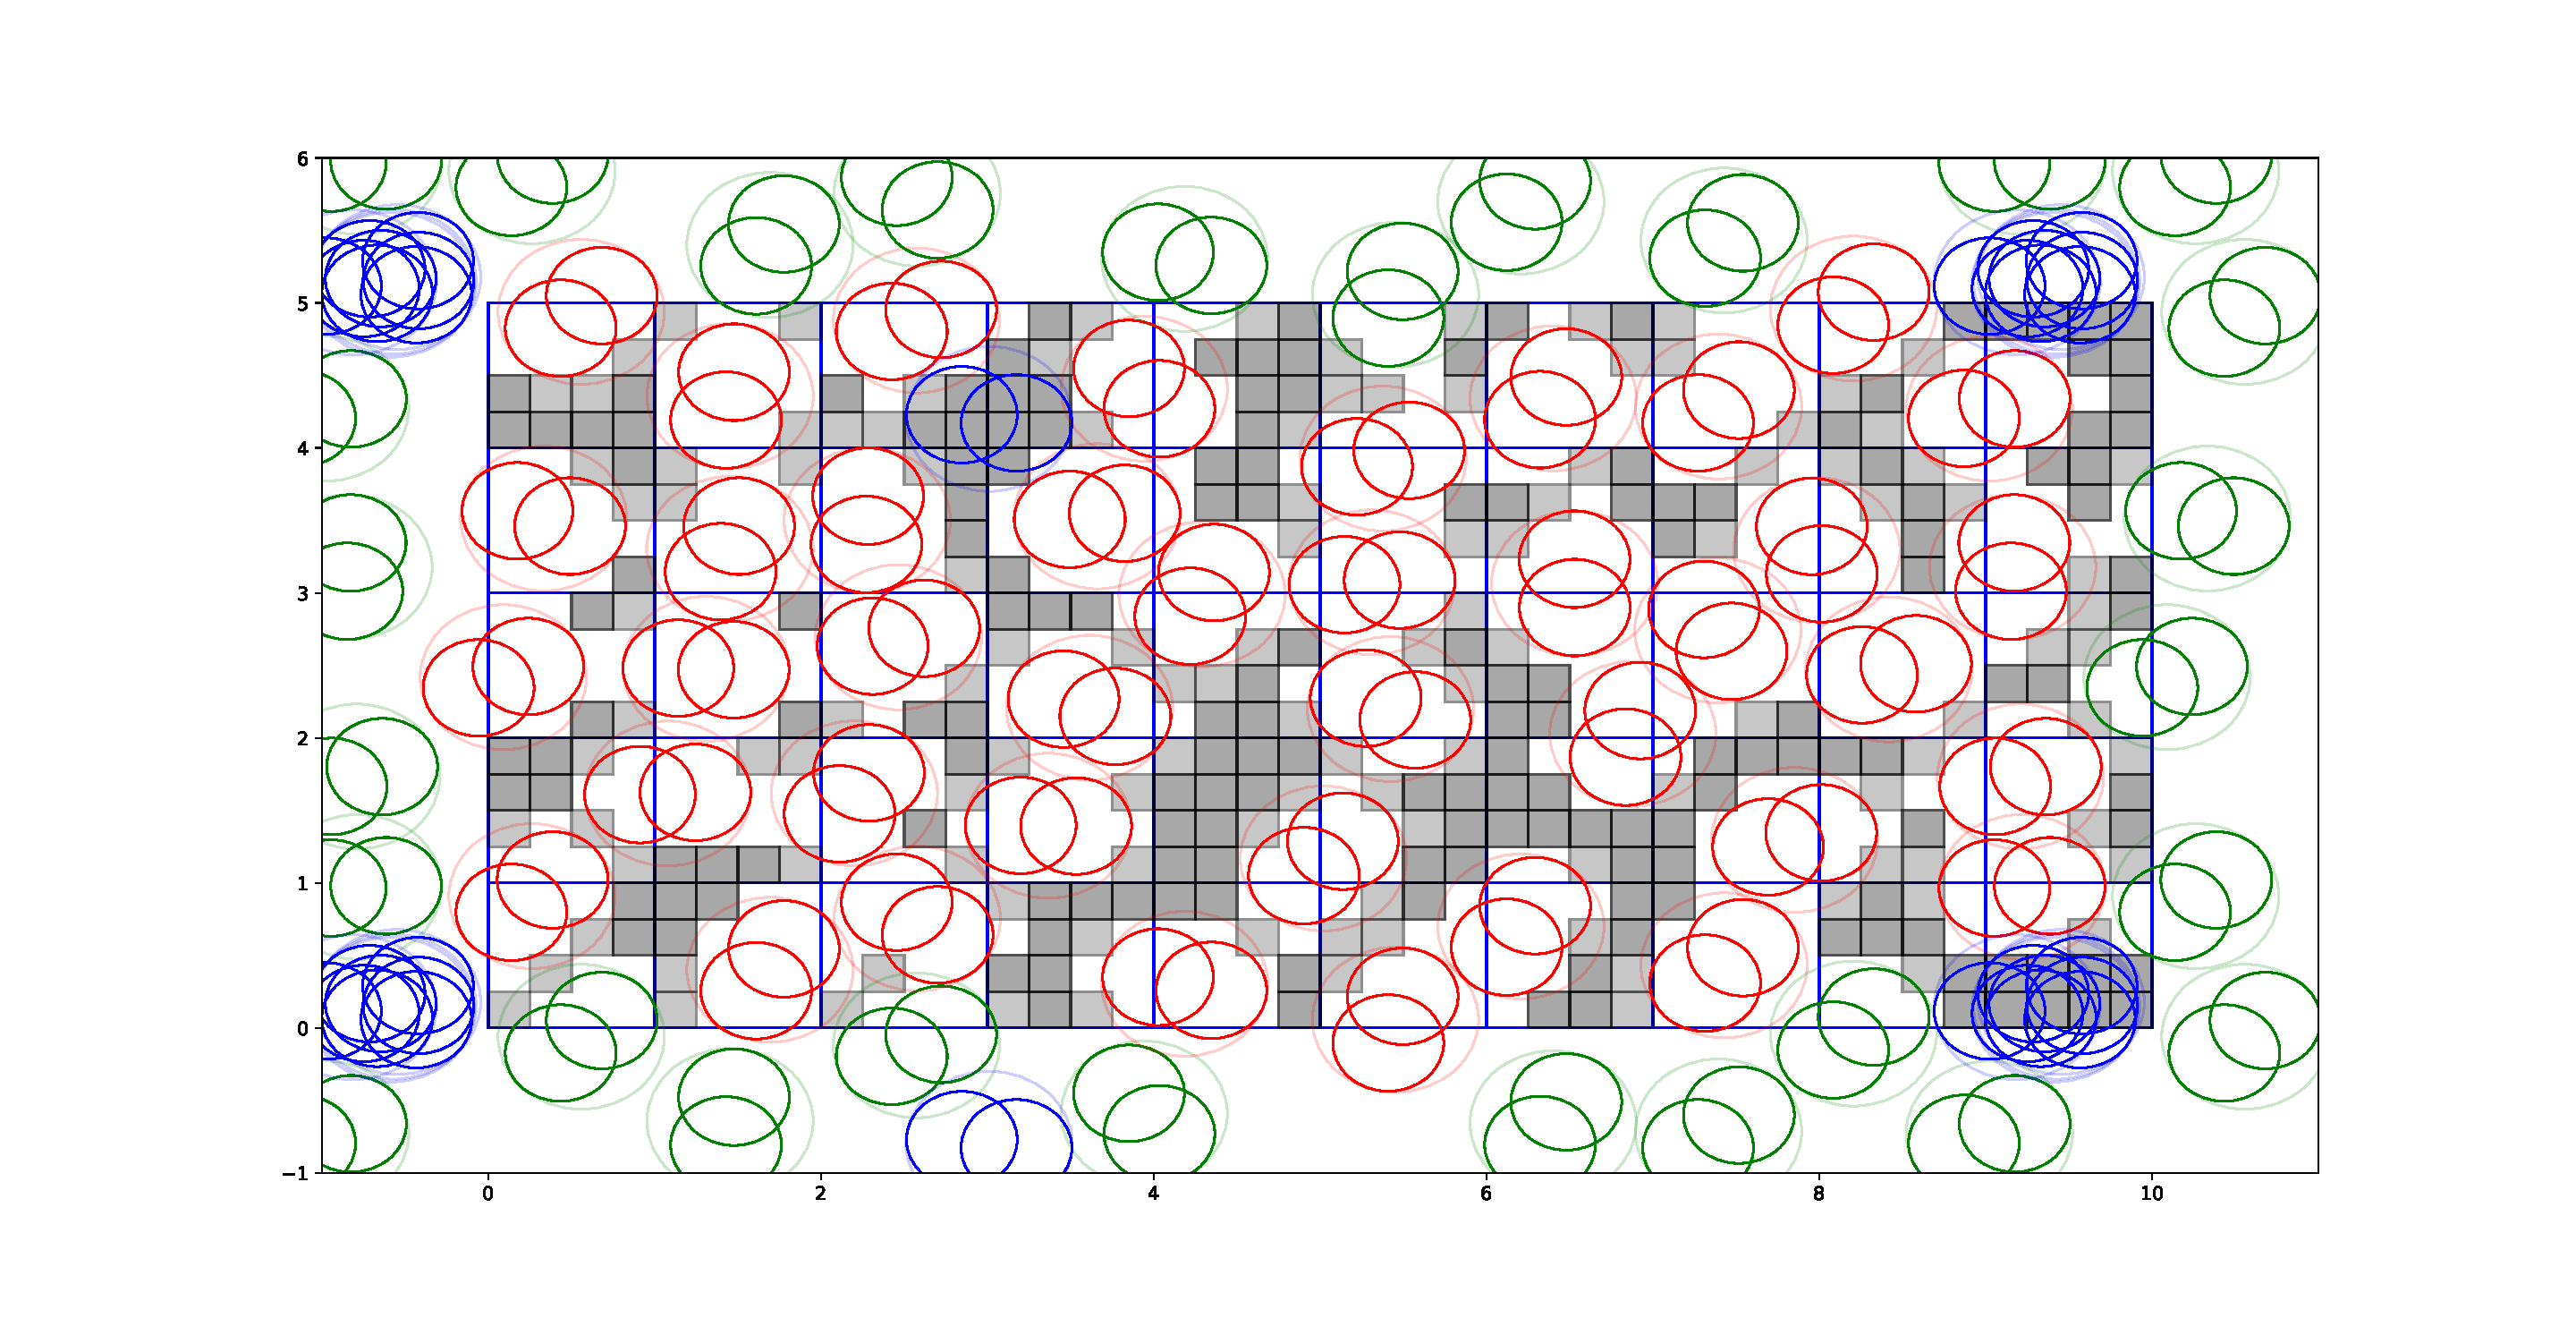
\includegraphics[width=0.9\textwidth,keepaspectratio]{Images/GPURSA/Figure_3.pdf}
	\caption{Packing after rejection of shapes against the pre-existing ones. Only small groupings of new shapes remain. The pre-existing shapes are red and green, in the same way as in figure \ref{GPURSA_Process_1}. The new polydisks are blue, including those appearing due to periodic boundary conditions}
	\label{GPURSA_Process_2}
\end{figure}

This part is executed entirely in parallel. \newline
The same GPU threads are used as in the last part, each corresponding to a generated shape. The shapes' adjacency matrix cell positions are calculated. Basing on this, the collision is detected between the shape in the thread and all of the already existing shapes in it's potential neighborhood. If the shape collides with any of the pre-existing shapes, it is rejected, which is marked by setting it's coordinates in \textbf{the added shape array} to [-1.0,-1.0,-1.0]

\subsubsection{Part C: Shape rejection against other new shapes}

\begin{figure}[H]
  \centering
	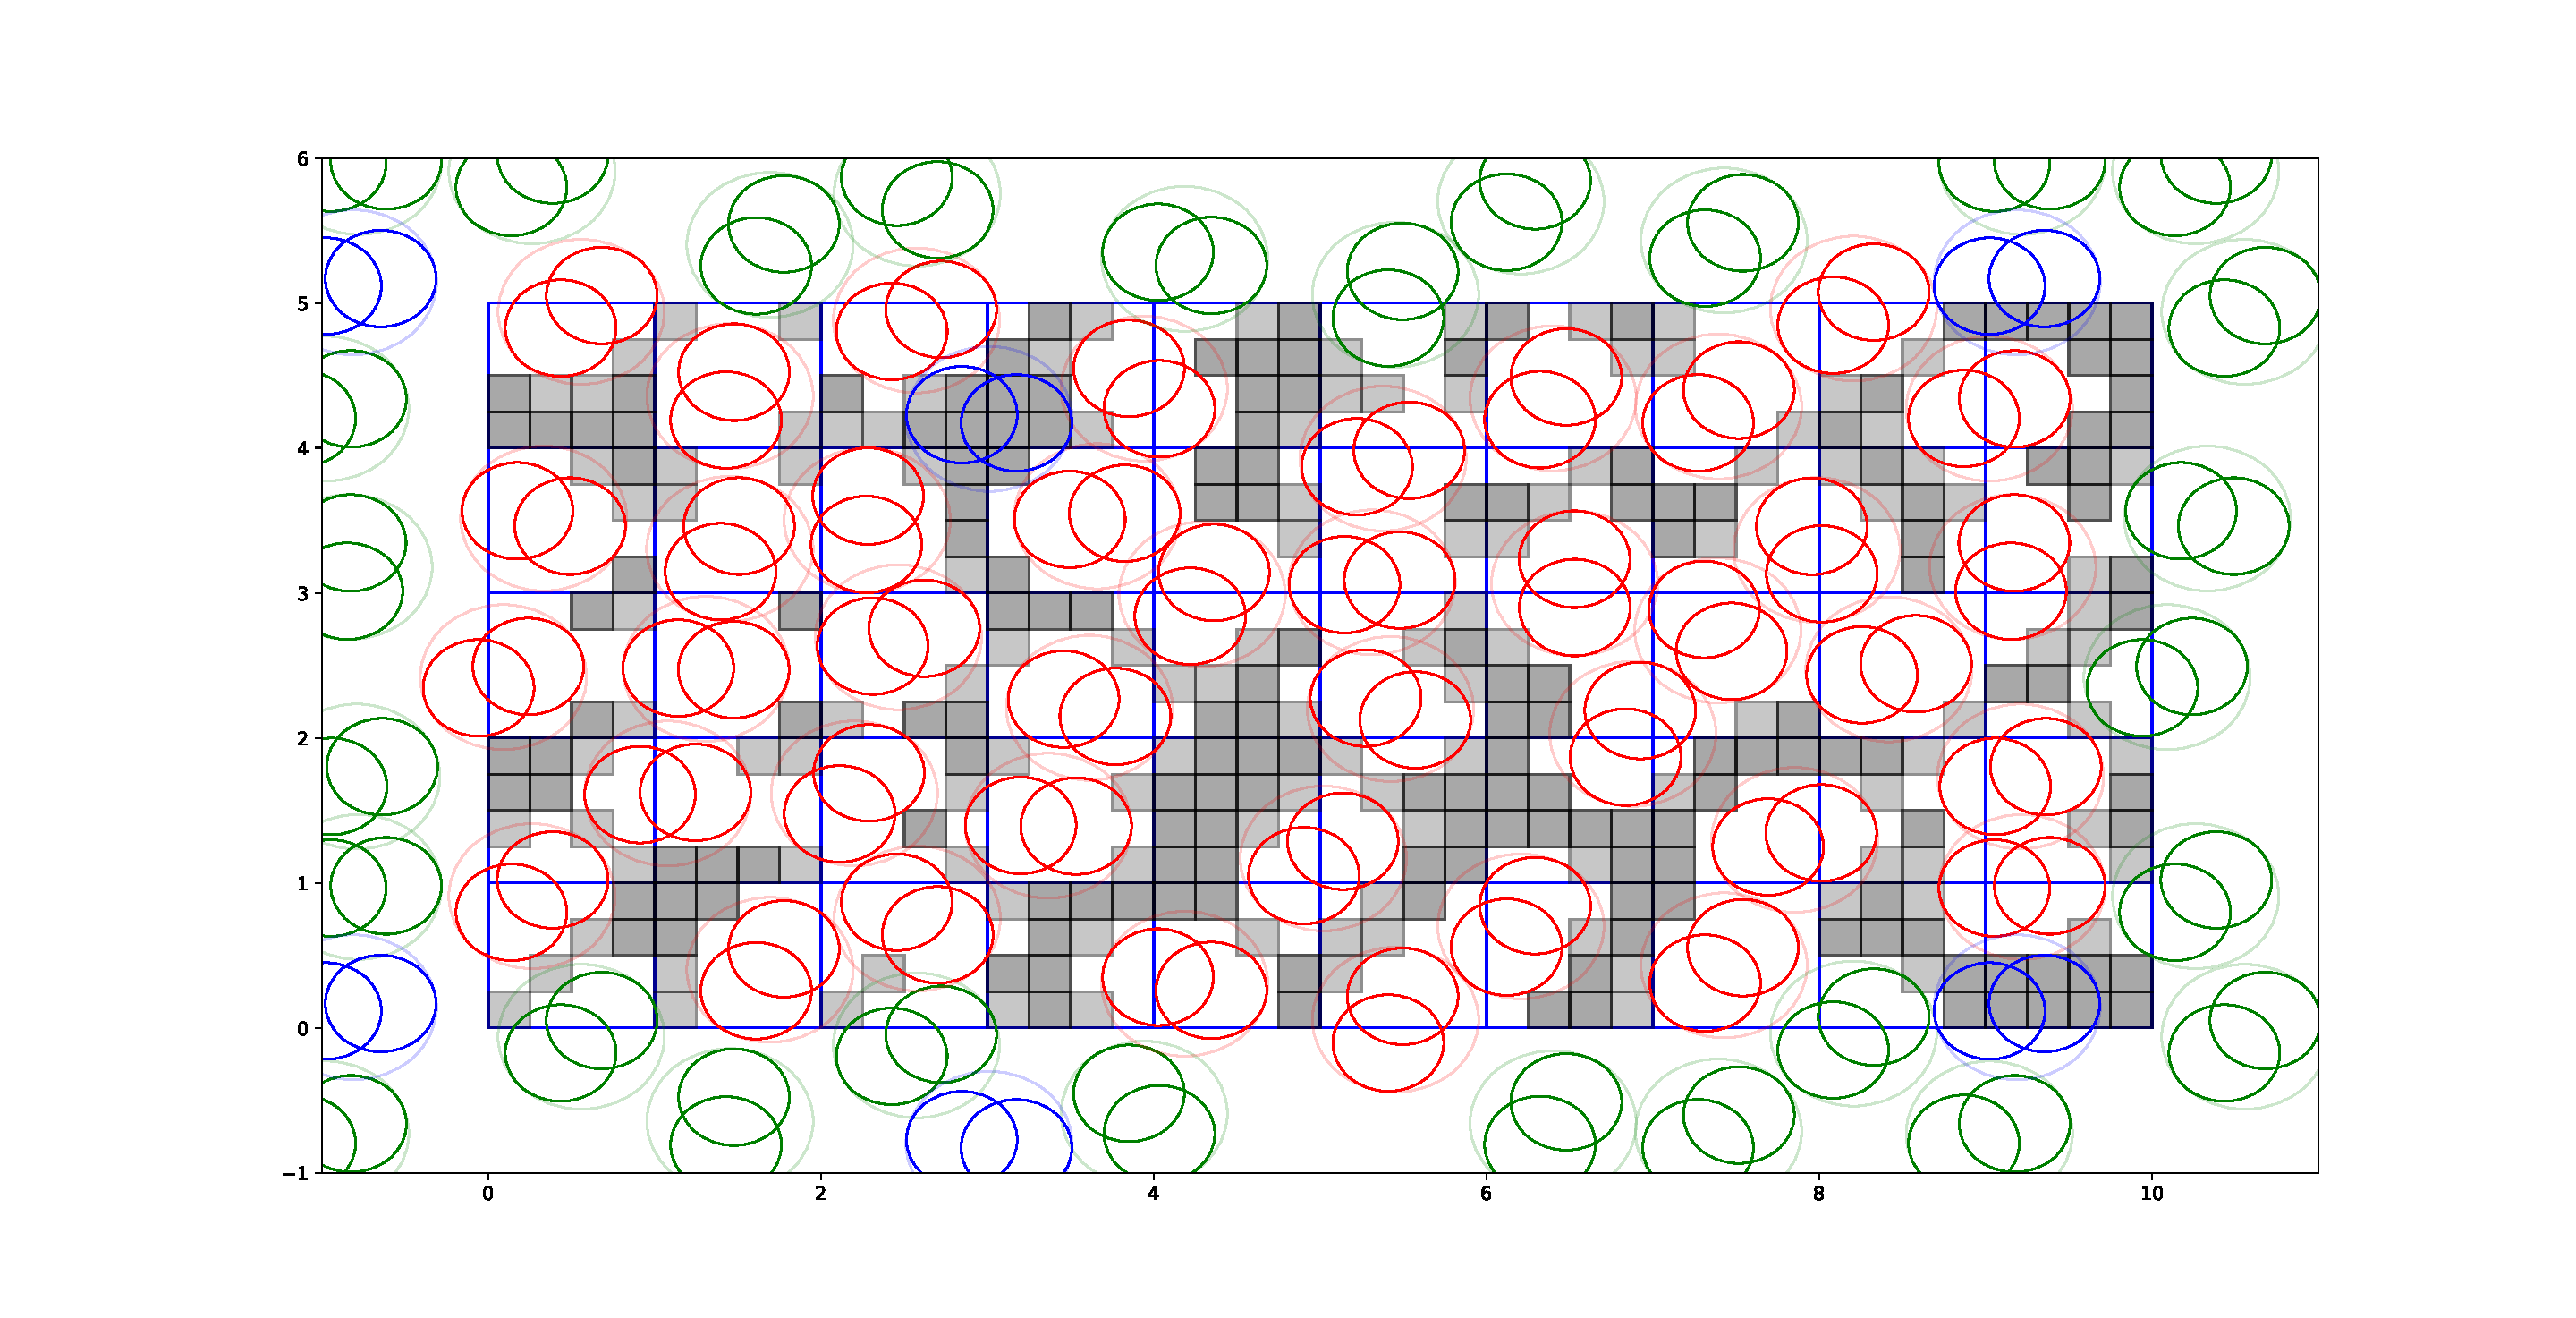
\includegraphics[width=0.9\textwidth,keepaspectratio]{Images/GPURSA/Figure_4.pdf}
	\caption{Packing after rejecting the remaining new shapes against each other.}
	\label{GPURSA_Process_4}
\end{figure}

This part is executed sequentially. \newline
\textbf{The added shape array} is returned from the CUDA execution, and "squashed" to remove all rejected shapes. Since the shapes do not collide against any pre-existing ones, only the collisions within the list of new shapes need to be calculated. A temporary, empty neighborhood matrix is created. Shapes are added to this matrix sequentially, and rejected if they collide with one existing there. When all shapes are added, the shapes are merged into the actual \textbf{neighborhood matrix}, and \textbf{the added shape array} is concatentated to \textbf{the shape array}.

\subsubsection{Part D: Voxel splitting}

\begin{figure}[H]
  \centering
	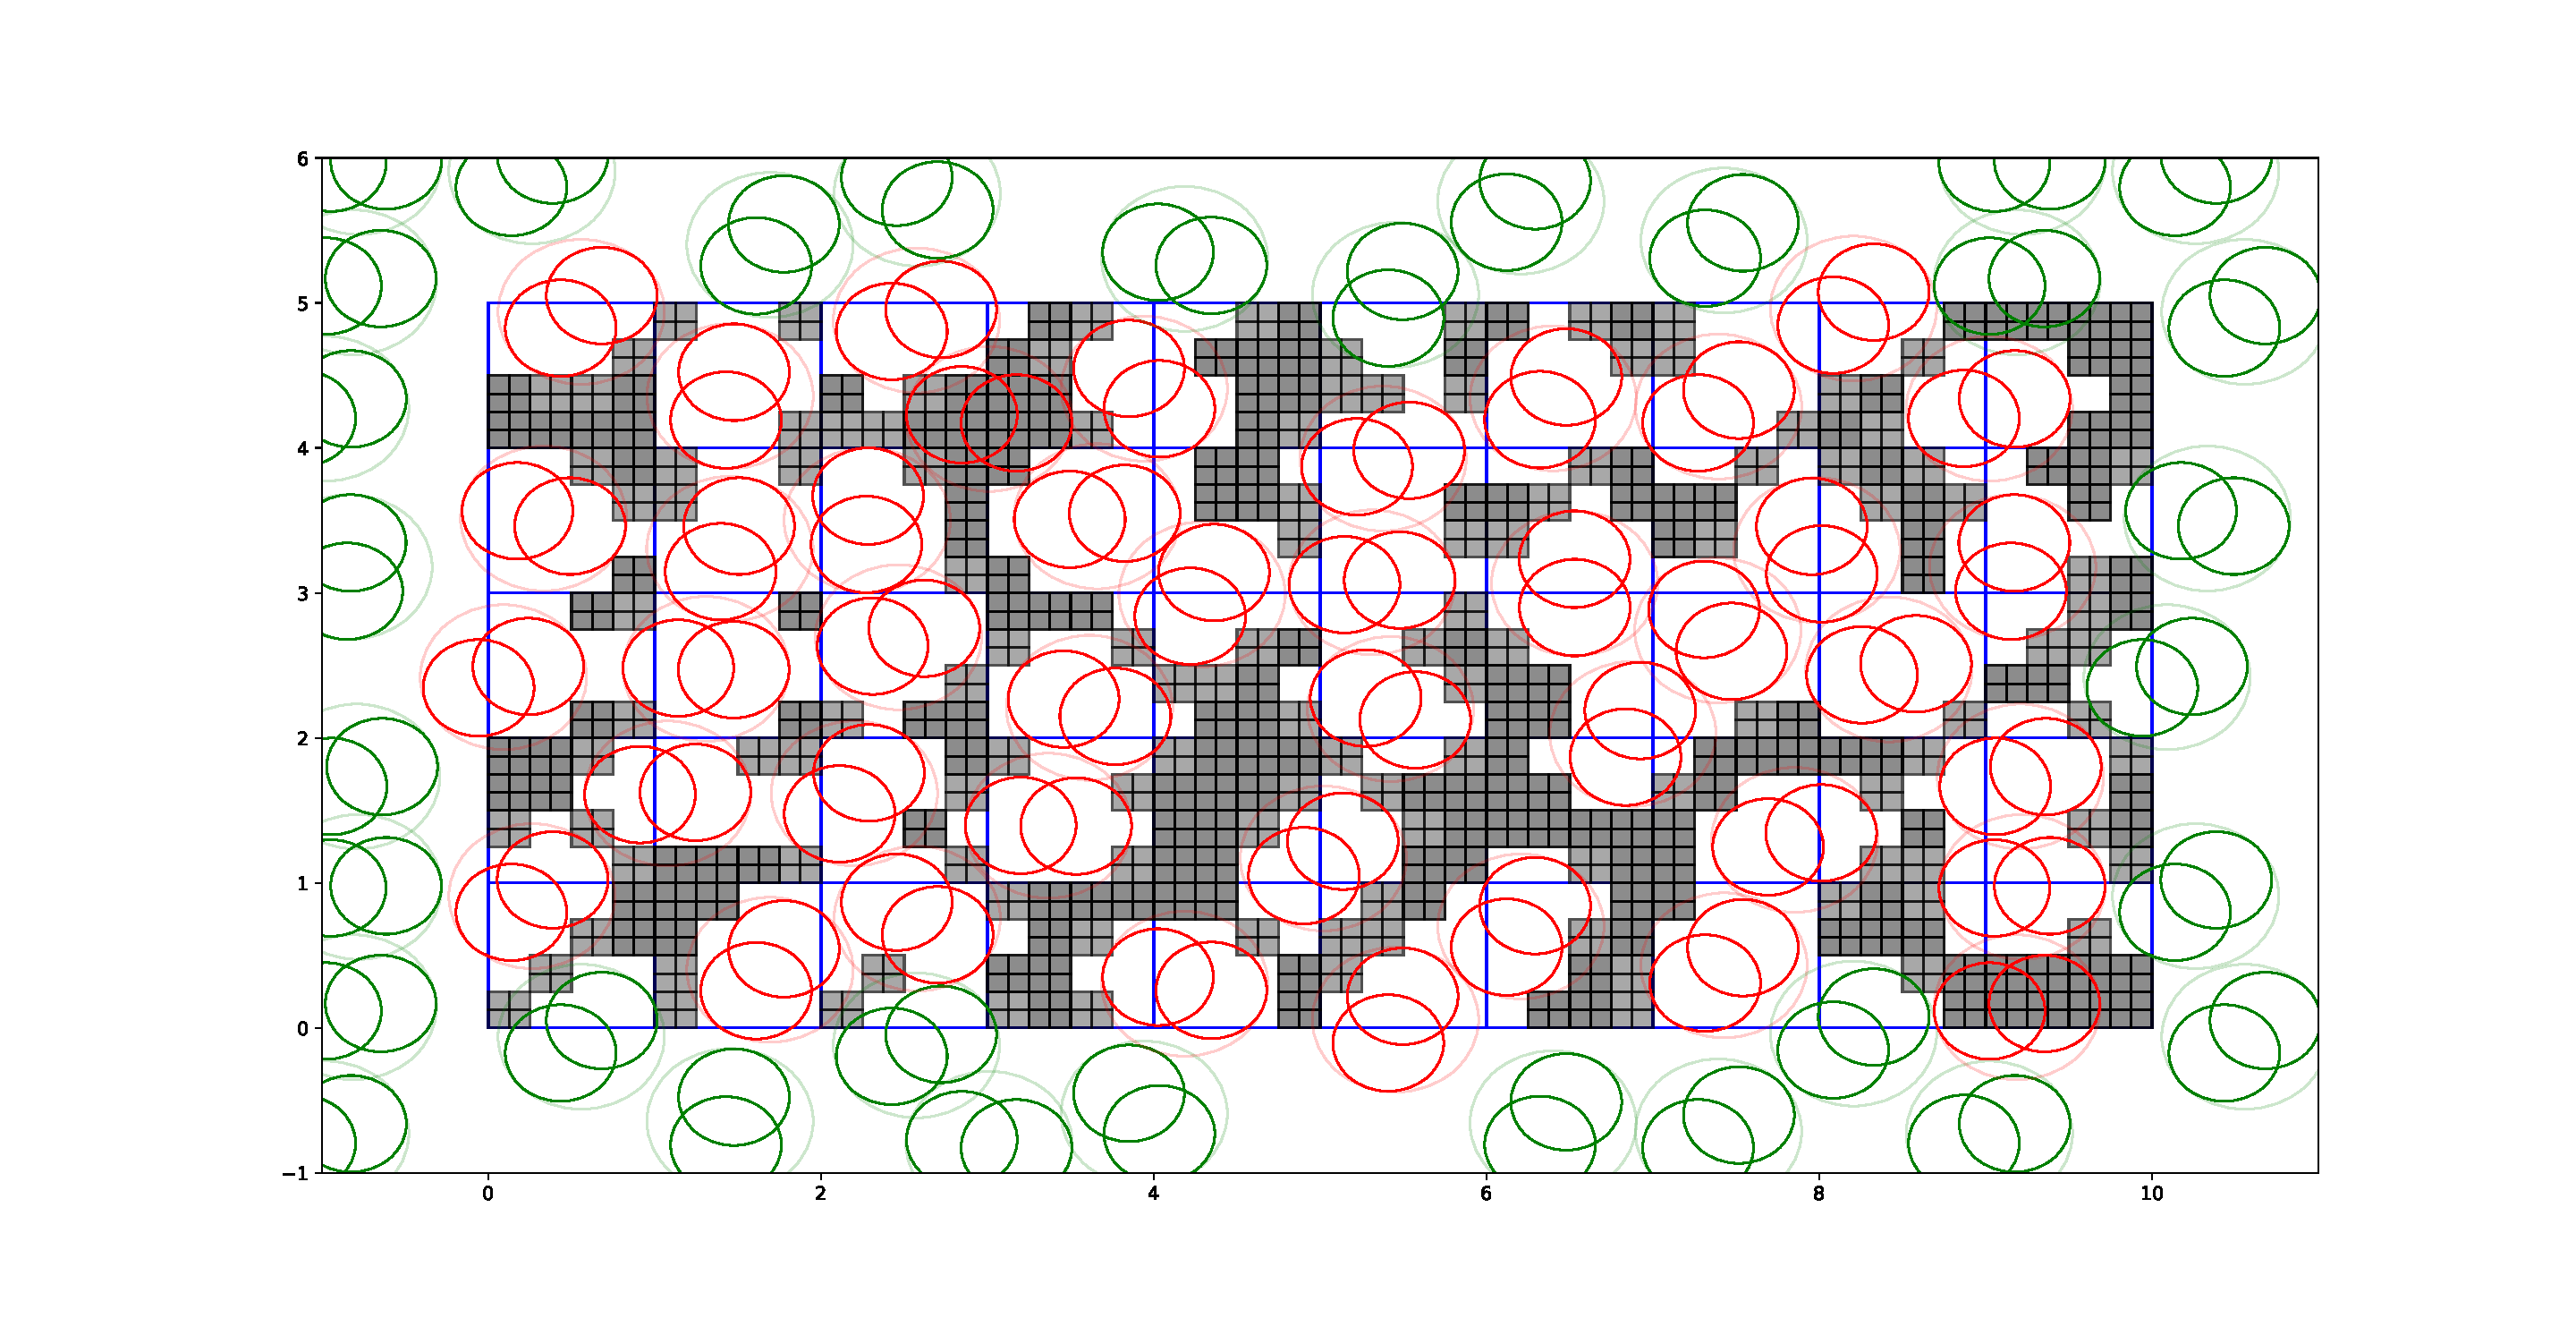
\includegraphics[width=0.9\textwidth,keepaspectratio]{Images/GPURSA/Figure_5.pdf}
	\caption{Packing after voxel splitting. Every old voxel has been split into eight new ones.}
	\label{GPURSA_Process_5}
\end{figure}

This part is executed entirely in parallel. \newline
If the proportion of shapes succesfully added to the packing in the previous part is lower than \textbf{the voxel split treshold}, this part is executed. \newline
The number of CUDA threads is created, for every currently existing voxel. A temporary new array, \textbf{the new voxel array} is created, with eight times as many elements as \textbf{the voxel array}. In every thread, the voxel is being split into 8 new ones, each with halved dimensions, and given new positions, so that they cover the entirety of their "predecessor". These voxels are placed in \textbf{the new voxel array} which afterwards replaces \textbf{the voxel array}.
The values of \textbf{the voxel spatial size} and \textbf{the voxel angular size} are halved.

\subsubsection{Part E: Voxel rejection}

\begin{figure}[H]
  \centering
	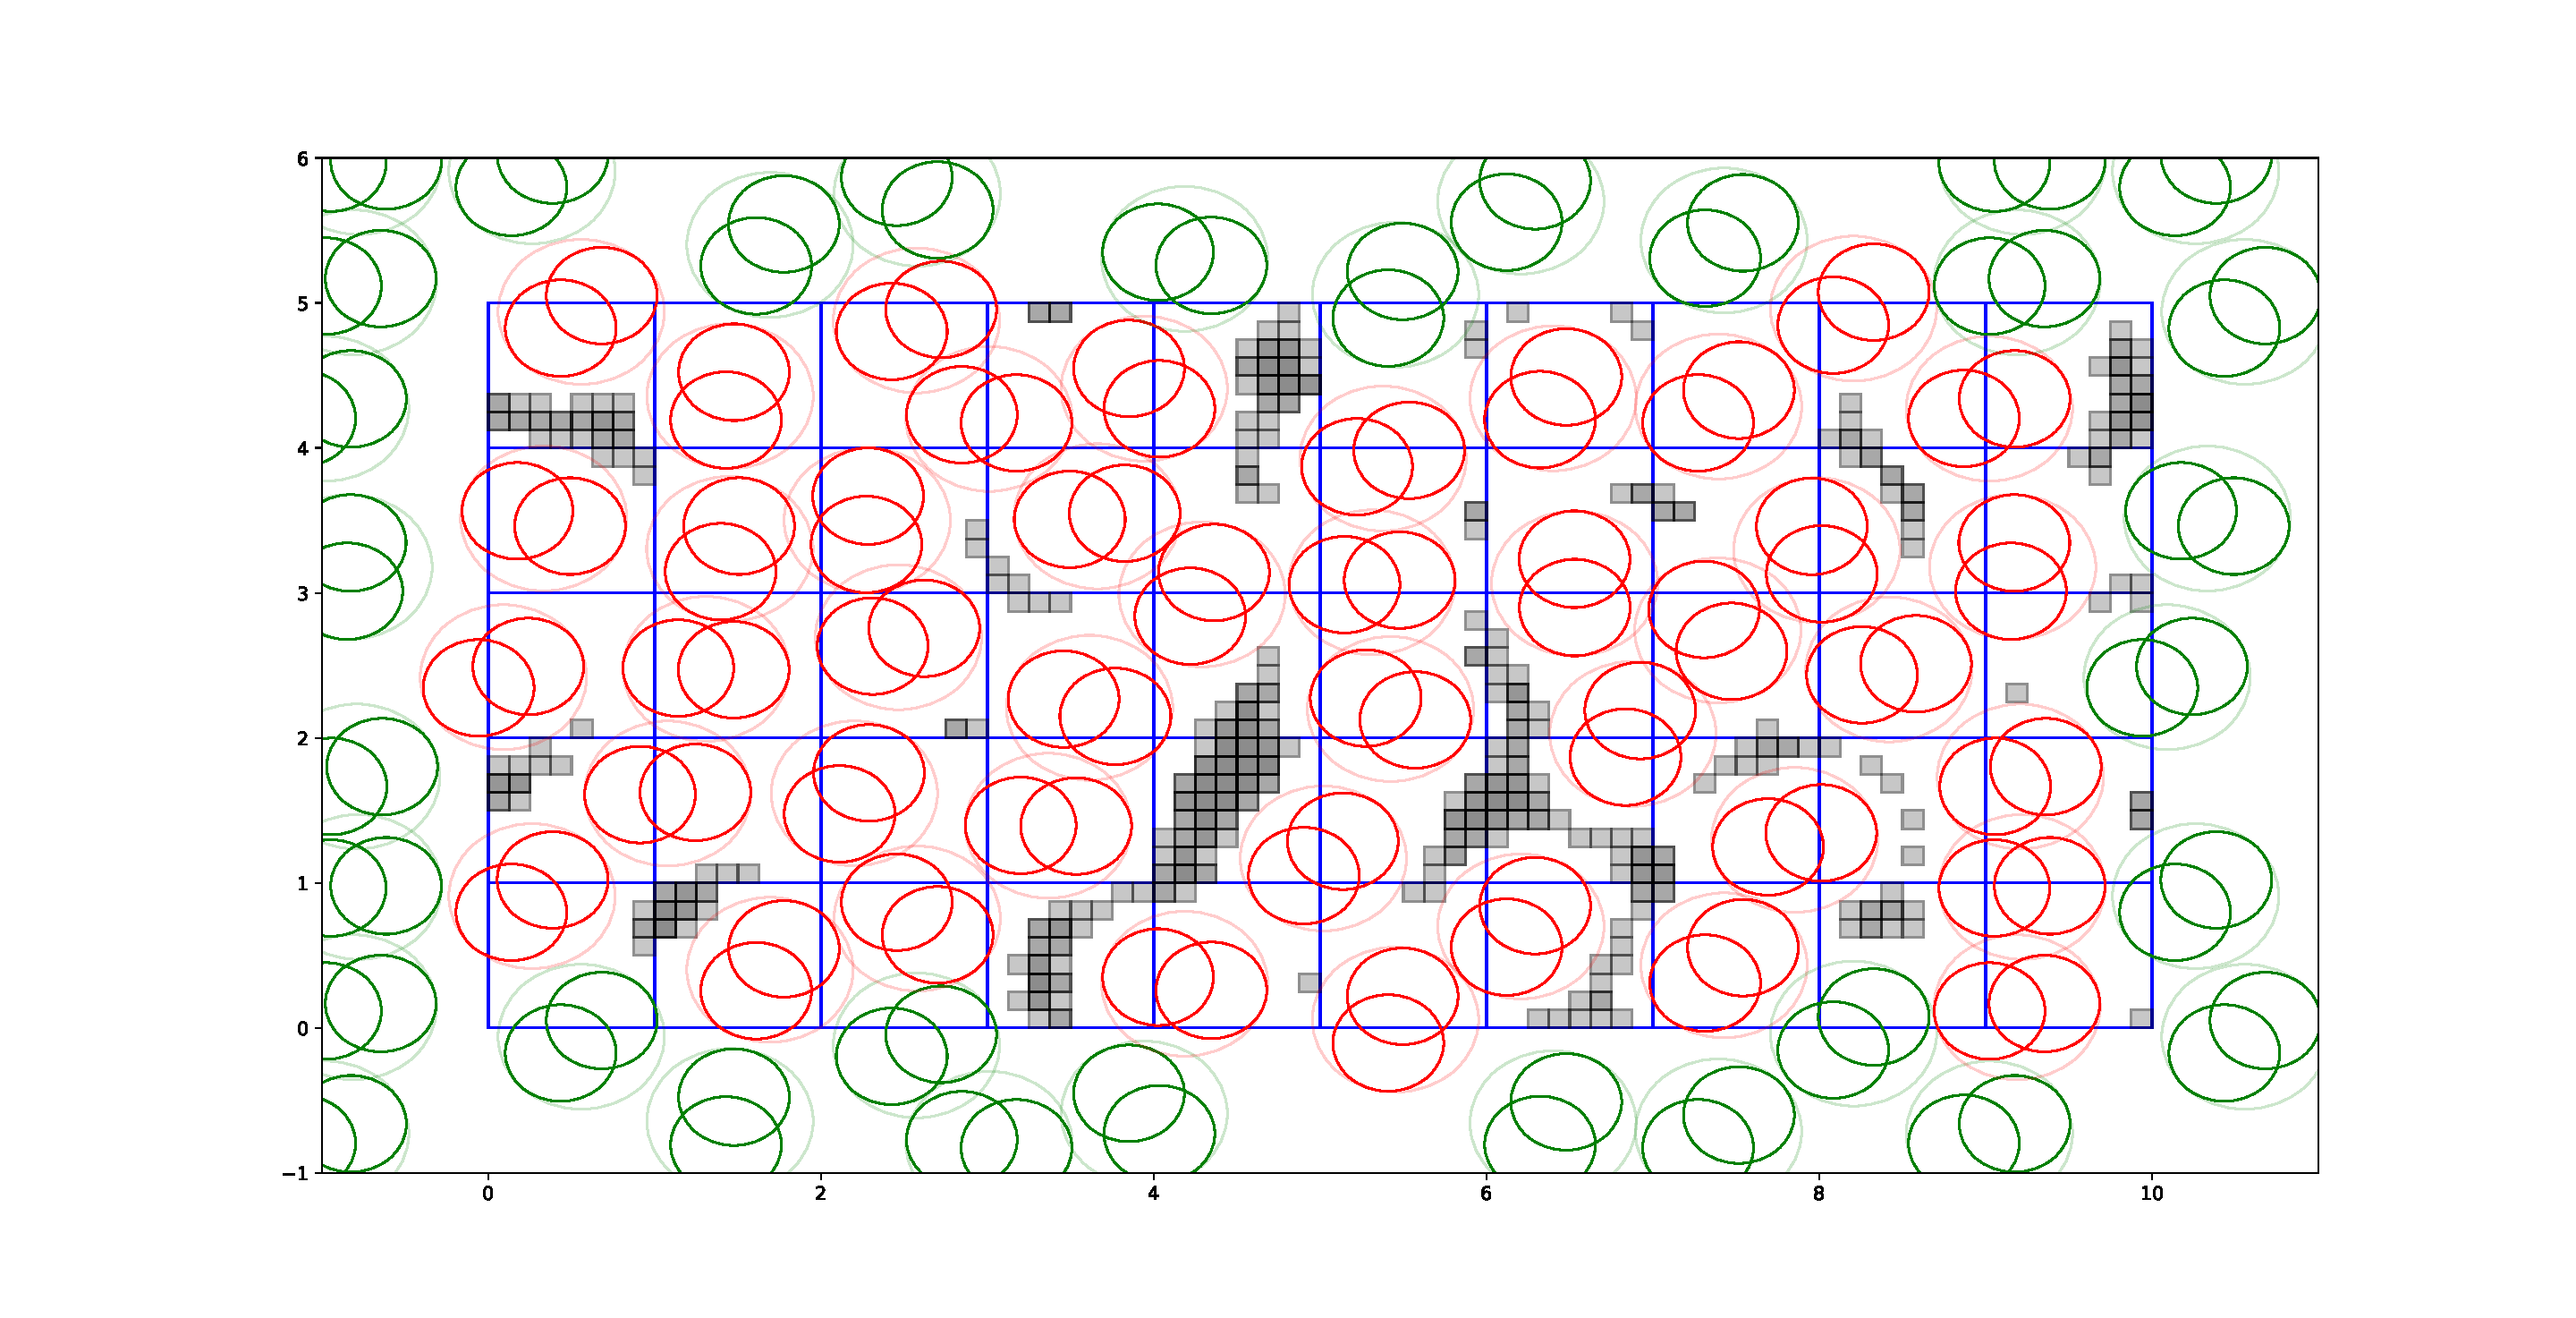
\includegraphics[width=0.9\textwidth,keepaspectratio]{Images/GPURSA/Figure_6.pdf}
	\caption{Packing after voxel rejection. Voxels in which no new shape could have been insterted, were removed.}
	\label{GPURSA_Process_5}
\end{figure}

This part is executed partially in parallel, and partially sequentially. \newline
The number of CUDA threads is created, for every voxel in \textbf{the voxel array}. For every voxel, the voxel rejection algorithm is executed against every shape in the voxel's neighborhood. If any shape causes the voxel to be rejected, it is marked as such on \textbf{the voxel array}. \newline
After the parallel part is executed, the voxel array is returned to the CPU memory. It is "squashed" to remove the rejected voxels, and if the number of remaining voxels is equal to 0 - the algorithm stops.

\subsection{Shape Optimisation}

During the initialisation, the provided shape configuration is being optimised. This task is performed by a separate module. The shape optimisation entails translating the shape's circles' positions so that the origin lies in the center of the polydisk's minimal bounding circle. This can lead to smaller possible adjacency matrix cell sizes, smaller neighborhoods, and thus more efficient shape and voxel rejection. \newline
The implemented algorithm will perform an ideal optimisation only for some cases, while for the others, it will create an oversetimated approximation of the bounding circle. The algorithm creates a bounding circle for the set of two circles, containing points laying furthest from each other. If there exists a circle with a point outside the initial bounding circle, the latter is expanded to cover the outlying circle. The coordinates of the circles are then translated, so that the center of the bounding cirlce is the new origin point.

\begin{figure}
  \centering

  \begin{subfigure}[b]{0.4\linewidth}
    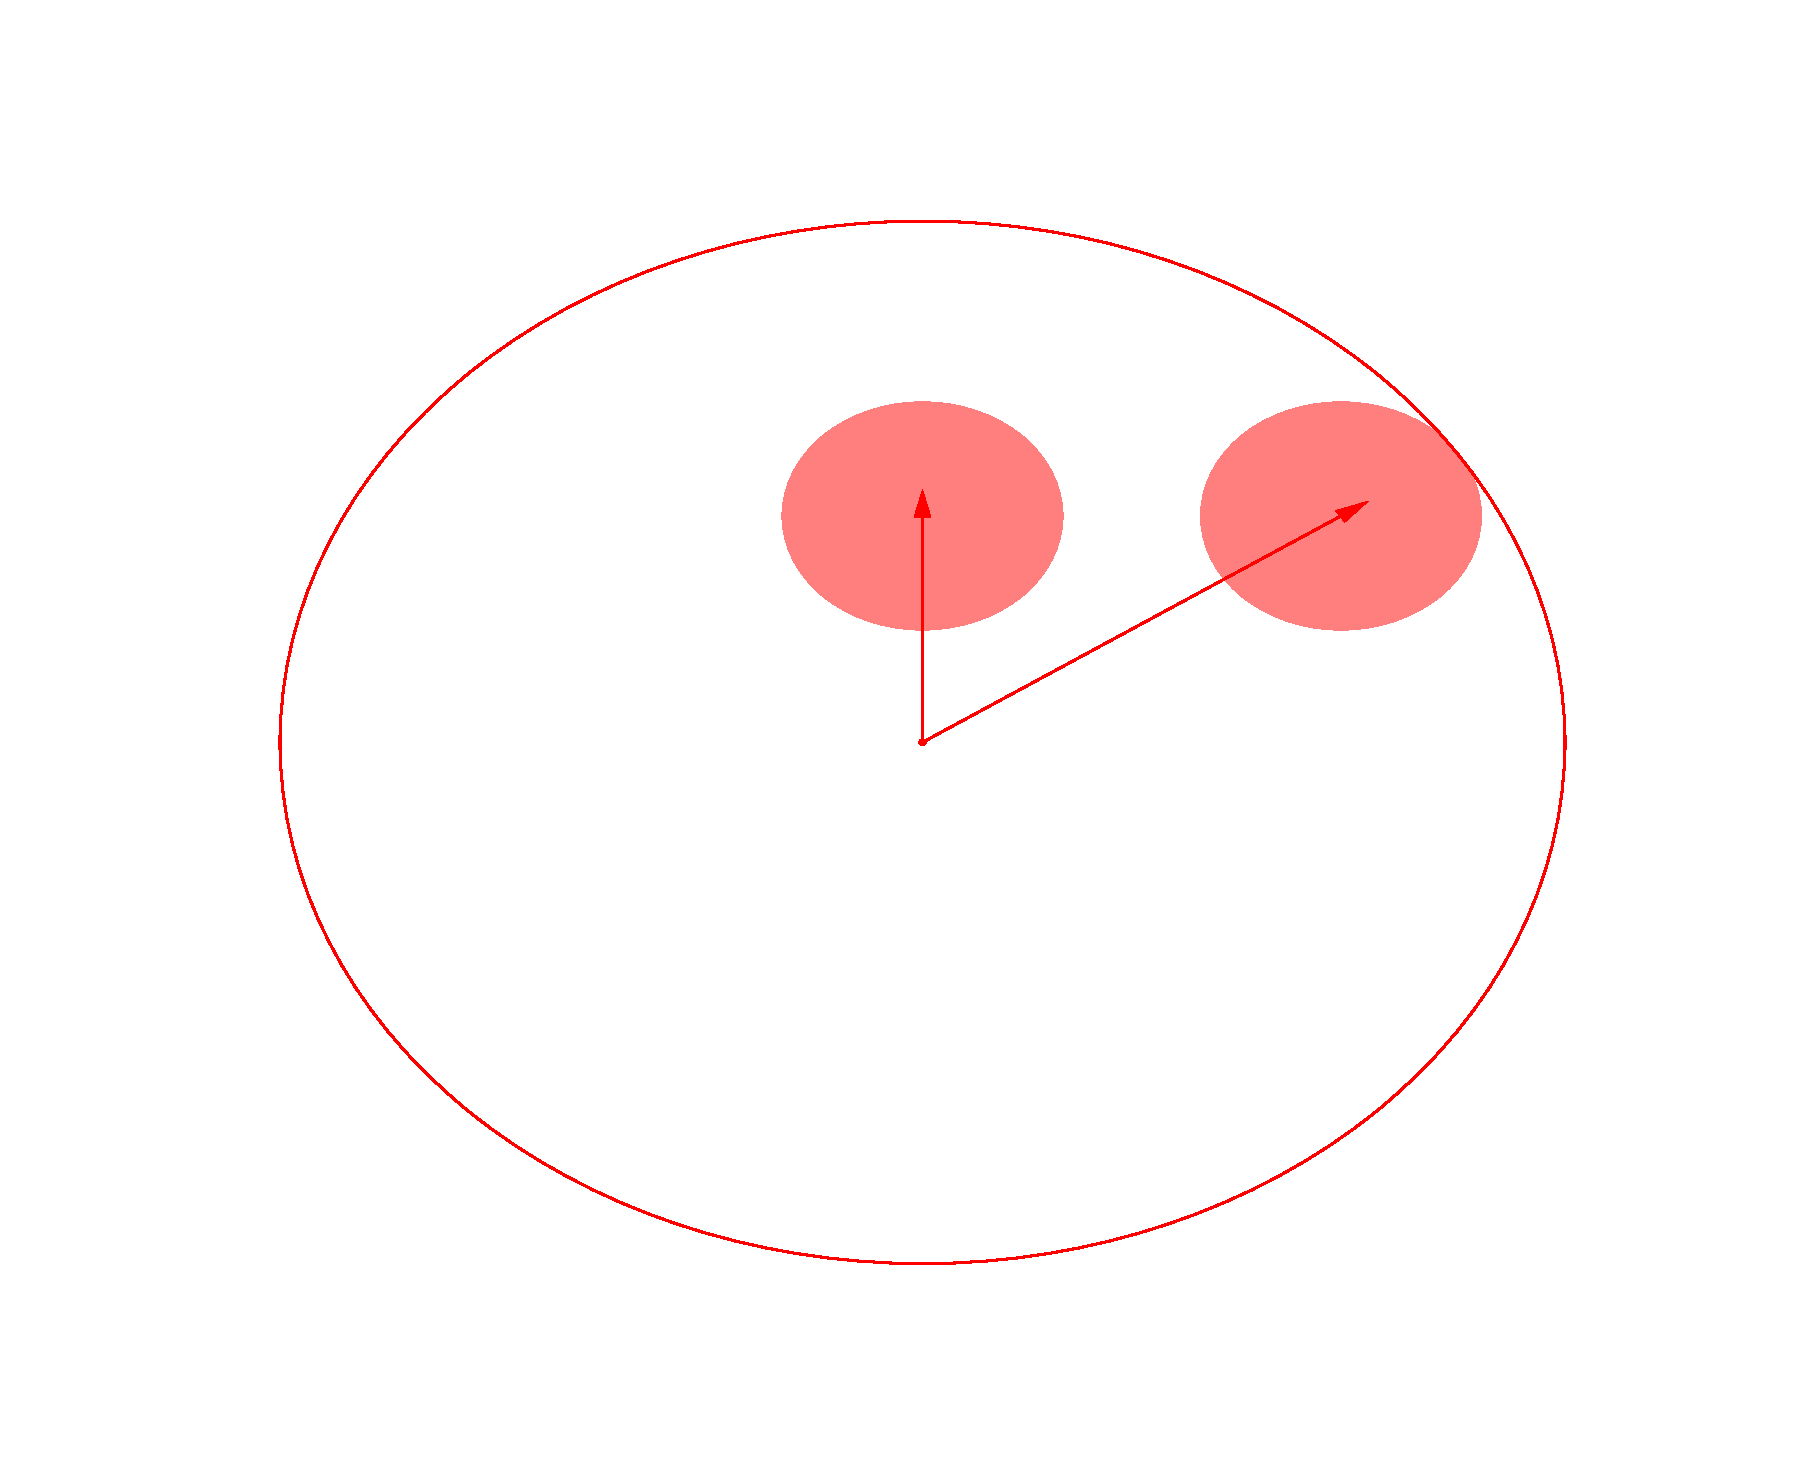
\includegraphics[width=\linewidth,height=\linewidth]{Images/Auxillaries/unoptimised_fig.pdf}
    \caption{unoptimised shape}
  \end{subfigure}
  \begin{subfigure}[b]{0.4\linewidth}
    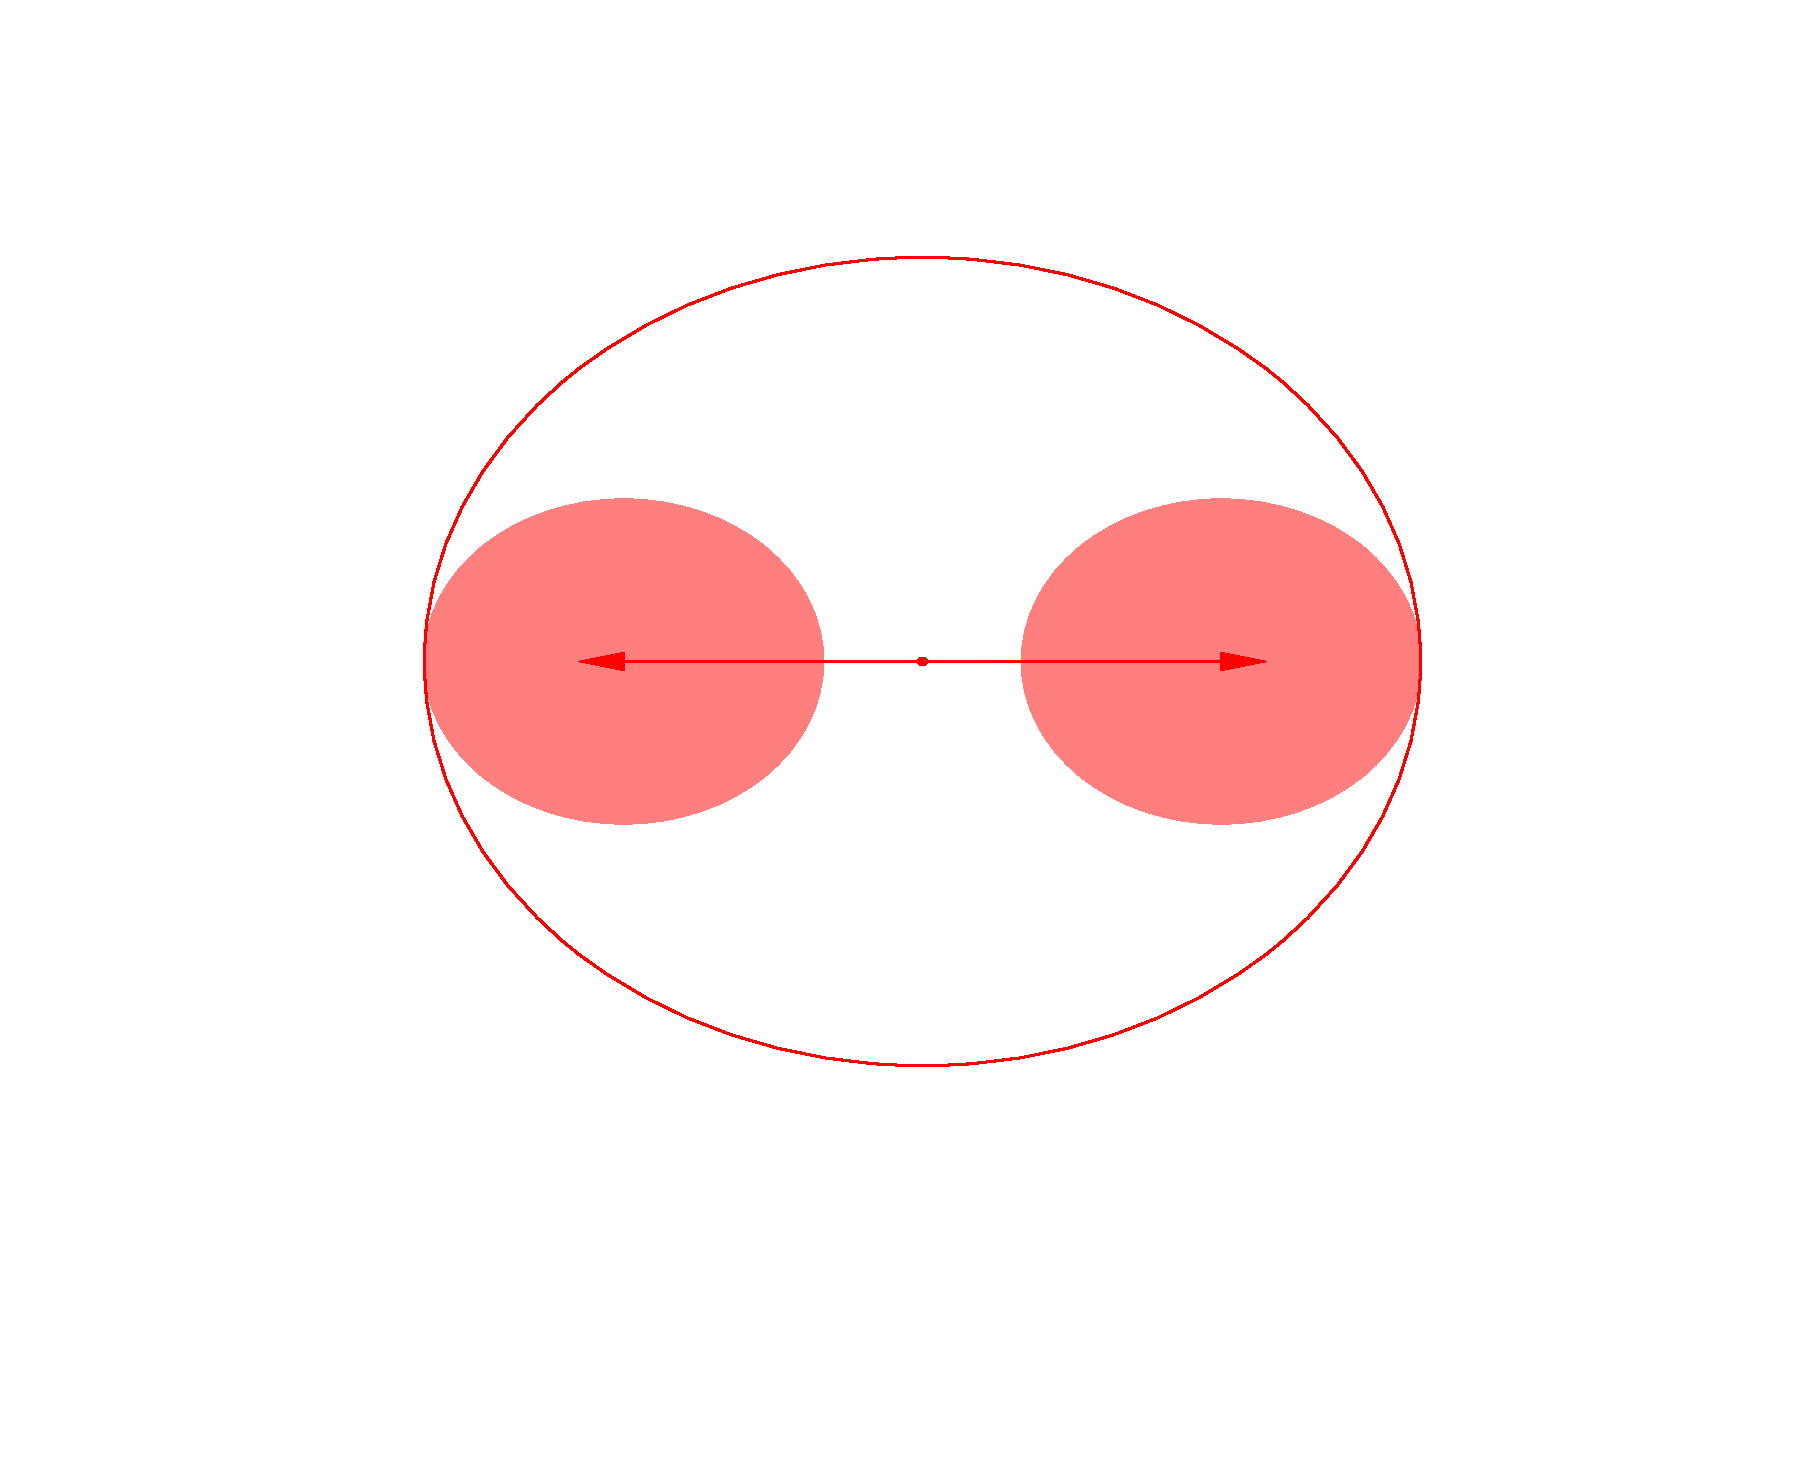
\includegraphics[width=\linewidth,height=\linewidth]{Images/Auxillaries/optimised_fig.pdf}
    \caption{optimised shape}
  \end{subfigure}


\caption{Both shapes are of the same size, but the shape on the left has a greater bounding circle. Using the center of the minimal bounding circle as the origin point enables more effective use of the algorithm. The shape collision is determined only when the bounding circles overlap, and the minimal adjacency matrix cell size depends on their size.}
\end{figure}

\subsection{Other}

The shape area is calculated using the Shapely python geometry library \cite{shapely}. \newline
The images depicting the RSA iterations were created using the Matplotlib python plotting library \cite{matplotlib}.

\subsection{Result Management}

In order to perform analisys of statistical data, some data concerning the algorithm run, besides the output list of shape positions, can be saved. They are saved to the "results.json" file, and include:
\begin{itemize}
  \item Number of shapes and voxels
 	\item Proportion of the world's area covered by the shapes
	\item Time taken to perform each part (A-D) of the algorithm
\end{itemize}
These data are saved per every iteration, as well as a summary, with the total execution time. \newline
Several additional minor result management solutions were temporairly used to create data for the performance examination.


%ACTUAL THESIS: RESULTS INVESTIGATION ====================================================

\chapter{Result Examination}
\section{Performance Evaluation}

As the overall goal of this thesis is to create an efficient implementation of the RSA algorithm, determining the optimal parameters for the shortest execution time is crucial.

\subsection{Theoretical Complexity}

The calculational complexity of the single iteration can be described as: \newline
\begin{equation*}
	O(\text{iteration}) = O(A)+O(B)+O(C)+O(D)+O(E)
\end{equation*}
Where $O(A)$,$O(B)$,$O(C)$ represent the calculational complexities of the parts of the algorithm demonstrated at figure \ref{GPURSABlockDiagramPdf}. The complexity of the figure generation phase is:
\begin{equation*}
	O(A) = O(\text{added shape number}/ \text{number of CUDA threads})
\end{equation*}
Assuming the 'ideal' situation, in which the number of CUDA threads available is greater than the number of added shapes, the complexity is $O(1)$ \newline
The complexity of rejecting new shapes against old ones is: \newline
\begin{gather*}
	O(B) = O(\text{added shape number}/ \text{number of CUDA threads } \cdot \\ \text{ maximum number of shapes in neighborhood})
\end{gather*}
In 'ideal' situation, this will be $O(\text{maximum number of shapes in neighborhood})$ \newline
The complexity of rejecting new shapes against new ones can be described as: \newline
\begin{gather*}
	O(C) = O(\text{number of surviving shapes } \cdot
	\text{ maximum number of shapes in neighborhood} \cdot \\ \text{number of circles in a figure}^2)
\end{gather*}
As this part is not executed in parallel, it's execution time is predicted to be the greatest. Every surviving new shape must be checked against those new other ones, that belong in the same neighborhood. \newline
Voxel splitting is described as: \newline
\begin{equation*}
	O(D) = O(\text{voxel number}/ \text{number of CUDA threads } \cdot 8)
\end{equation*}
Again, in 'ideal' conditions, this value will approach $O(8)$ \newline
Finally, the voxel rejection complexity can be represented as:
\begin{gather*}
	O(B) = O(\text{voxel number } \cdot  \text{ maximum number of shapes in neighborhood } \cdot \\ \text{ number of circles in a figure}^2)
\end{gather*}
While in perfect conditions, this will take only a few iterations, if the number of voxels rises above the capabilities of the GPU, this part may be severely slowing down the execution of the algorithm.

\subsection{Investigating Performance}

Outside of theoretical inquiries, the actual perforance was investigated. All calculations were performed using the 8GB RAM / Intel® Core i5-8250U CPU @ 1.60GHz x 8 / Nvidia® GeForce MX150 / Ubuntu 18.04 laptop. The GPU had 384 CUDA cores operating at a 1708Mhz clock and 2048 MB of memory. \newline
The shape chosen for the preliminary calculations was a dimer, a polydisk made of two intersecting circles of identical radiuses, where the center of one of them is located at a radius distance from another's center. Also, as the overuse of GPU memory has been commonly causing crashes, a limit was imposed on the number of voxels. If the number of voxels reaches more than 1 million, they will not be split any further. While it theoretically warps the results, it is partially an equivalent to setting a high voxel split treshold, and it enables to perform otherwise impossible calculations.

\begin{figure}[H]
  \centering
	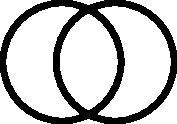
\includegraphics[width=0.3\textwidth,keepaspectratio]{Images/SummaryOptimisation/dimer.pdf}
	\caption{The dimer used in the calculations.}
	\label{summary_dimer}
\end{figure}
The RSA algorithm was performed using this shape, for a set of configurations. These included space sizes ($25 \times 25$, $50 \times 50$, $75 \times 75$, $100 \times 100$ cells), different numbers of polydisks added (512, $512 \cdot 2$, $512 \cdot 4$, $512 \cdot 8$, $512 \cdot 16$) and different voxel split tresholds (0.1,0.3,0.5,0.7,0.9). The cell size is equal to the polydisk's minimal bounding circle radius.
If the proportion of shapes, that were not succesfully inserted, is above the voxel split treshold, then they are split. The added shape number comes in multiplies of 512 in order to effectively utilise the 512 threads in CUDA block.

\begin{figure}[H]

\begin{subfigure}[b]{\linewidth}
  \centering
	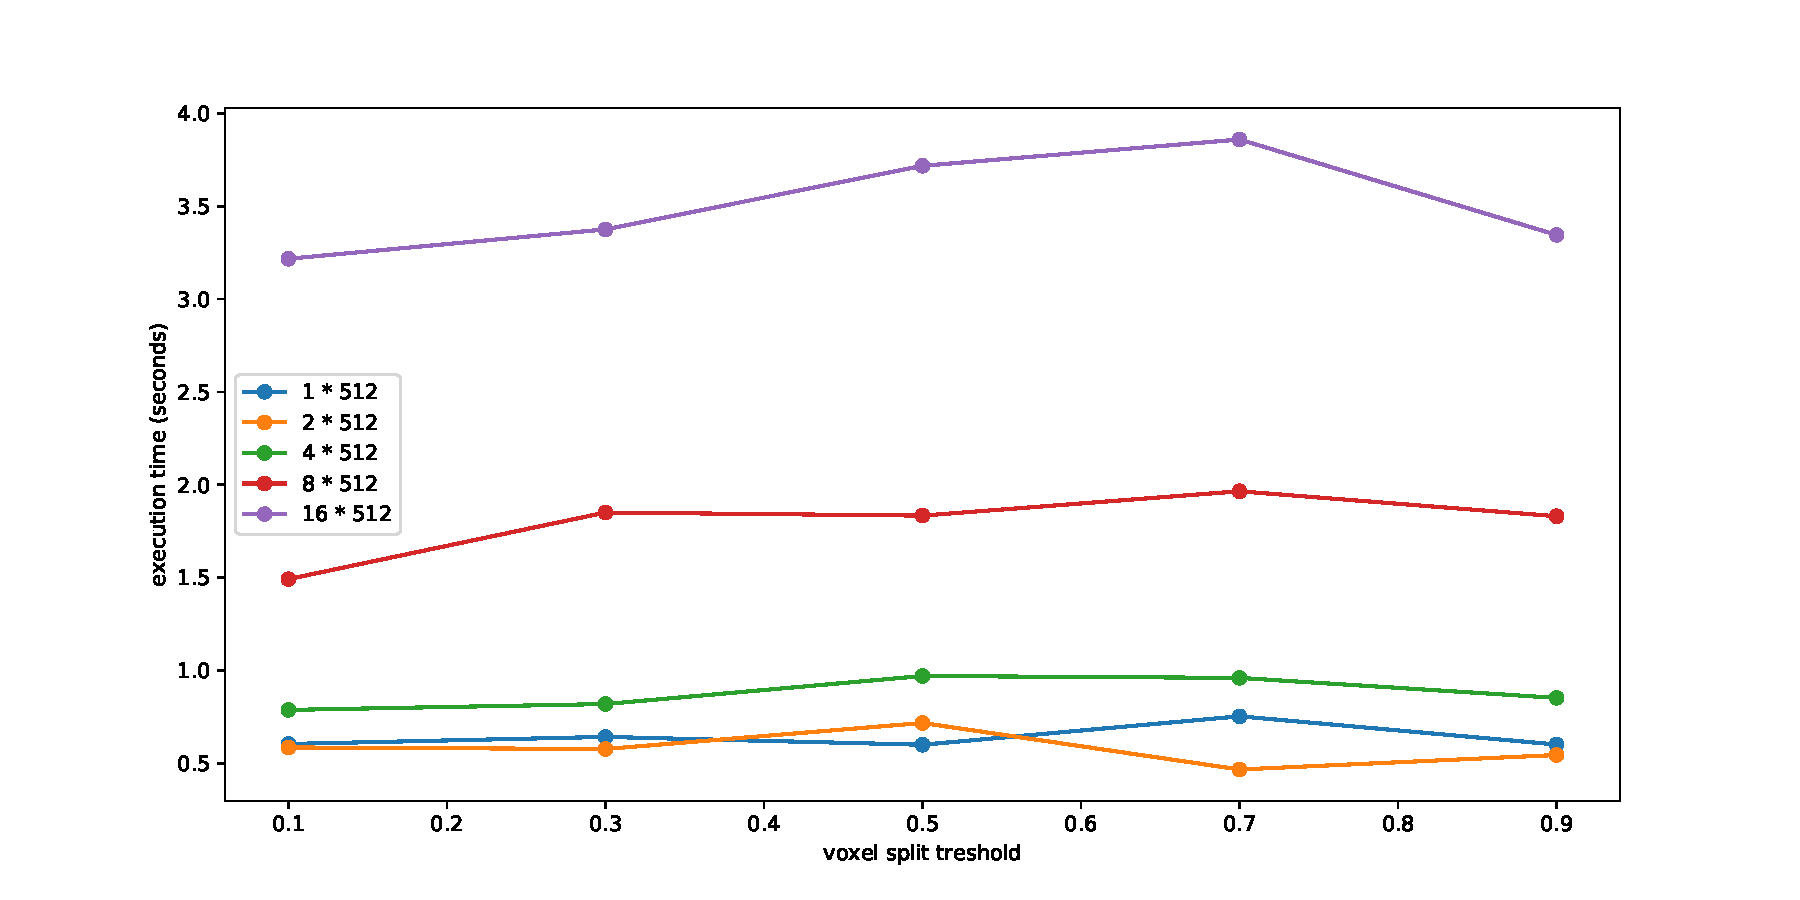
\includegraphics[width=\linewidth,keepaspectratio]{Images/SummaryOptimisation/results_25.pdf}
	\caption{Space size: $25 \times 25$ cells. Execution time (seconds) for different voxel split tresholds. Different plots represent different added shape numbers. The results are an average per 5 trials at each different configuration.}
	\label{summary_res25}
\end{subfigure}

\end{figure}
\begin{figure}[H]\ContinuedFloat

\begin{subfigure}[b]{\linewidth}
  \centering
	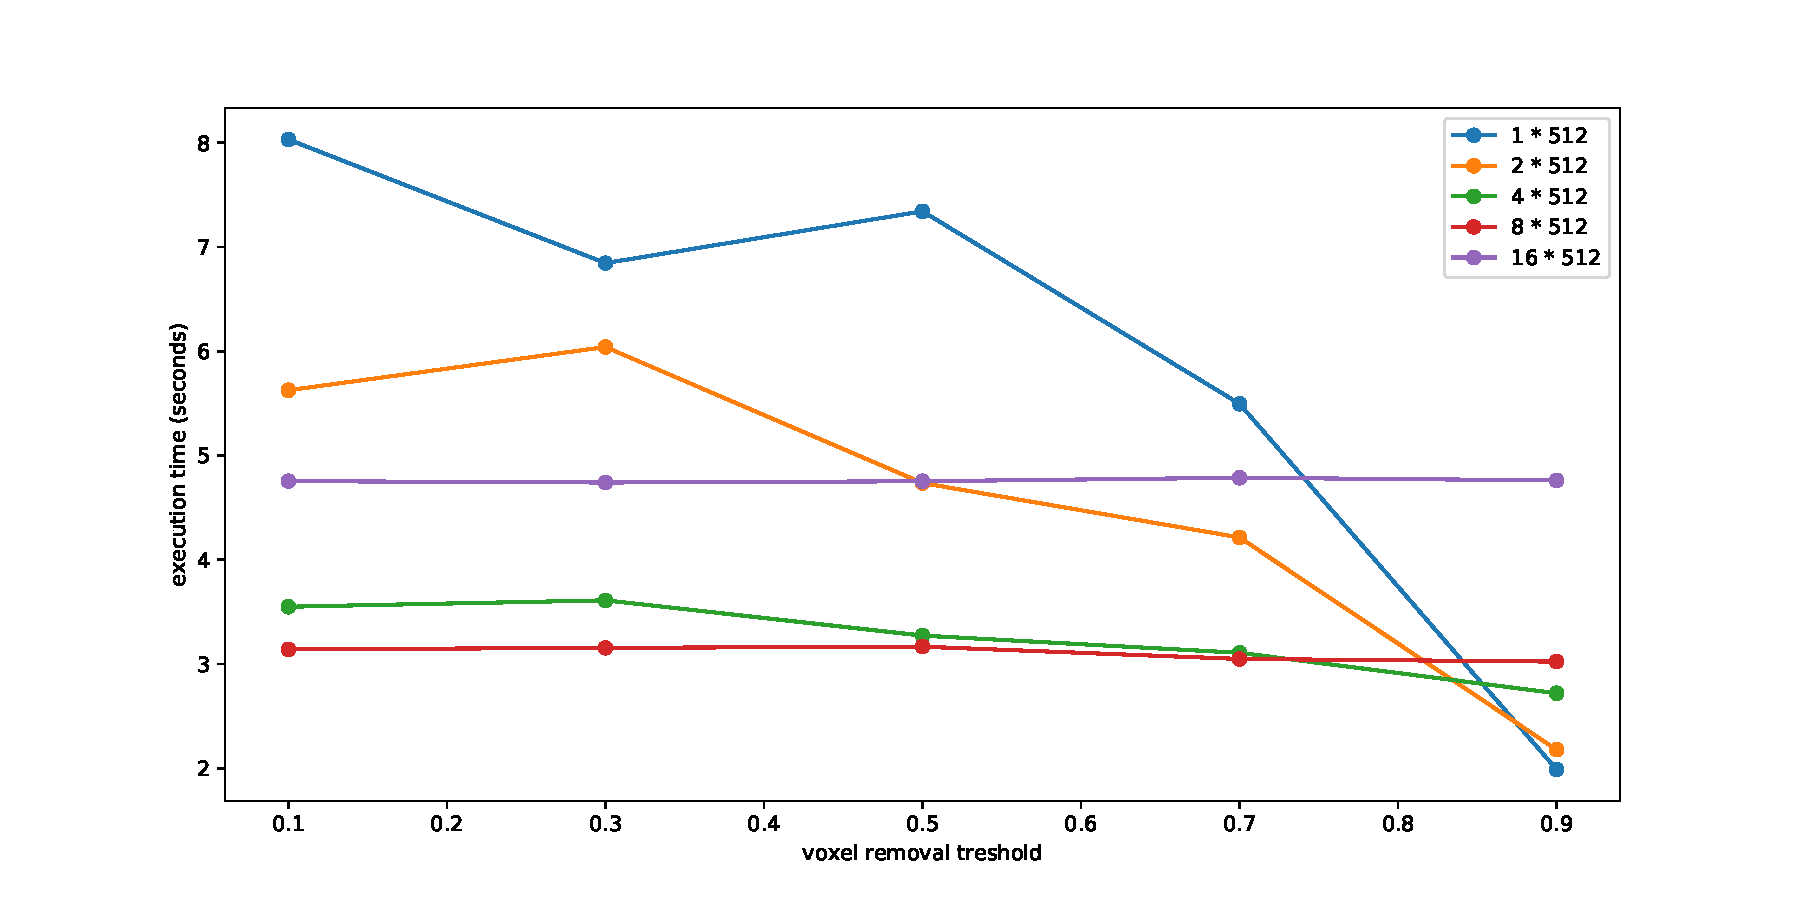
\includegraphics[width=\linewidth,keepaspectratio]{Images/SummaryOptimisation/results_50.pdf}
	\caption{Space size: $50 \times 50$ cells.}
	\label{summary_res50}
\end{subfigure}

\end{figure}
\begin{figure}[H]\ContinuedFloat

\begin{subfigure}[b]{\linewidth}
  \centering
	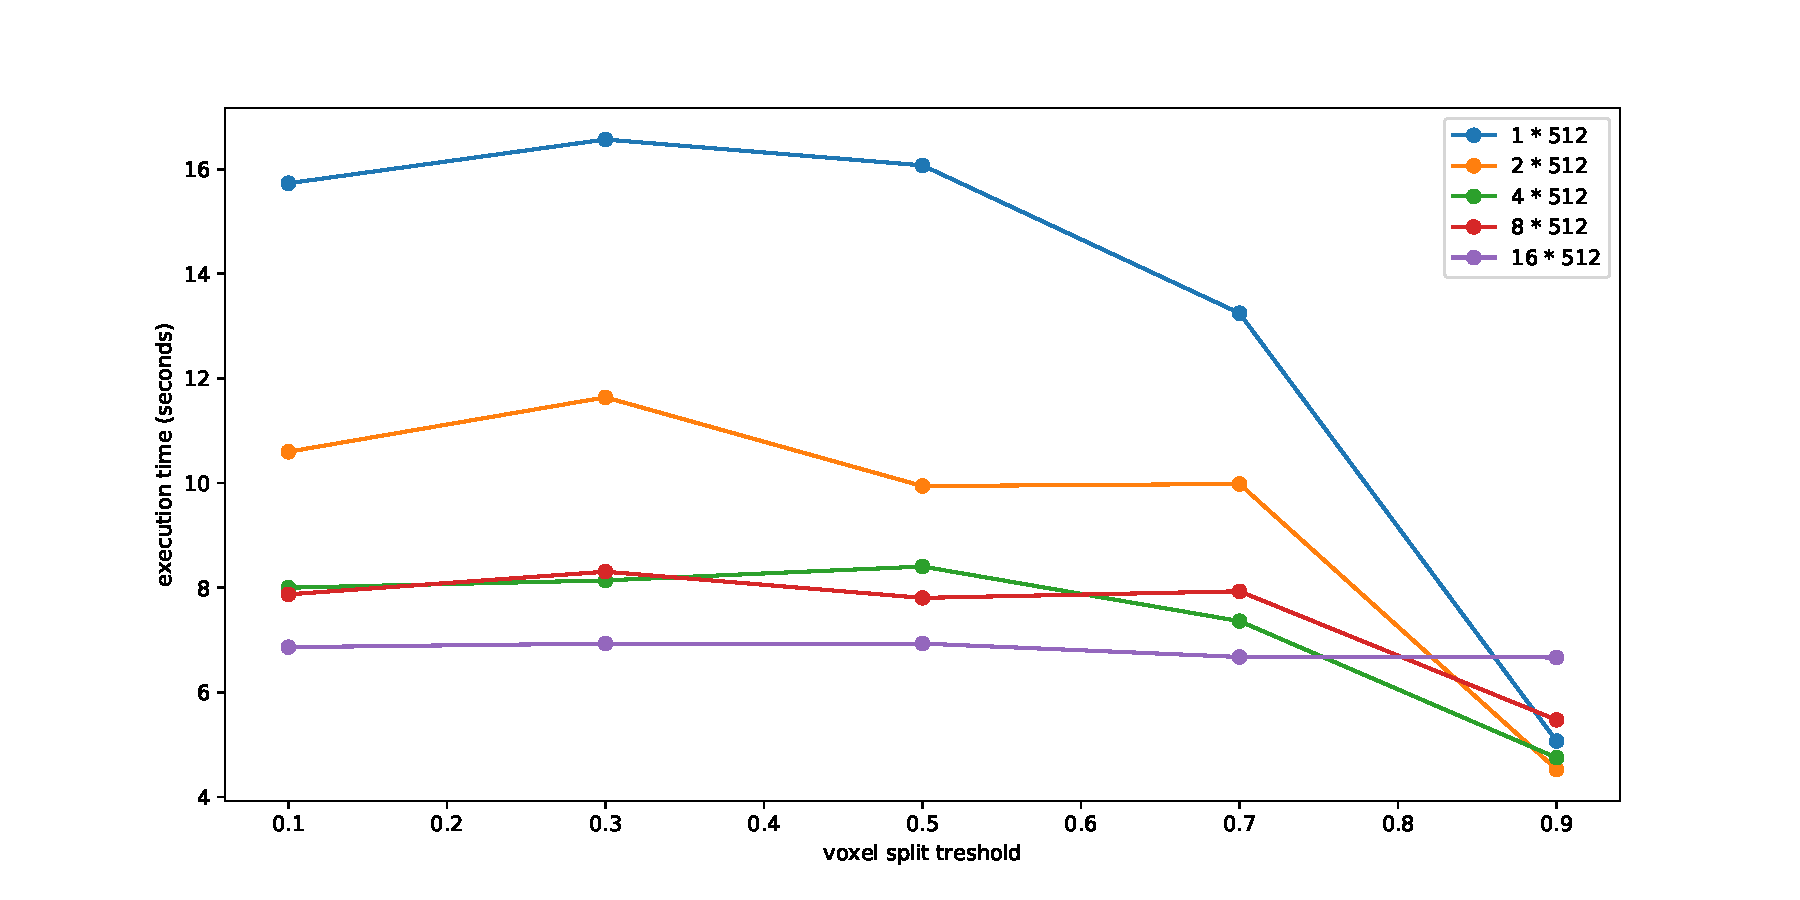
\includegraphics[width=\linewidth,keepaspectratio]{Images/SummaryOptimisation/results_75.pdf}
	\caption{Space size: $75 \times 75$ cells. }
	\label{summary_res75}
\end{subfigure}

\end{figure}
\begin{figure}[H]\ContinuedFloat

\begin{subfigure}[b]{\linewidth}
  \centering
	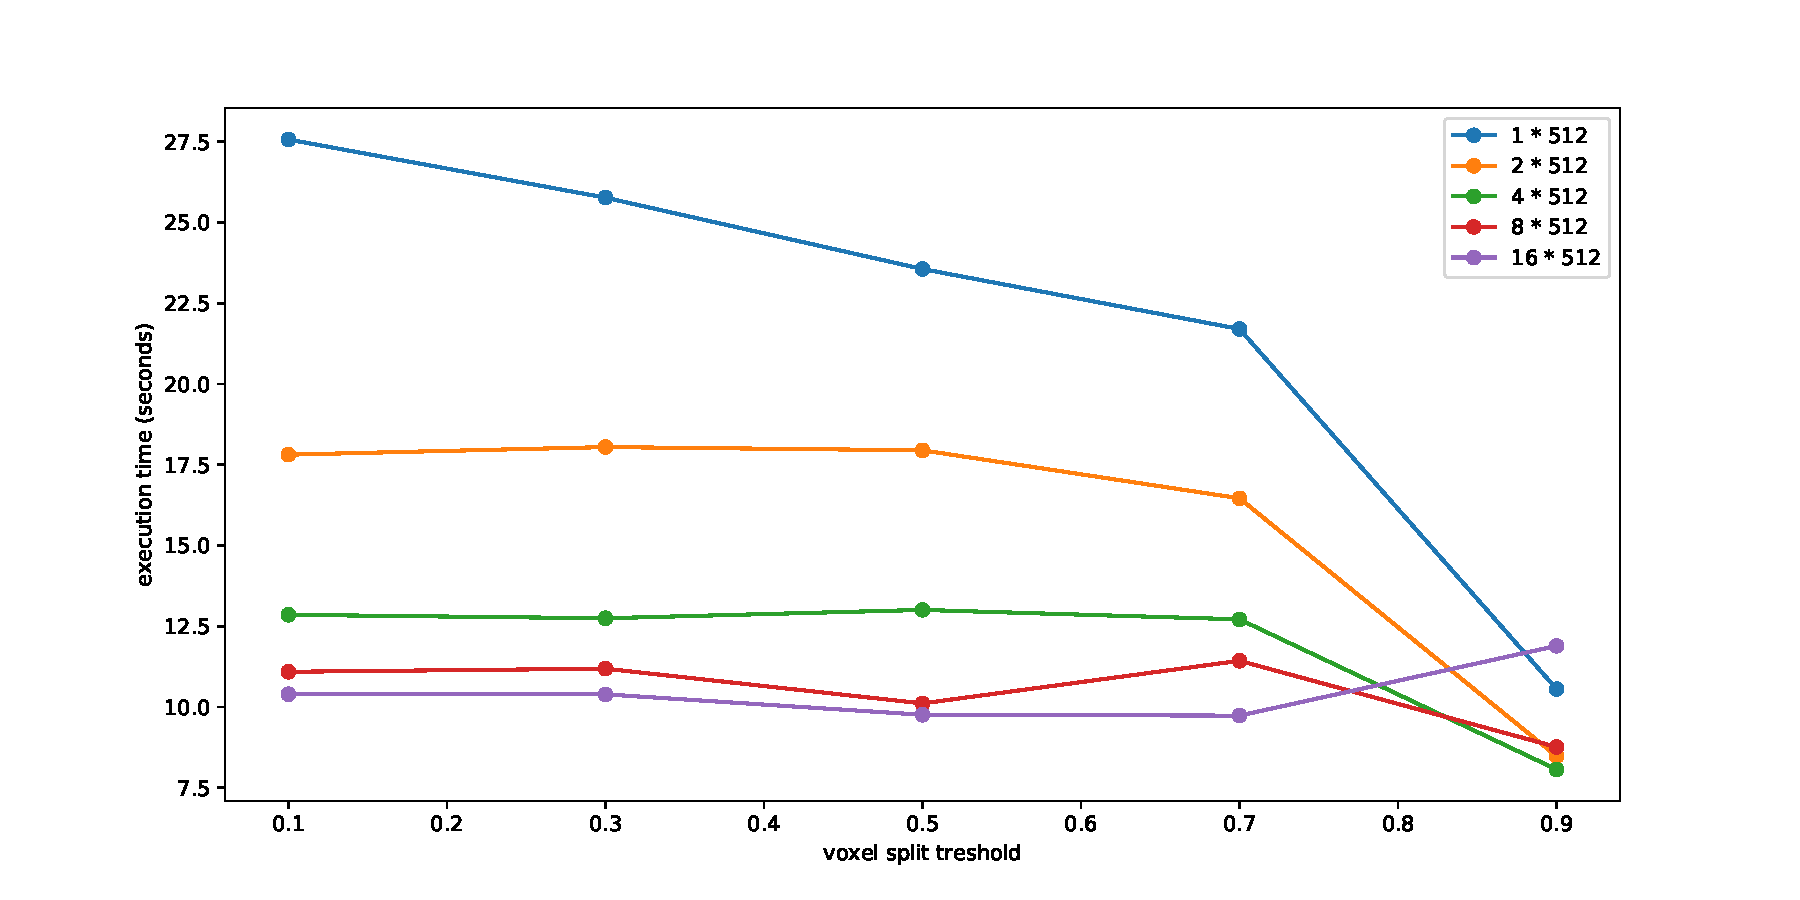
\includegraphics[width=\linewidth,keepaspectratio]{Images/SummaryOptimisation/results_100.pdf}
	\caption{Space size: $100 \times 100$ cells.}
	\label{summary_res100}
\end{subfigure}

\caption{Comparison of execution times of the proposed algorithm, given different execution parameters.}

\end{figure}

The relationship that is relatively easy to discern, is that the optimal number of shapes added is related to the space size. At $25 \times 25$ cells, the most optimal added cell number is 512, however for $100 \times 100$, it's $512 \cdot 16$. While these results are consistent for most voxel split tresholds, at around 0.9, most execution times are both the lowest, and fairly similar across different added shape numbers. In order to investigate how exactly do these results appear, a more detailed look was taken at the process:

\begin{figure}[H]
  \centering
	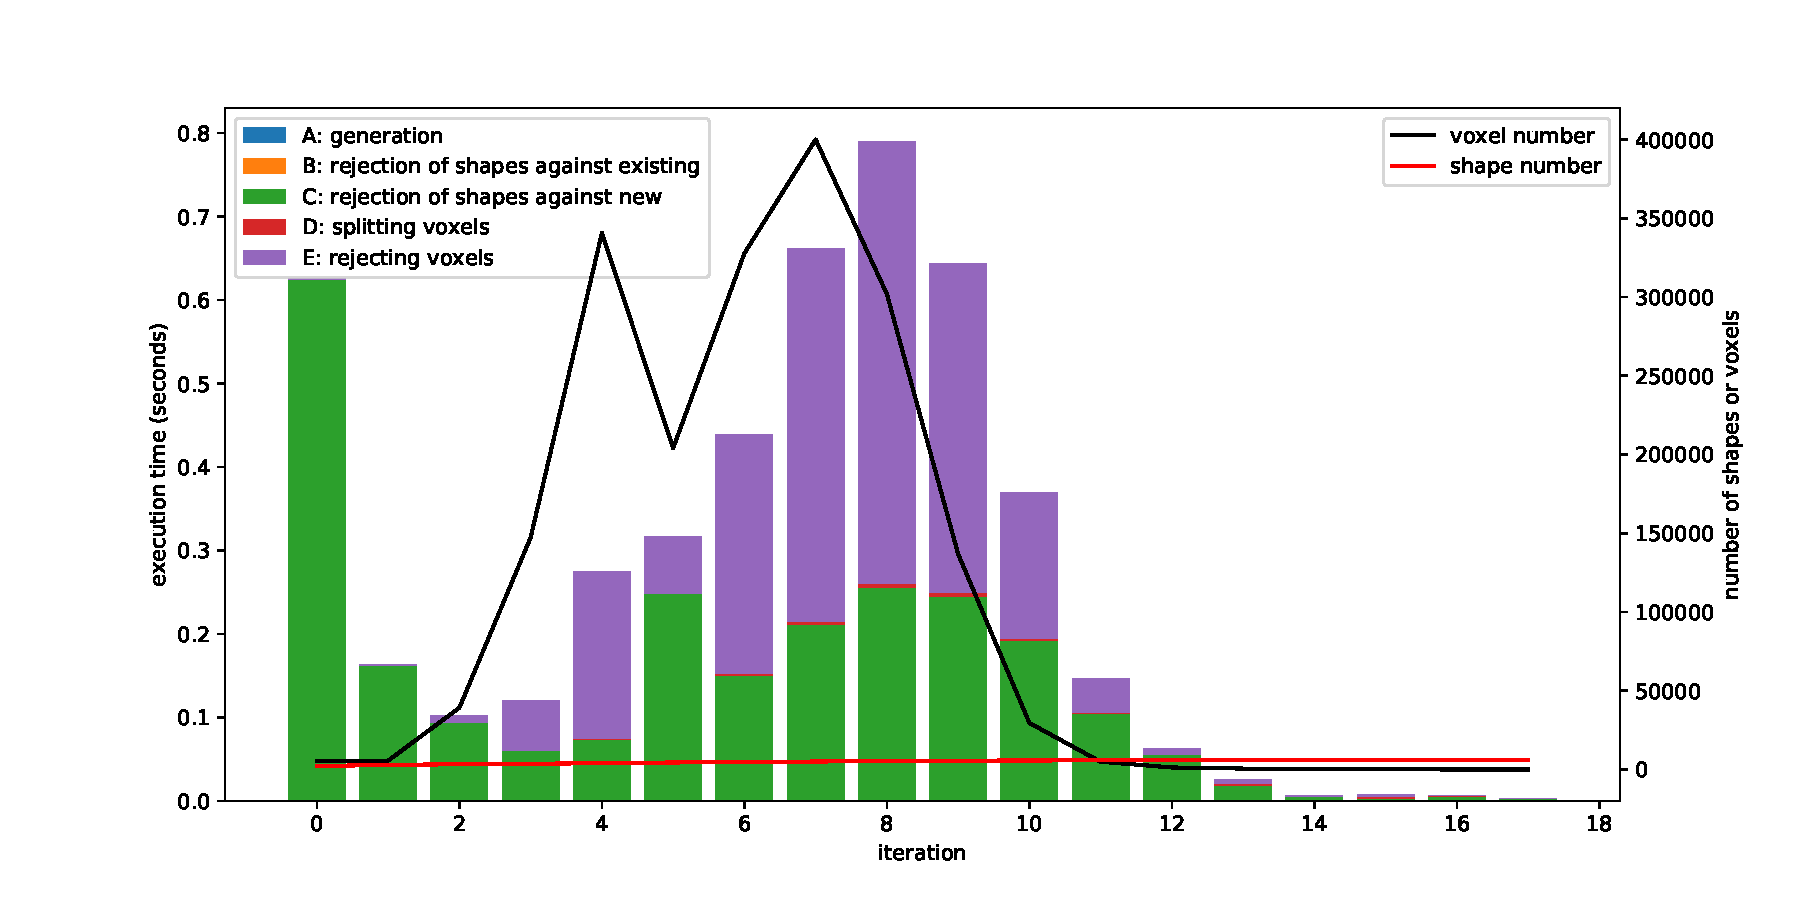
\includegraphics[width=0.9\textwidth,keepaspectratio]{Images/SummaryOptimisation/iter_75_512x8_09.pdf}
	\caption{More detailed look into a single execution of the algorithm at space of $75 \times 75$ cells. Added shape number is $512 \cdot 8$, voxel removal treshold at 0.9. The bar chart represents the time spent by algorithm at a particular execution part, at iteration. The line chart represents the numbers of voxels and shapes at given iterations.}
	\label{summary_detail_75_512x8_09}
\end{figure}

At one of the optimal configurations for $75 \times 75$ cell sized space, the total execution time was 4.772 seconds. Of which, 2.509 was devoted to rejecting shapes against other new shapes, making it 52.6\% of the total time. As the number of voxels skyrocketed at around third and seventh iterations, the time devoted to rejecting voxels also went up.

\begin{figure}[H]
  \centering
	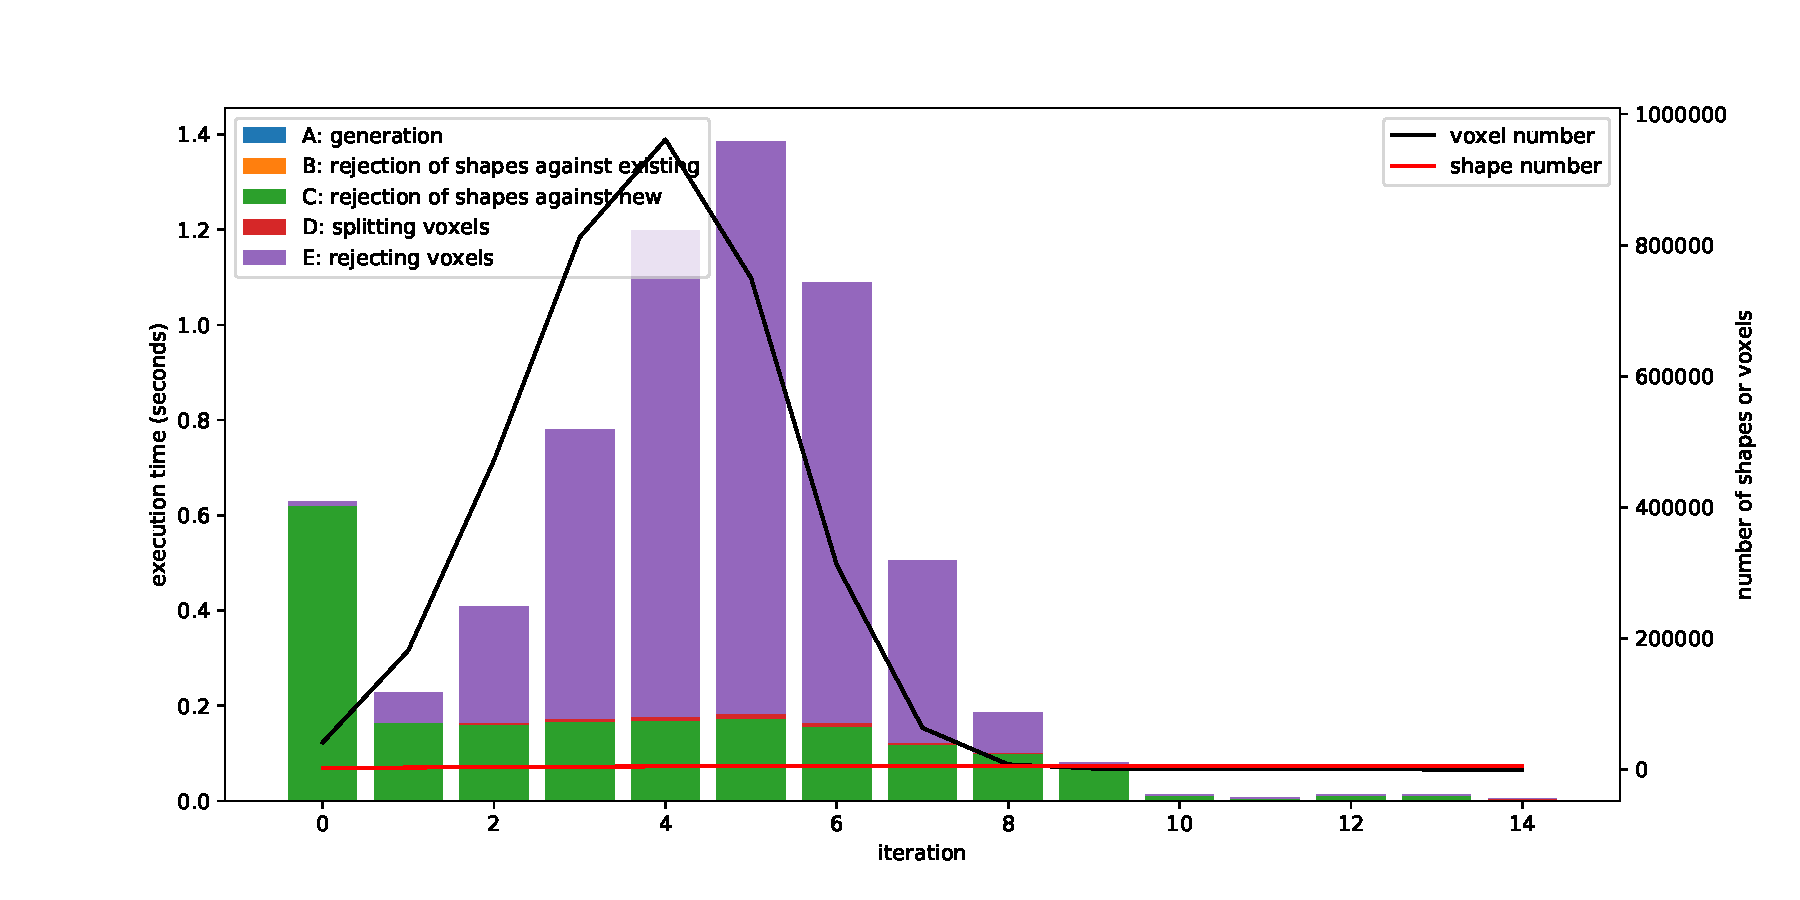
\includegraphics[width=0.9\textwidth,keepaspectratio]{Images/SummaryOptimisation/iter_75_512x8_03.pdf}
	\caption{More detailed look into a single execution of the algorithm at space of $75 \times 75$ cells. Added shape number is $512 \cdot 8$, voxel removal treshold at 0.3.}
	\label{summary_detail_75_512x8_03}
\end{figure}

At the less optimal configuration, where the voxel removal treshold was changed to 0.3, the total time required for rejection of shapes against new fell; It was 1.943 seconds, 29.9\% of the total of 6.548 seconds. However the total time grew, as the 4.553 seconds of voxel rejection slowed down the algorithm.

\begin{figure}[H]
  \centering
	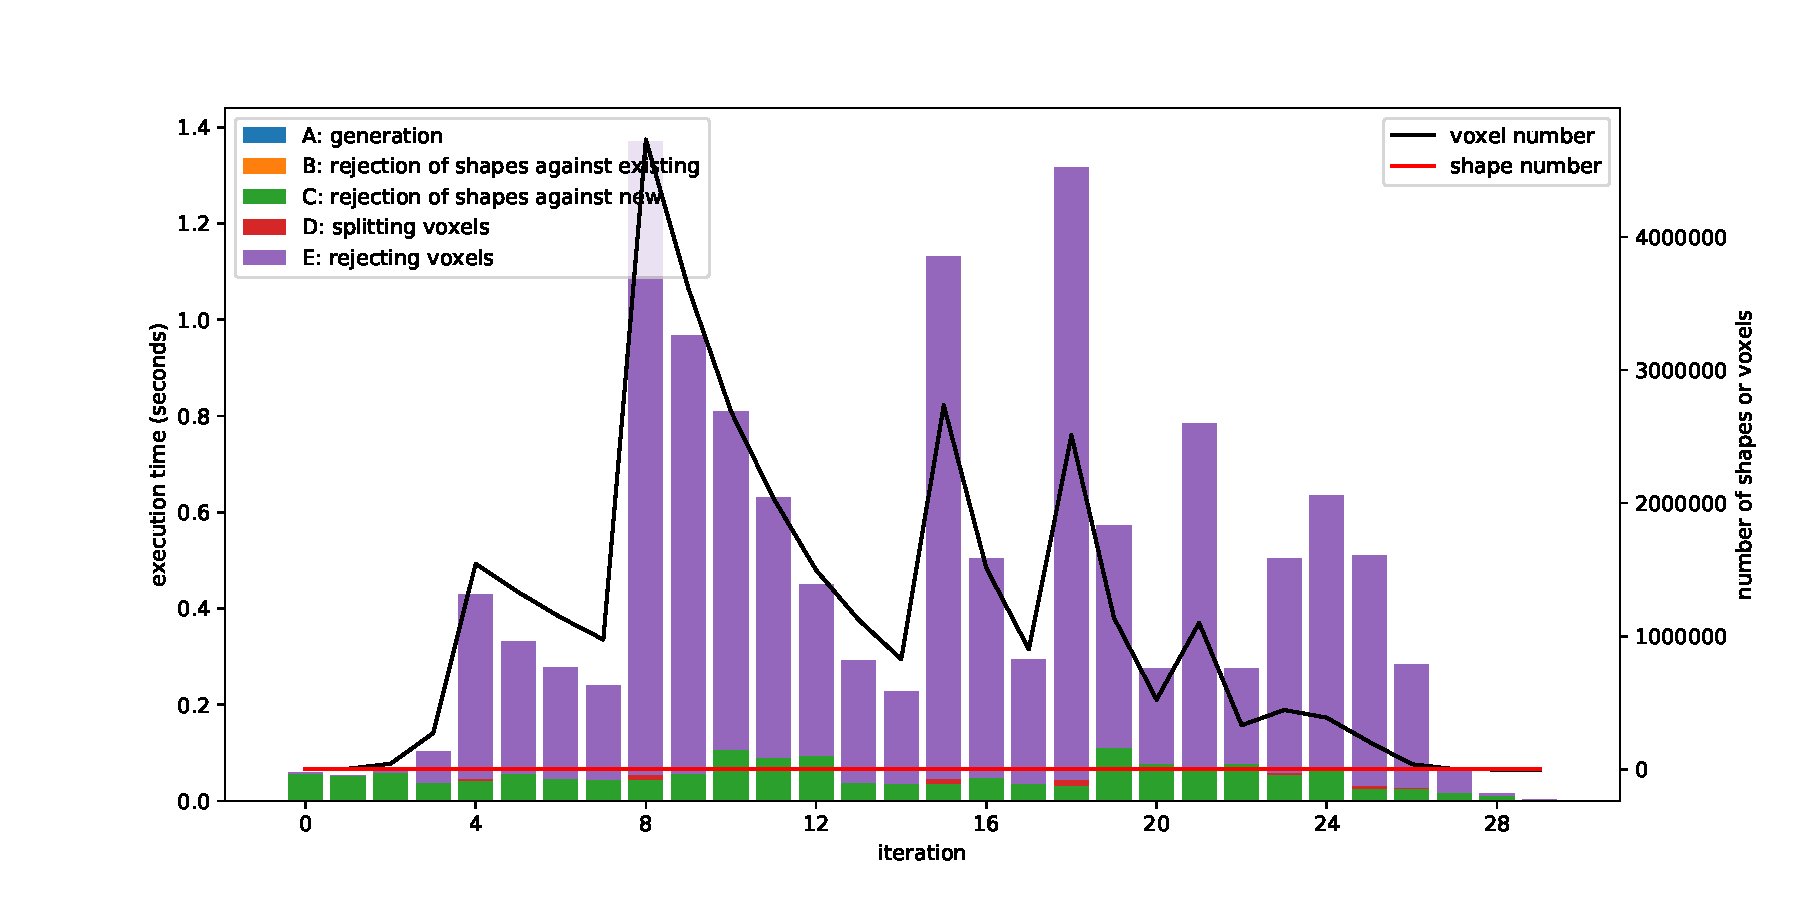
\includegraphics[width=0.9\textwidth,keepaspectratio]{Images/SummaryOptimisation/iter_75_512x1_03.pdf}
	\caption{More detailed look into a single execution of the algorithm at space of $75 \times 75$ cells. Added shape number is 512*1, voxel removal treshold at 0.3.}
	\label{summary_detail_75_512x1_03}
\end{figure}

At the configuration involving only 512 added shapes and voxel split treshold at 0.3, the time spent at rejection of shapes against new ones fell again. It was at 1.551 seconds, while the voxel rejection time grew to 11.865 seconds, with total of 13.487. \newline

In summary, the execution time optimisation is a race between making the time taken by voxel rejection, and shape rejection against new shapes. The first one grows when the voxels are rejected early, as demonstrated on \ref{summary_detail_75_512x8_03}. If the number of added shapes is small, the number of iteration grows, as it takes more time to fill the packing and reject the voxels, by adding shapes in their place. Utilising a GPU with greater capabilities, both memory and processing-power wise may cut the time on the voxel rejection. \newline
In this implementation, the voxels are primarily a mean to check if any new shapes can be added, rather than an acceleration tool for adding them. A possible improvement for the entire process would be to dynamically change the added shape number, depending on the already covered area or voxel number, as the current solution involves static value.

\begin{figure}[H]
  \centering
	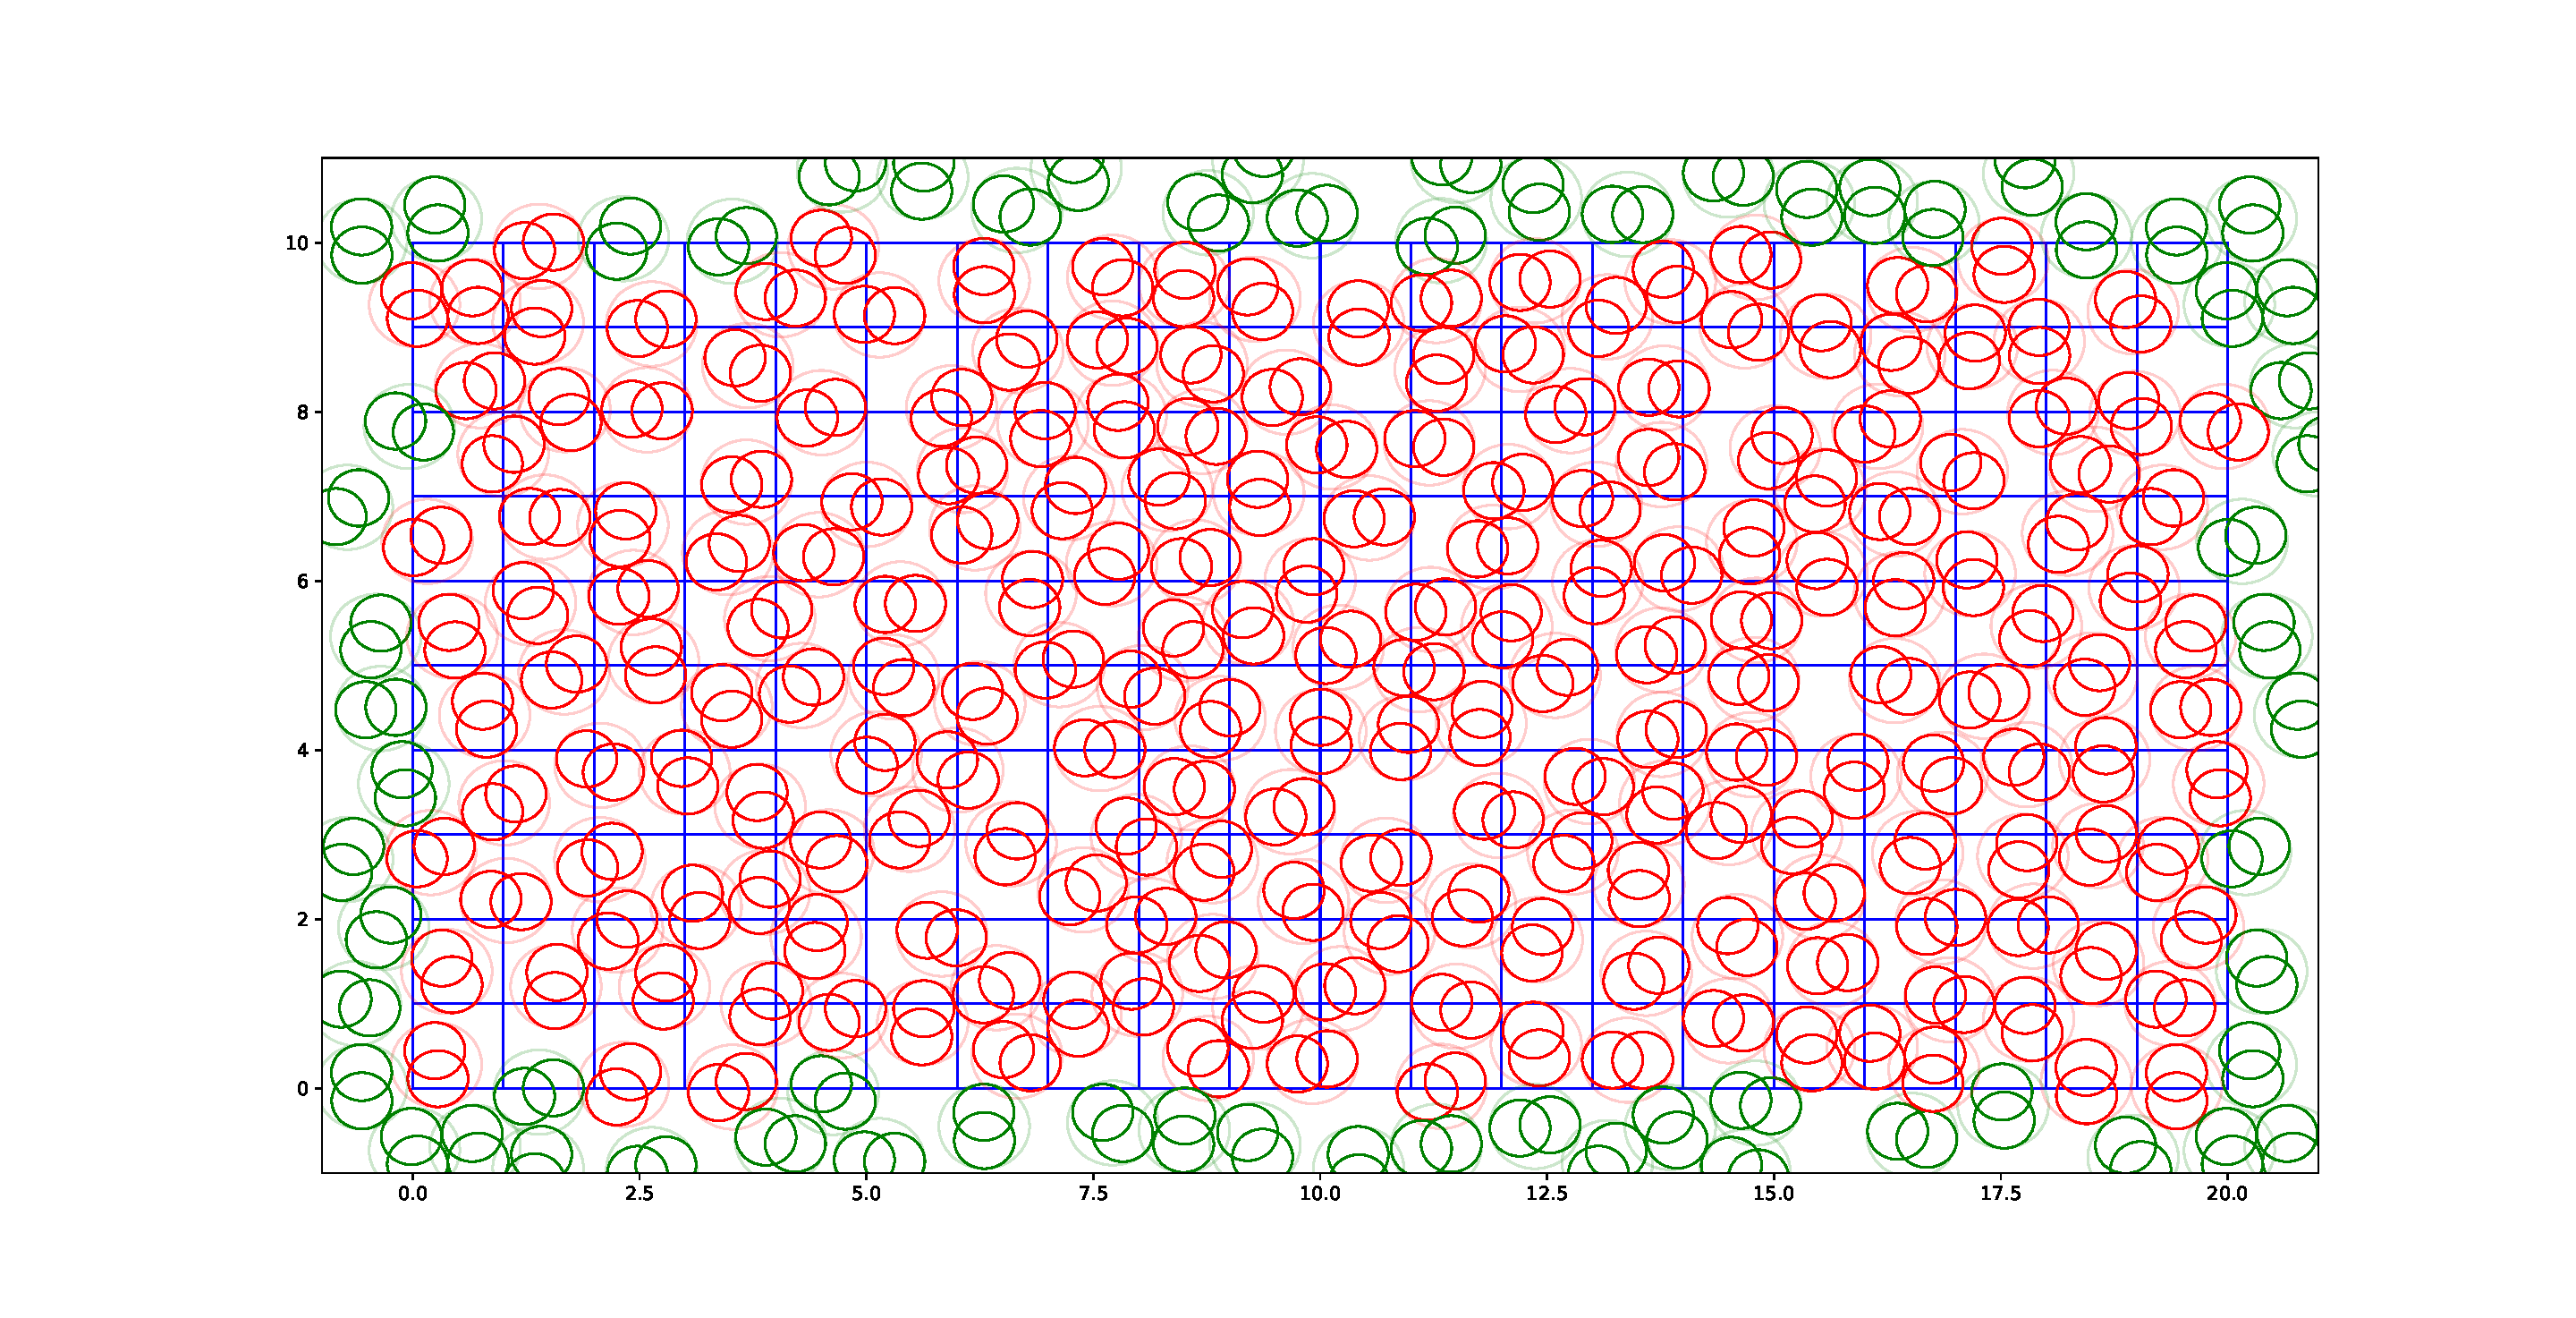
\includegraphics[width=0.9\textwidth,keepaspectratio]{Images/SummaryOptimisation/dimer_ready.pdf}
	\caption{The end result of the execution of the algorithm for a space sized at $20 \times 10$ cells, with the dimer used in the calculations}
	\label{summary_dimer_ready}
\end{figure}

\section{Comparison to the CPU Based Algorithm}

The goal of the proposed algorithm is to create a more efficient approach to the RSA algorithm. In order to evaluate this efficiency, it was compared to the pre existing, CPU based algorithm, the 'RSA3D', developed by Michał Cieśla \cite{ciesla}. The GPU algorithm was implemented using C++ programming language and the OpemMP package. It is parallel on the CPU level, utilising multiple threads. The RSA3D utilised up to 8 threads, as this was the CPU limit. \newline


\begin{figure}[H]
  \centering
	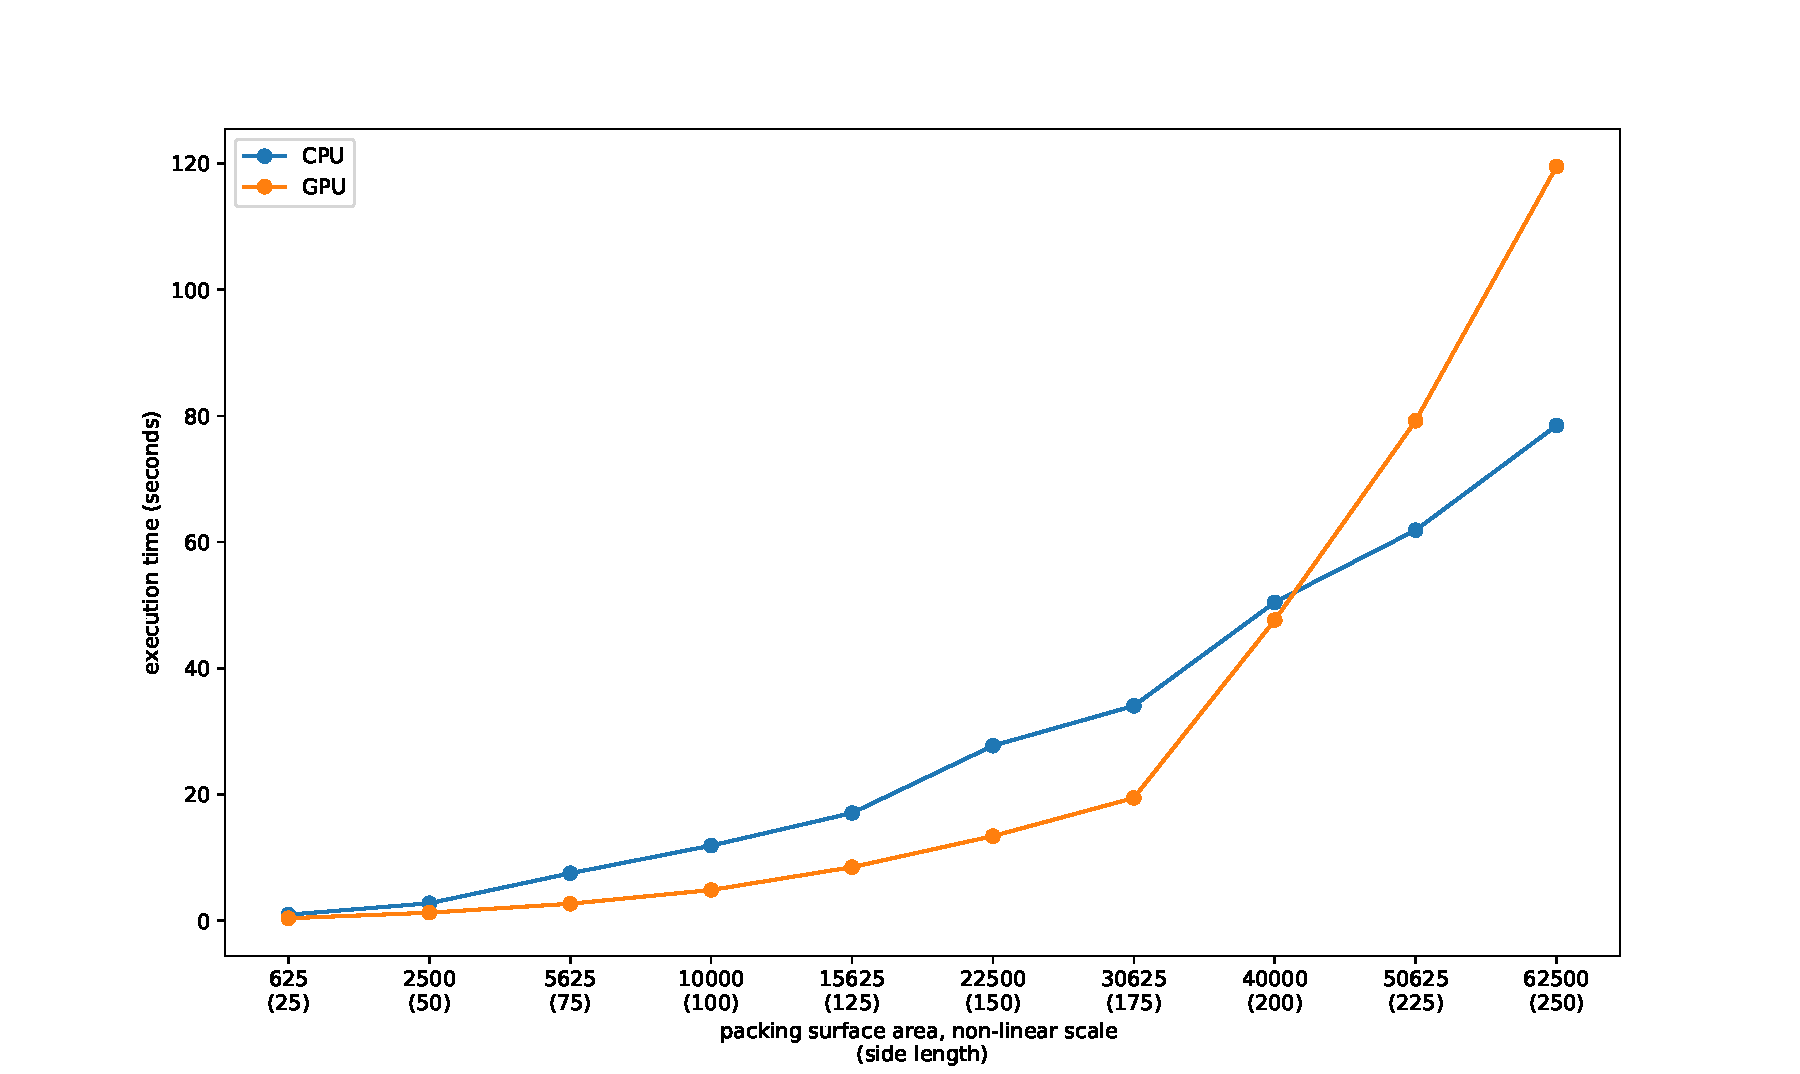
\includegraphics[width=0.9\textwidth,keepaspectratio]{Images/SummaryComparison/basic_comparison.pdf}
	\caption{Comparison between the execution time of CPU based implementation and the proposed algorithm. The algorithms were run over a set of square packing spaces with increasing sizes, 5 trials at each. The voxel split treshold was equal to 0.98, while the number of inserted figures were a function of packing side size at $f(s) = 512 \cdot 2 \cdot s/25 $ }
	\label{summary_comparison}
\end{figure}

The proposed algorithm performed with a shorter execution time for packings with sizes from $25 \times 25$ to $200 \times 200$ cells. At greater packing sizes, the proposed algorithm's execution time has started growing at an increasing rate, unlike the CPU based approach. \newline
The general expectation is that the GPU will perform operations more efficiently than CPU if it operates on large amount of data at once. However, here this expectation is subverted, as the GPU-based algorithm outpaces the CPU-based on the smaller packings. It is suprising, as also the sequential parts of the algorithm were implemented using Python. The interpreted language is in most cases slower than an equivalent code written in C++. The conclusion is that, its most likely that the parallelisation utilising GPU was the key to outpacing the C++ implementation.\newline
The advantage over the CPU based algorithm ends at the packing size of around $200 \times 200$ cells. It can be attributed to the limitations of the GPU, as the number of split voxels grows. The CPU holds an advantage in the accesible memory size. Also, there is no need to transfer data between the GPU and CPU memory.

\begin{figure}[H]
  \centering
	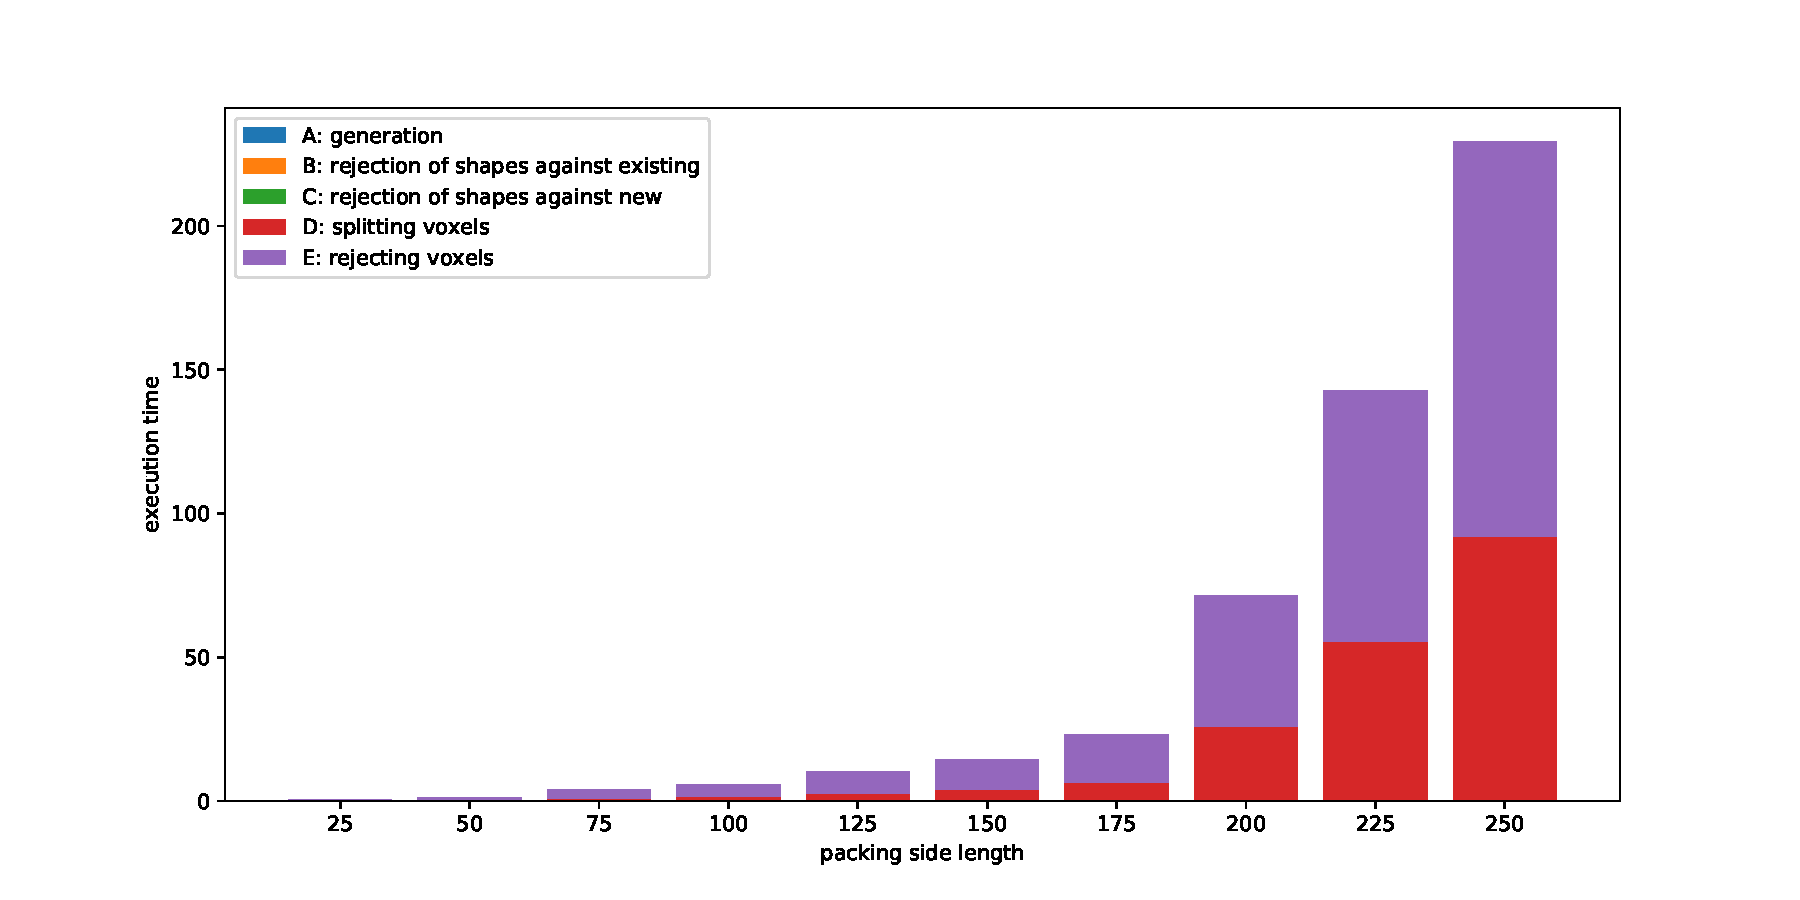
\includegraphics[width=0.9\textwidth,keepaspectratio]{Images/SummaryComparison/parts_total.pdf}
	\caption{Execution time and it's elements for different packing sizes. Each bar contains the total time within the executon that was taken by the given part. The algorithm uses the same configuration as in \ref{summary_comparison}. }
	\label{summary_times_total}
\end{figure}

\begin{figure}[H]
  \centering
	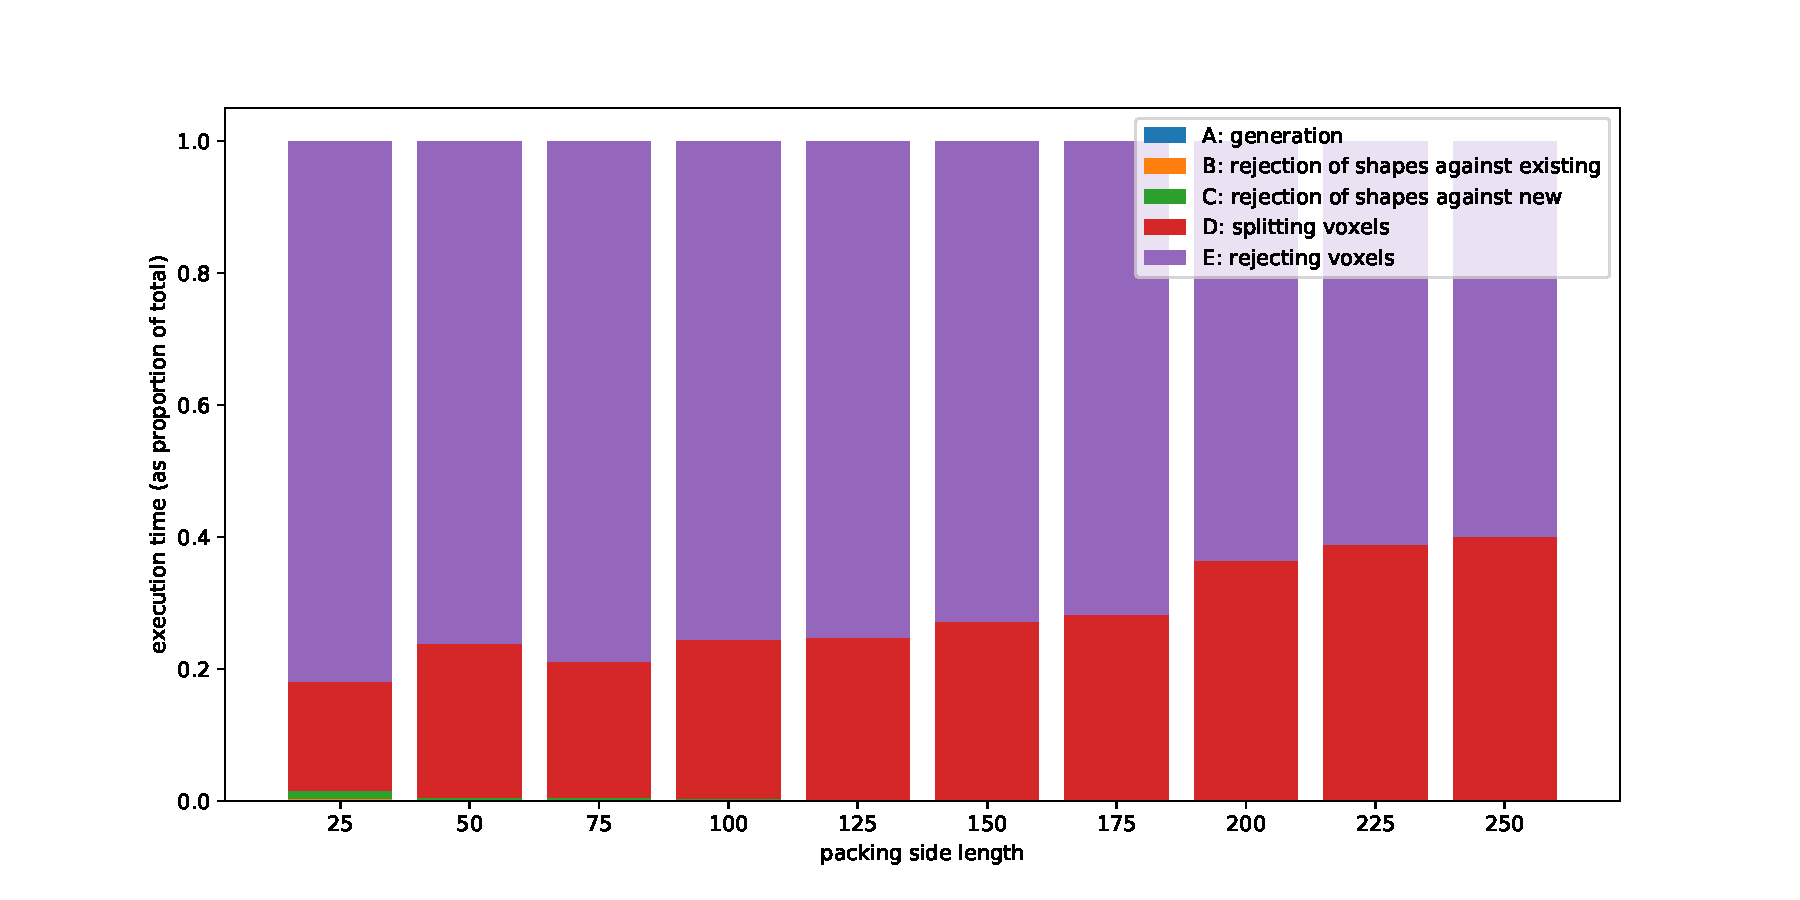
\includegraphics[width=0.9\textwidth,keepaspectratio]{Images/SummaryComparison/parts_proportional.pdf}
	\caption{Execution times of different parts of the algorithm, as in proportion to the total time.}
	\label{summary_times_proportional}
\end{figure}

The majority of the execution time is taken by the voxel management. The time taken by splitting grows steadily in proportion to voxel rejection. This hints at performance problems related to the GPU processing power, memory, and data transfer limitations being the cause.


\section{Summary}

The Random Sequential Adsorption algorithm utilising the GPU has been proposed, implemented and evaluated. It was shown that the execution can be accelerated through parallelization of most of it's parts. The implementation shows potential, especially considering that it's sequential parts have been implemented using a relatively slow interpreted language. It has manged to outperform the previous, CPU-level parallel, solution at a limited range of packing space sizes. \newline
The program has however shown it's limitations. It's execution time is longer than the CPU solution on large packings. Investigaition into the execution of the algorithm with different parameters shows that it is hampered by inefficient voxel management, possibly caused by the GPU limitations. It is possible, that utilising the more powerful GPUs and further optimisations could improve the robustness of the algorithm. It could enable the algorithm to operate efficiently on wider ranges of packing sizes, with greater speed.

%ACTUAL THESIS: BIBLIOGRAPHY ====================================================

\newpage
\printbibliography

\end{document}
